\title{クラウドファンディングにおける成功の判別分析}
\author{プロジェクトマネジメントコース\\
ソフトウェア開発管理グループ\\
矢吹研究室\\
1242105\\
三浦泰介}
\date{}
\begin{document}
\maketitle

%本テンプレートの余白は,卒論マニュアルで指示されたものとは違っているが,1ページあたりの文字数は40文字x40行と,卒論マニュアル通りになっている。文字間隔や行間隔を調整して,余白をマニュアル通りにすることもできるが,それでは文章が読みにくくなるため,このような対応をしている。

%\noindent
□□□□□□□□□■□□□□□□□□□■□□□□□□□□□■□□□□□□□□□■
□□□□□□□□□■□□□□□□□□□■□□□□□□□□□■□□□□□□□□□■
□□□□□□□□□■□□□□□□□□□■□□□□□□□□□■□□□□□□□□□■
□□□□□□□□□■□□□□□□□□□■□□□□□□□□□■□□□□□□□□□■
□□□□□□□□□■□□□□□□□□□■□□□□□□□□□■□□□□□□□□□■
□□□□□□□□□■□□□□□□□□□■□□□□□□□□□■□□□□□□□□□■
□□□□□□□□□■□□□□□□□□□■□□□□□□□□□■□□□□□□□□□■
□□□□□□□□□■□□□□□□□□□■□□□□□□□□□■□□□□□□□□□■
□□□□□□□□□■□□□□□□□□□■□□□□□□□□□■□□□□□□□□□■
□□□□□□□□□■□□□□□□□□□■□□□□□□□□□■□□□□□□□□□■
□□□□□□□□□■□□□□□□□□□■□□□□□□□□□■□□□□□□□□□■
□□□□□□□□□■□□□□□□□□□■□□□□□□□□□■□□□□□□□□□■
□□□□□□□□□■□□□□□□□□□■□□□□□□□□□■□□□□□□□□□■
□□□□□□□□□■□□□□□□□□□■□□□□□□□□□■□□□□□□□□□■
□□□□□□□□□■□□□□□□□□□■□□□□□□□□□■□□□□□□□□□■
□□□□□□□□□■□□□□□□□□□■□□□□□□□□□■□□□□□□□□□■
□□□□□□□□□■□□□□□□□□□■□□□□□□□□□■□□□□□□□□□■
□□□□□□□□□■□□□□□□□□□■□□□□□□□□□■□□□□□□□□□■
□□□□□□□□□■□□□□□□□□□■□□□□□□□□□■□□□□□□□□□■
□□□□□□□□□■□□□□□□□□□■□□□□□□□□□■□□□□□□□□□■
□□□□□□□□□■□□□□□□□□□■□□□□□□□□□■□□□□□□□□□■
□□□□□□□□□■□□□□□□□□□■□□□□□□□□□■□□□□□□□□□■
□□□□□□□□□■□□□□□□□□□■□□□□□□□□□■□□□□□□□□□■
□□□□□□□□□■□□□□□□□□□■□□□□□□□□□■□□□□□□□□□■
□□□□□□□□□■□□□□□□□□□■□□□□□□□□□■□□□□□□□□□■
□□□□□□□□□■□□□□□□□□□■□□□□□□□□□■□□□□□□□□□■
□□□□□□□□□■□□□□□□□□□■□□□□□□□□□■□□□□□□□□□■
□□□□□□□□□■□□□□□□□□□■□□□□□□□□□■□□□□□□□□□■
□□□□□□□□□■□□□□□□□□□■□□□□□□□□□■□□□□□□□□□■
□□□□□□□□□■□□□□□□□□□■□□□□□□□□□■□□□□□□□□□■
□□□□□□□□□■□□□□□□□□□■□□□□□□□□□■□□□□□□□□□■
□□□□□□□□□■□□□□□□□□□■□□□□□□□□□■□□□□□□□□□■
□□□□□□□□□■□□□□□□□□□■□□□□□□□□□■□□□□□□□□□■
□□□□□□□□□■□□□□□□□□□■□□□□□□□□□■□□□□□□□□□■
□□□□□□□□□■□□□□□□□□□■□□□□□□□□□■□□□□□□□□□■
□□□□□□□□□■□□□□□□□□□■□□□□□□□□□■□□□□□□□□□■
□□□□□□□□□■□□□□□□□□□■□□□□□□□□□■□□□□□□□□□■
□□□□□□□□□■□□□□□□□□□■□□□□□□□□□■□□□□□□□□□■
□□□□□□□□□■□□□□□□□□□■□□□□□□□□□■□□□□□□□□□■
■■■■■■■■■■■■■■■■■■■■■■■■■■■■■■■■■■■■■■■■
□□□□□□□□□■□□□□□□□□□■□□□□□□□□□■□□□□□□□□□■%文字数チェック用


\tableofcontents%目次

\chapter{序論}

\section{本章の構成}
本章では,本研究の背景・目的・方法・研究の事前準備・プロジェクトマネジメントとの関係性を記す.
\section{研究の背景}
クラウドファンディング\cite{wiki}と呼ばれるインターネットを用いた資金調達の手法が,近年,世界中ではやりを見せており,日本においてもクラウドファンディングを利用して資金調達を行う,プロジェクトが数多く出てきている\cite{kaihatu}.クラウドファンディングは誰でも行う権利があり,プロジェクトの規模の大きさも問わないため多くのアーティストやベンチャー企業などから注目を集めており,数多くのいままでになかった製品やサービスが実現化している\cite{kaihatu}.プロジェクトにおいて資金集めは極めて重要であり,当然,資金集めができなければプロジェクトは破綻してしまうため,クラウドファンディングを利用する場合は,まずはプロジェクトの成功させる前にクラウドファンディングという一つのプロジェクトを成功させなければならない.クラウドファンディングの成功の有無に関わる成功要因を明らかにし,クラウドファンディングを行う人や出資する人の参考になる情報を見つけられないか考えた.

 現在,クラウドファンディングは資金提供者に対するリターンの形で3つの種類に分類分けをされている.
\begin{description}
 \item[寄付型] 金銭的リターンのない
 \item[投資型] 金銭的リターンのある
 \item[購入型] 権利や物品を購入することで支援する
\end{description}
日本では金融商品取引法が2014 年に改正されるまで\cite{kisei},法規制の問題から,見返りを得ない寄付型,購入型に限られていた.購入型はリターンがあるためリターンを目当てに多くの出資者が集まる傾向があり,購入型は日本で一番市場が大きいクラウドファンディングの形態である.今回は市場が,最も大きい購入型のプロジェクトの成功率に関わる成功要因を探すこととする.

\section{研究目的}
 クラウドファンディングサイトに掲載されているプロジェクトから,支援の金額,コースの数など支援者側から見える情報をデータとして集め,決定木を描くことで,クラウドファンディングにおける成功要因を明らかにし,クラウドファンディングを用いたプロジェクトを行う際や投資する際の参考となる指標を作ることを目的とする.

\section{研究方法}
監視するクラウドファンディングサイトの選定を行い,毎日定時にデータ収集を行う.プロジェクトの内容や,代表者から知り得る情報を元にデータマイニングの手法の一つである決定木分析を用いて,成功の成否に繋がるパターンを見つけ出す.また成功予測を行い,実際の成否と一致率を上げることで憑性を確保する.

\section{プロジェクトマネジメントとの関連性}
クラウドファンディングを成功させるまでを一つのプロジェクトと考え,その成功率をあげることクラウドファンディングで資金調達を行うプロジェクトの成功率をあげることに繋がると考える.
\chapter{クラウドファンディングについて}
\section{本章の構成}
本章では,研究対象であるクラウドファンディングについて解説を記す.

\section{クラウドファンディングとは}
クラウドファンディングとは活動資金が必要な組織や団体に不特定多数の人がインターネットを経由し,資金提供を行うことを指す.群衆(crowd)資金調達(funding)を組み合わせた造語であり,ソーシャルファンディングと呼ばれることもある.現在は,クラウドファンディングの参加者を集めるサイトがありそこにプロジェクトを投稿し,出資者を募る形が多く,目標達成金額の一部をサイトに支払う場合が多い.

\section{クラウドファンディングの種類}
クラウドファンディングは資金提供者に対するリターンの形で3つの種類に分類分けがされている.
\begin{description}
 \item[寄付型] 金銭的リターンのない
 \item[投資型] 金銭的リターンのある
 \item[購入型] 権利や物品を購入することで支援する
\end{description}
日本においては購入型が最も認知されており,プロジェクト数も多い.

\section{クラウドファンディングの歴史}
クラウドファンディングの雛形の前身は17世紀に活躍した書籍編集者のジョン・テイラー氏が,書籍の印刷代を募るために使われた寄付ビジネスモデルだったと言われている.寄付のリターンが標題紙に名前を掲載する権利を提供することであり,現在でも映画のスタッフロールや出版物に名前が掲載されることはポピュラーなリターンとして行われており,クラウドファンディングと通じるものがあるとされている.

\section{最近のクラウドファンディングの事例}
クラウドファンディングは,上記で述べたとおりさまざまな規模のプロジェクトを団体や個人で行うことができる.その例として米国で行われたポテトサラダプロジェクトをあげる.

目標金額は10ドルで内容はポテトサラダを作るという一見ふざけた内容であるが,このプロジェクトは米国最王手のクラウドファンディングサイトKickstarterで今までおいて4番目に注目されたプロジェクトとされるまで成長する.6911名から5万5492ドルを集めたプロジェクトは後述の最近大きな話題を呼んでいるVRヘッドセットOculus社のRiftよりも閲覧数が多くクラウドファンディングを語る上ではずせない存在になっている.
ポテトサラダプロジェクトはクラウドファンディングの可能性を示したプロジェクトとしてあげられる.

\begin{figure}[H]
\centering
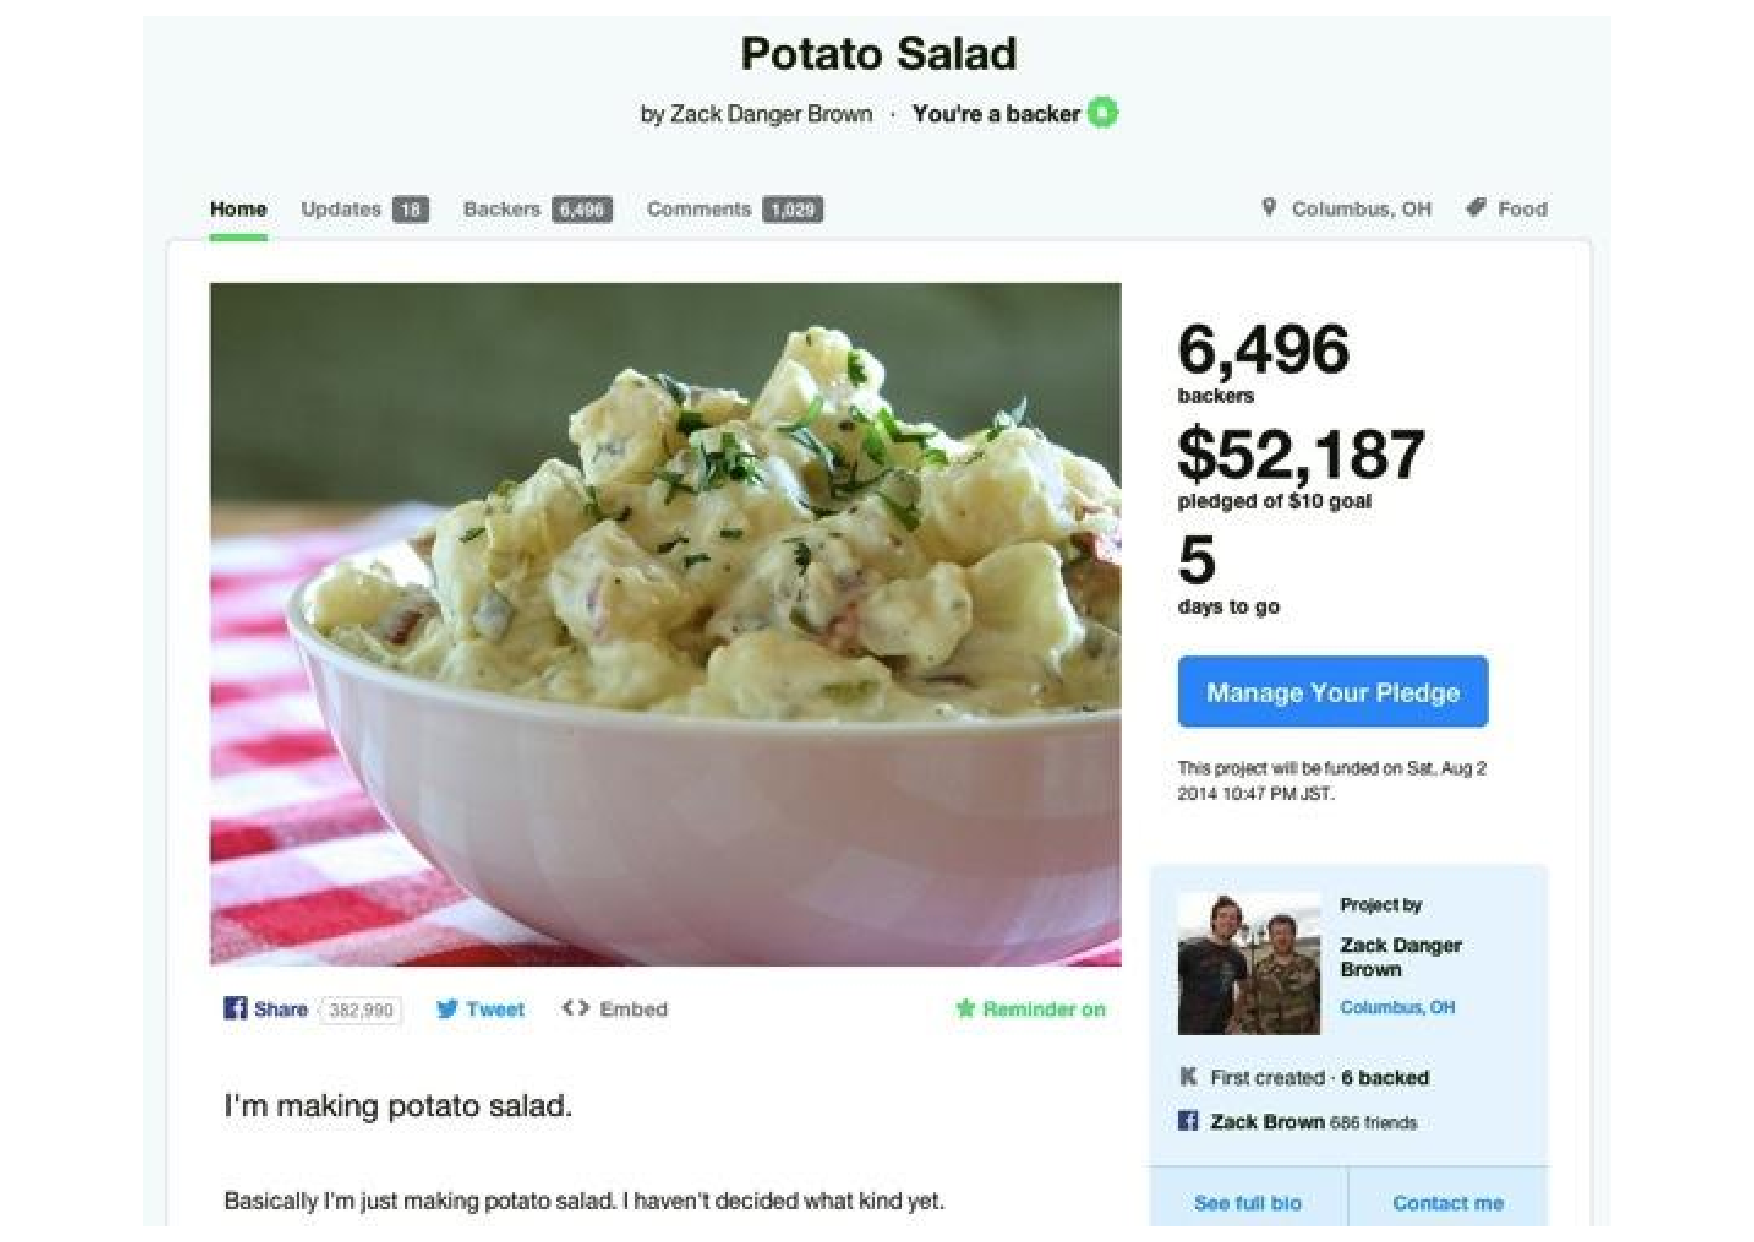
\includegraphics[width=13cm]{figure45.pdf}
\caption{ポテトサラダプロジェクト}\label{sannp}
\end{figure}

近年の例であるとOculus社が開発しているOculus社VRヘッドセットRiftが有名である.またOculus社はRiftのクラウドファンディングを成功した後にFacebook社に買収されてしまい,それが問題になっている.買収されてしまったことにより方針が変わってしまうことや,小さな会社が画期的なものを作るのを支援したかった人たちがFacebook社を批判する事態になっている.

\begin{figure}[H]
\centering
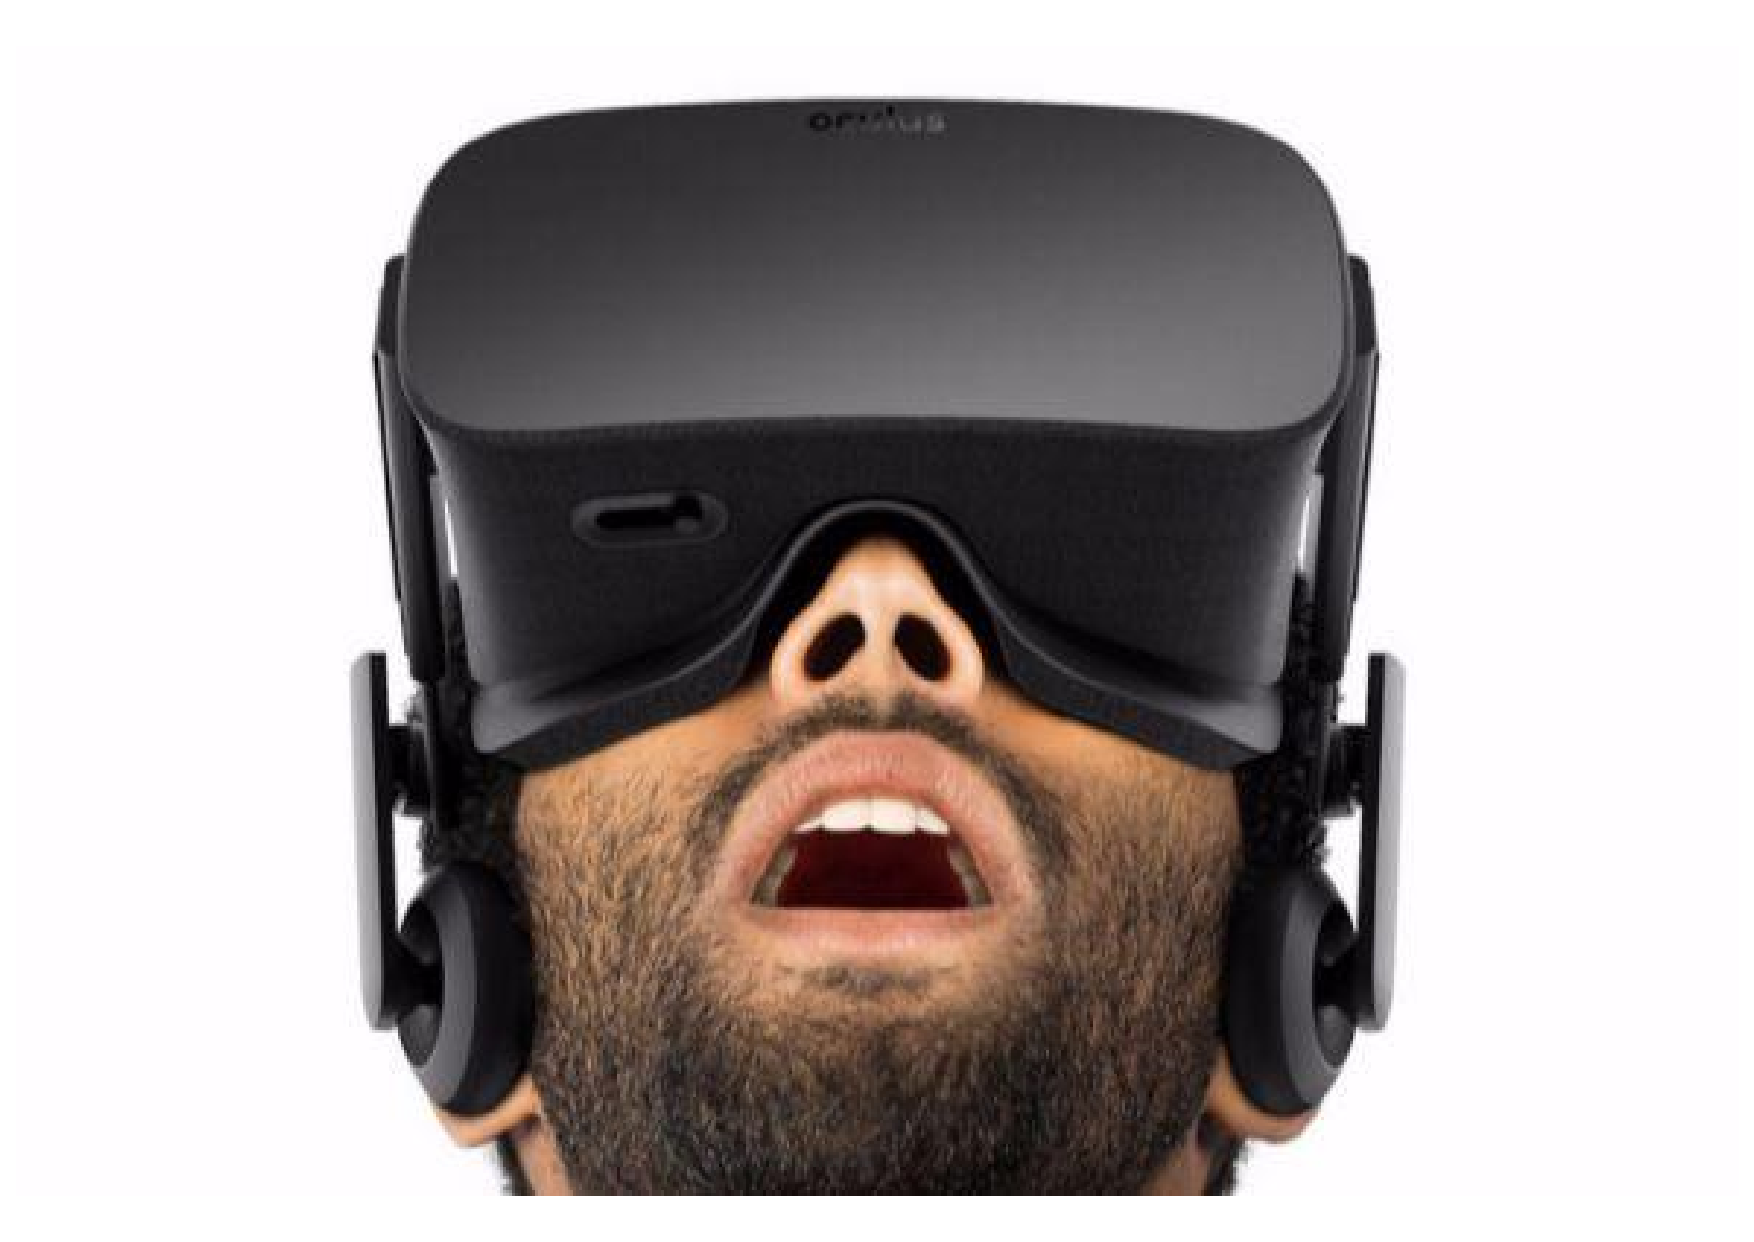
\includegraphics[width=10cm]{figure44.pdf}
\caption{Rift}\label{sannp}
\end{figure}

クラウドファンディングが成功しても開発が絶対にうまくいくとは限らず,お金を支払ったのに完成品をもらえないなど,クラウドファンディングに問題がないとは言い切れない.法改正やクラウドファンディングのルールが整うまでにまだ時間がかかると思われるが,画期的なアイディアや需要が見込める商品を実用化できるメリットは大きく規模は年々拡大している.

\chapter{データマイニングについて}
\section{本章の構成}
本章では,研究で使用するデータマイニングについて解説を記す.

\section{データマイニングとは}
データマイニングとは,1990年代中頃から用いられるようになった言語であり,大量のデータから統計学,パターン認識,人工知能などのデータ解析の技法を使い,大量のデータの中から知識を取り出す技術のことである.テキストを対象とするものをテキストマイニング,中でもウェブページを対象にしているものはウェブマイニングと呼ばれている.

\section{データマイニングの事例}
データマイニングの成功事例は,数多く報告されており,有名な話としておむつとビールの話しがある.
データマイニングにバスケット分析という,POSデータなどの取引データを分析する手法があり,「おむつを買った人はビールを買う傾向がある」という分析結果が1990代半ばから2000年台初めにかけてメディアや講演などでよく語られ,データマイニングという言葉と概念を有名にした.明確な答えはないが,かさばる紙おむつを父親に買いに行かせた時に,父親がついでにビールを買っていく推測と,深夜に30代の男性がおむつと一緒にビールを買っている傾向が発見されたことから,おむつを突然切らしてしまった母親に,父親がおむつの買い物を頼まれそのついでにビールを買っているのではないかという推測の2つが挙げられている.おむつとビールの売り場を近くにおいたことで店の売上向上につながった話もあり,データマイニングの結果から推測することで顧客の潜在的なニーズを引き出すことができる.

\section{データマイニングのツール}
大量のデータを扱うには,ツールが必要である.データマイニングのツールではSAS,SPSS,S言語が有名である.しかしデータマイニング機能を揃えたSAS,SPSS,S言語のパッケージは値段が高く,個人ユーザが簡単に使えるものではない,そこで現在普及してきているS言語並みの機能を持つフリーソフトRを今回はデータマイニングのツールとして用いることとする.
\chapter{R言語について}
\section{本章の構成}
本章では,研究で使用するR言語についてと利用方法について解説を記す.

\section{R言語とは}
ニュージーランドのオークランド大学の統計学科のRoss Ihakaと,アメリカのハーバード大学生物統計学科のRobert Gentleman によって開発が始められ,1997年からは多くの賛同者が加わり,開発が続けられているオープンソース方式のデータ解析・処理の専用ソフトである.\cite{rniyoru}
R言語の名前の由来は統計解析言語であるS言語の独自実装であるので,S言語の「一歩手前」の「R」という意味や,創設者二人の頭文字であるRに由来しているという説がある.\cite{toukei}R言語の特徴としては,汎用的な言語とはちがい,解析に特化した言語であるということ,またオープンソースであるため必要に応じて拡張機能を手に入れてくることで様々な用途に対応できることや,簡単なコマンドにより様々な機能が実現できることがあげられる.

\section{Rの導入}
R言語はUNIX,Windows,Macなど様々なOSで使用することが可能である.今回は,Windows版の導入方法を記す.
R言語の本家サイトにhttps://www.r-project.org/アクセスし,Downloadの項目にあるCRANをクリックする.
\begin{figure}[H]
\centering
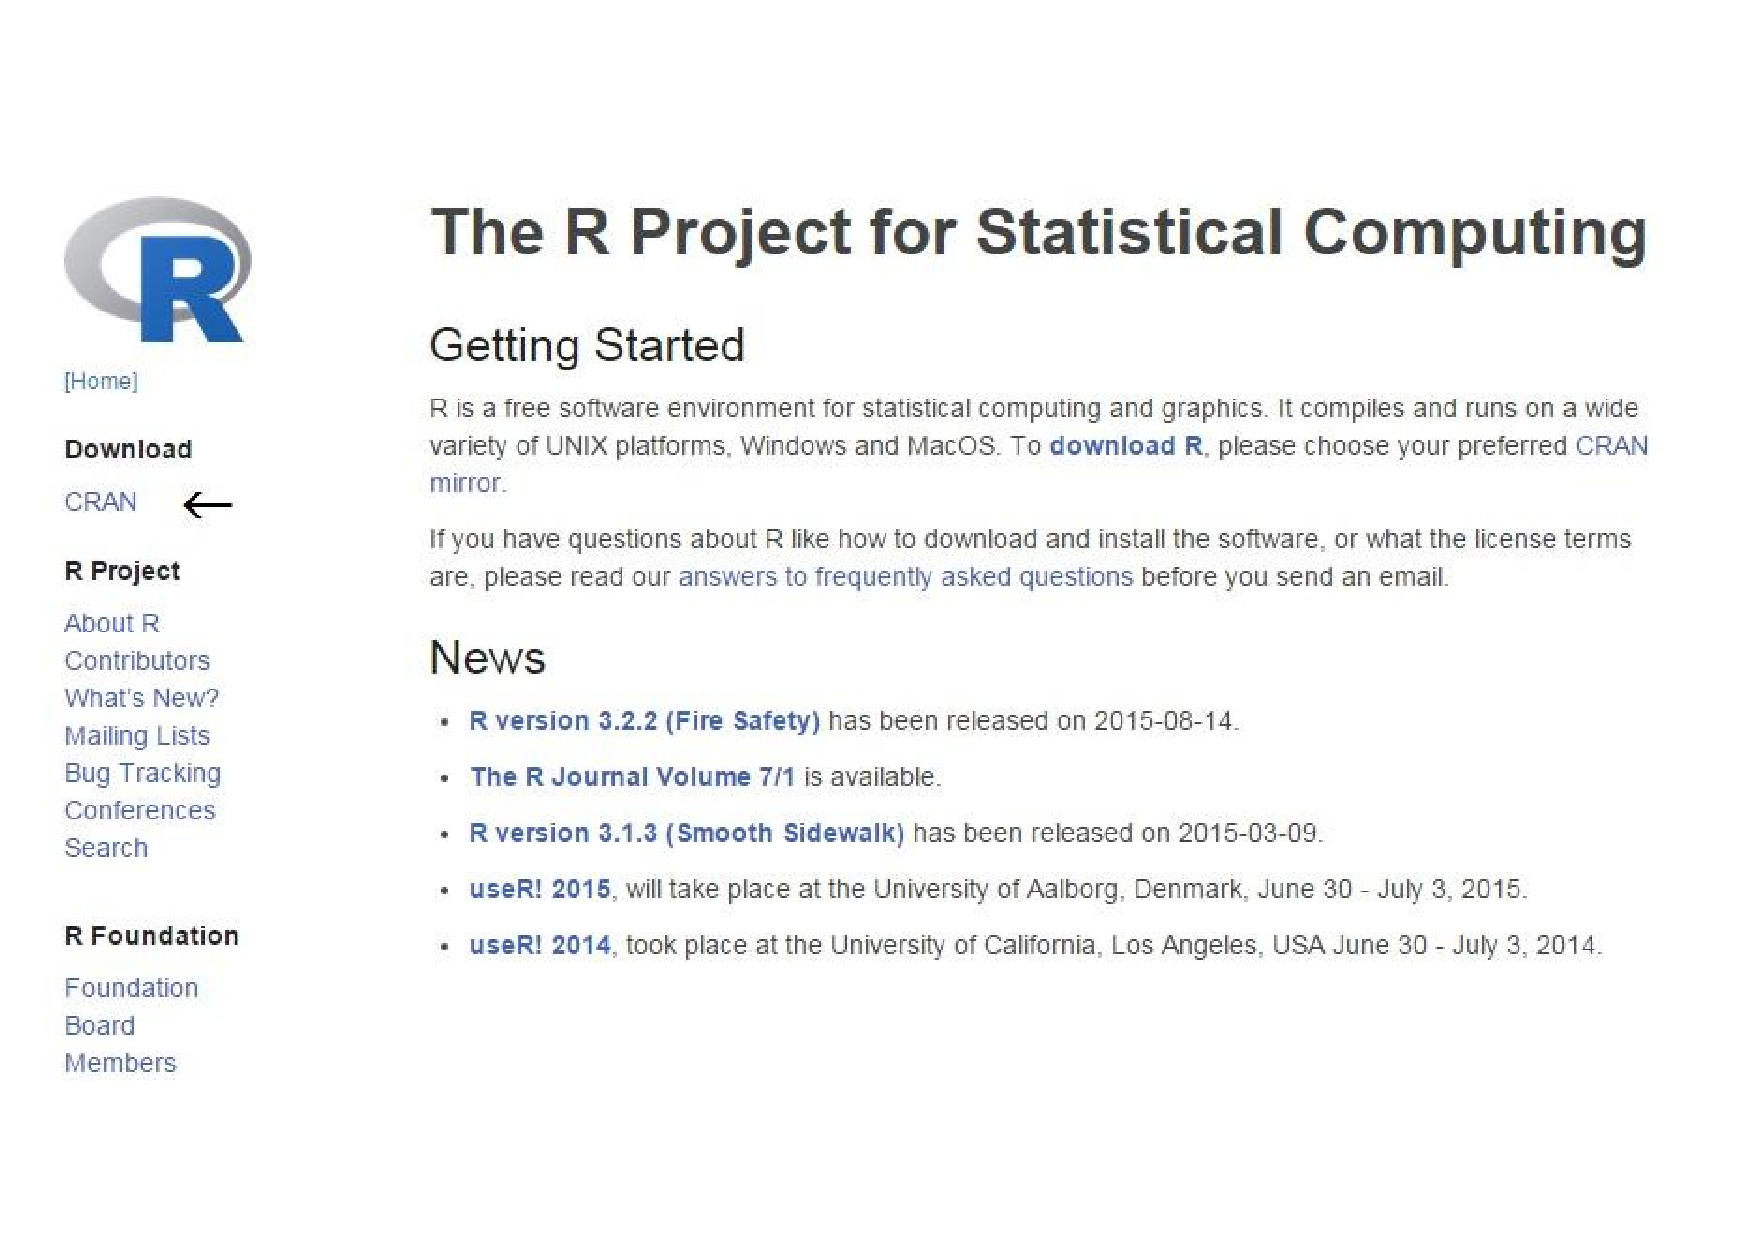
\includegraphics[width=13cm]{figure1.pdf}
\caption{Rインストール手順}\label{サンプル図}
\end{figure} 

「JAPAN」のリンクを探し,統計数理研究所か山形大学のRのミラーサイトをクリックする.

\begin{figure}[H]
\centering
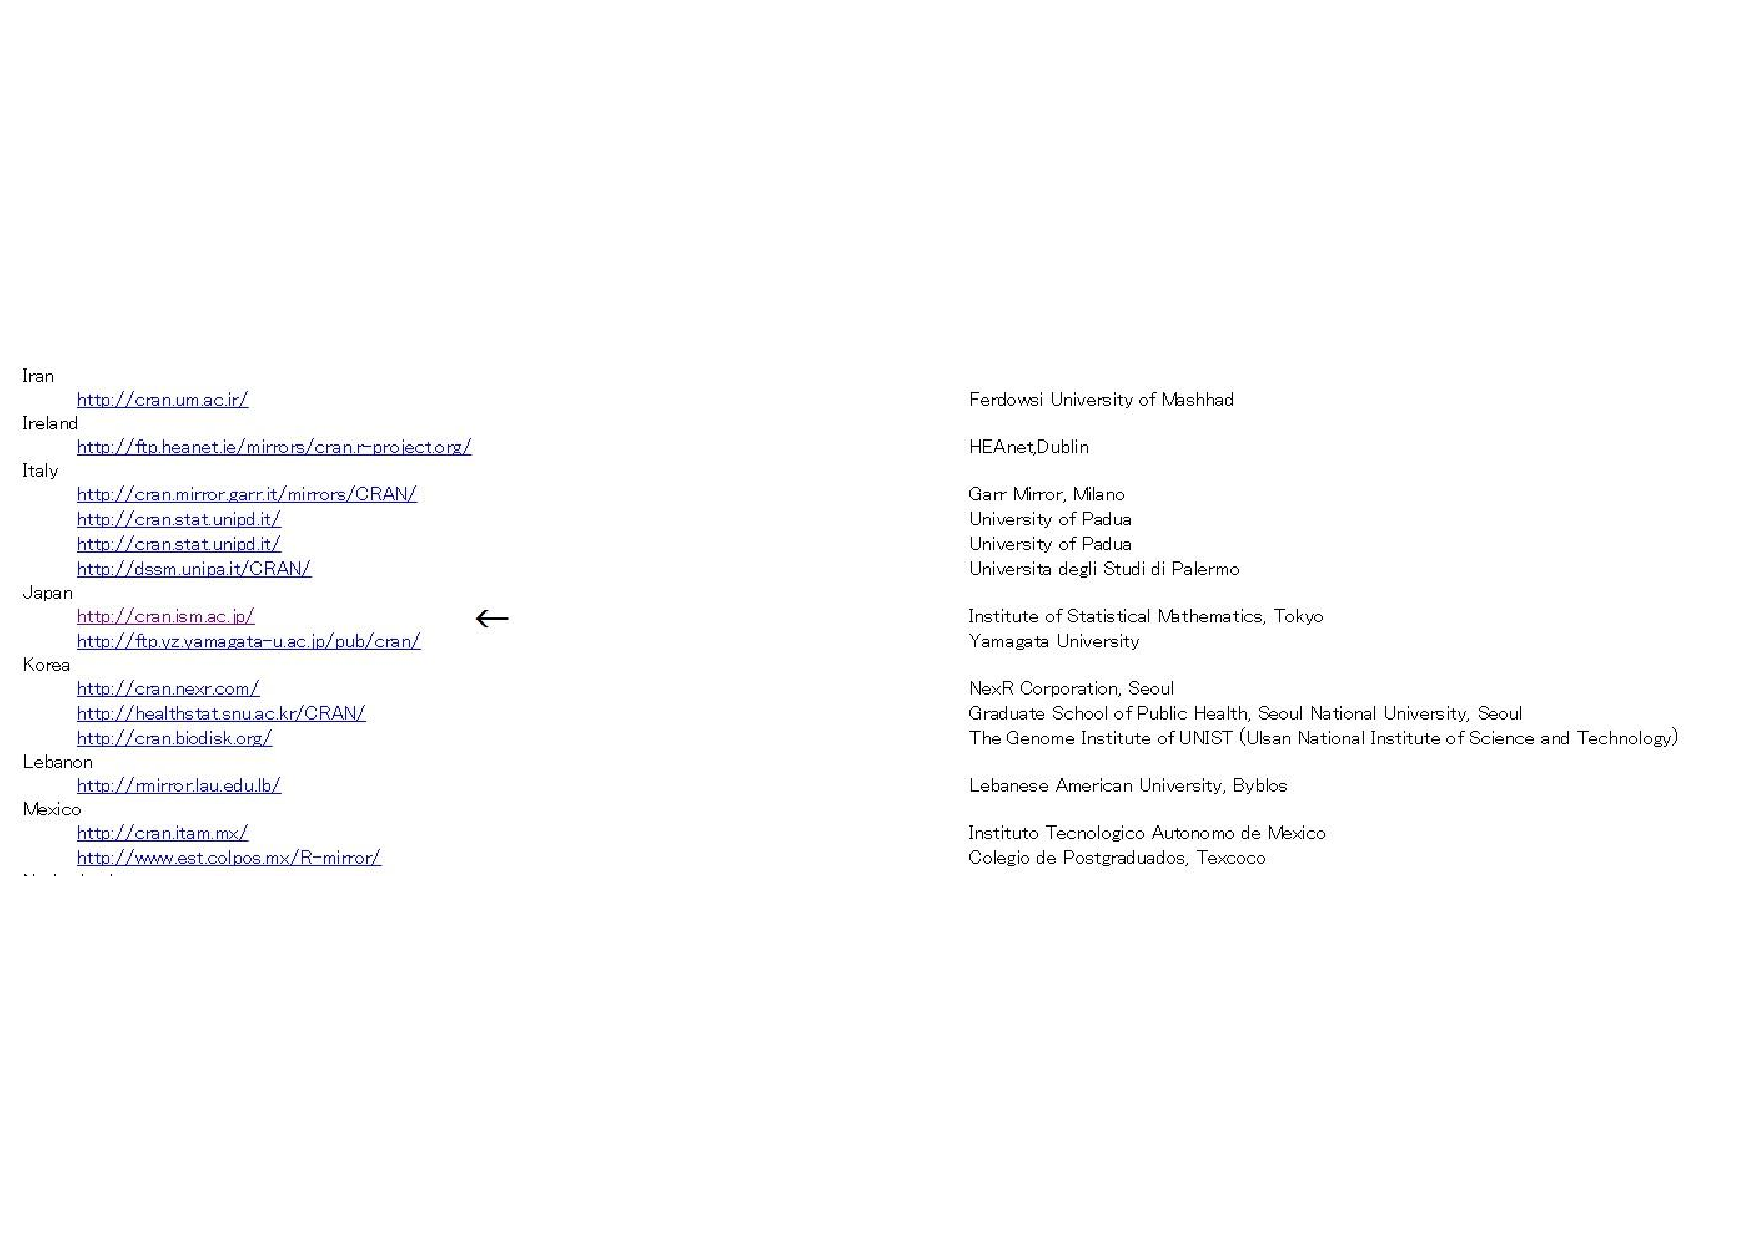
\includegraphics[width=13cm]{r1.pdf}
\caption{Rインストール手順2}\label{サンプル図}
\end{figure} 

画面上部にある「Download R for Windows」をクリックする.

\begin{figure}[H]
\centering
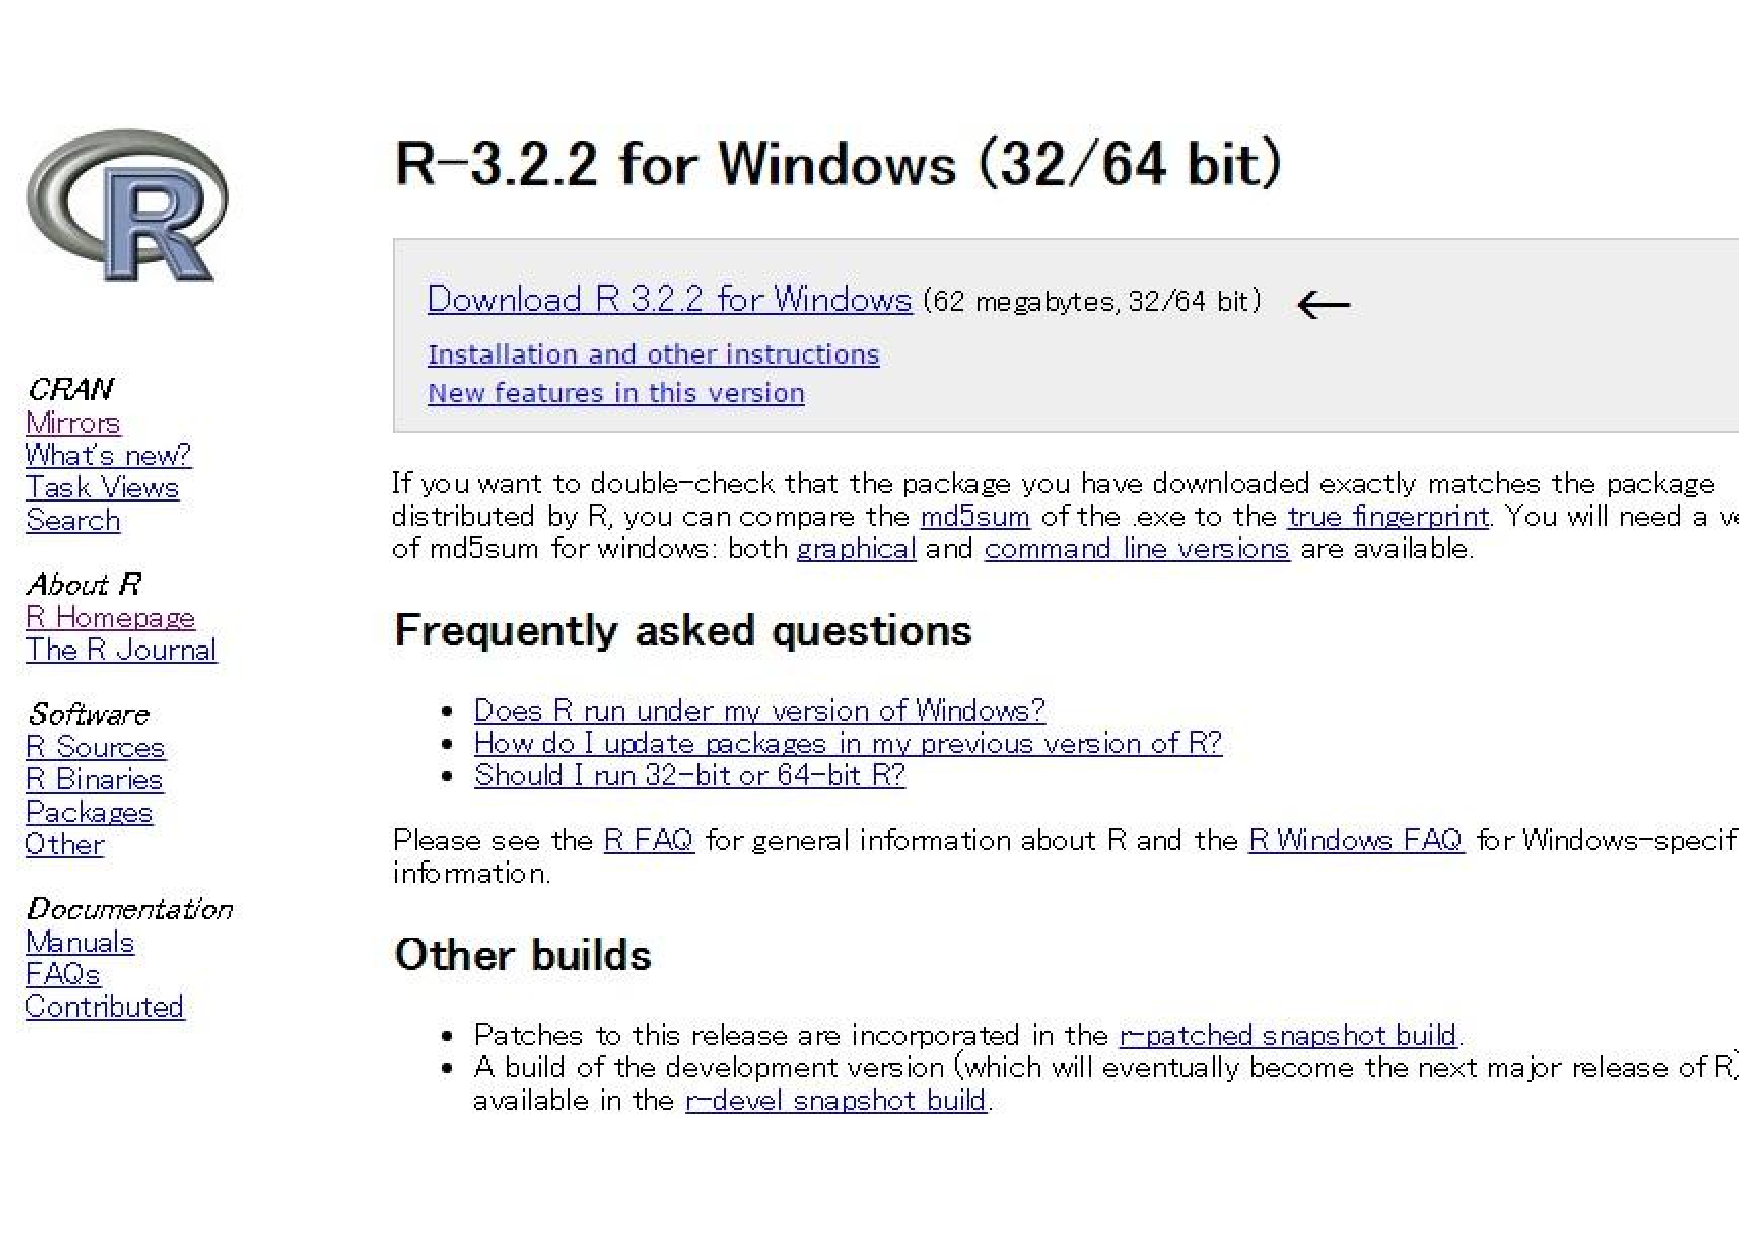
\includegraphics[width=13cm]{r2.pdf}
\caption{Rインストール手順3}\label{サンプル図}
\end{figure} 

リンクの一番上にあるbaseをクリックする.
「Download R 3.2.2 for Windows」をクリックするとDownloadが開始する.

\section{Rの起動と終了}
デスクトップ上のRのショートカットアイコンをクリックするか,「スタート」→「すべてのプログラム」→「R」のフォルダにあるRをクリックするとRGuiウィンドウが開く.
基本的にコンソール上で操作を行い,作成されたグラフはグラフィックウィンドウが出てきて表示がされる.Rを終了する際には,コンソールに「q()」または「quit()」と入力しEnterきーを 押すことで終了できる.
\begin{figure}[H]
\centering
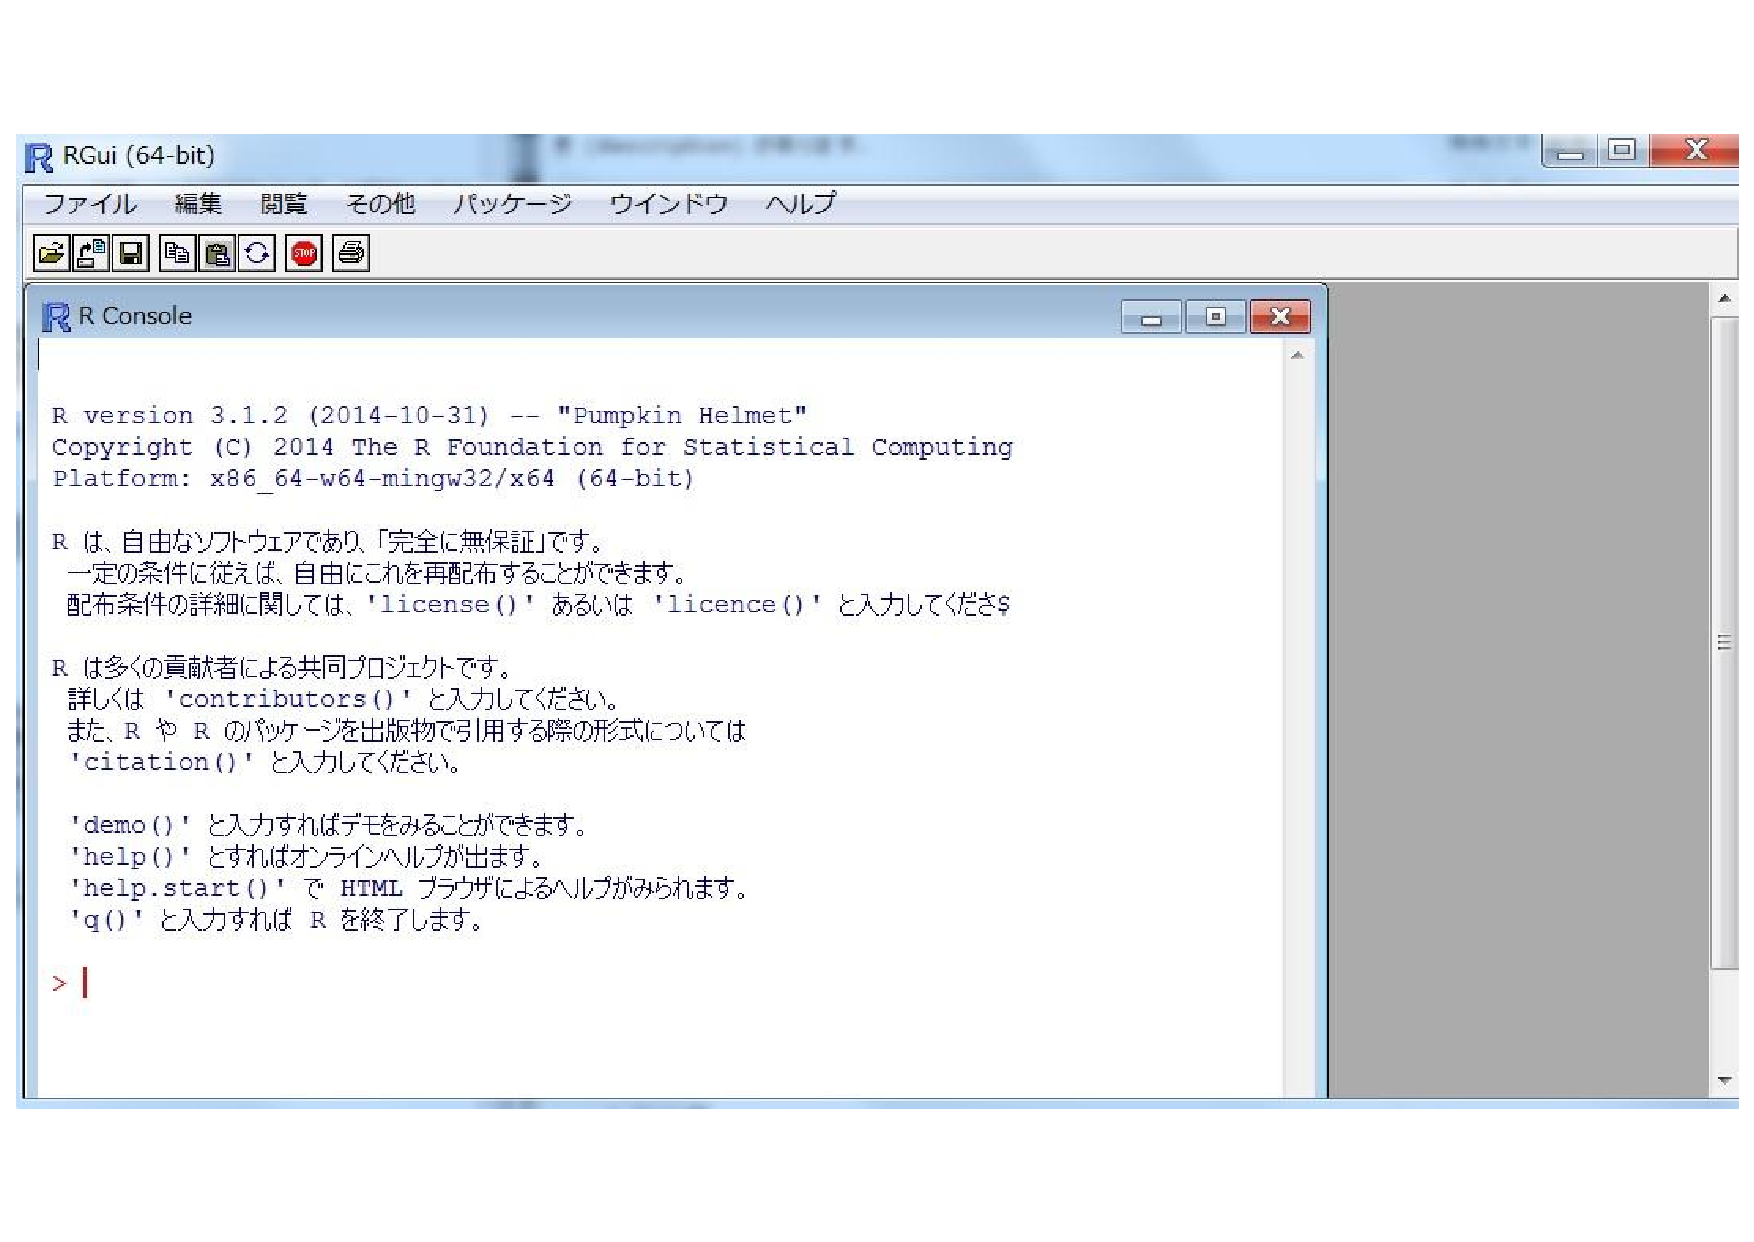
\includegraphics[width=13cm]{figure2.pdf}
\caption{Rインストール手順4}\label{sannp}
\end{figure}

\chapter{クローラーについて}
\section{本章の構成}
本章では,研究で使用したクローラーの作成方法について記す.

\section{クローラーとは}
ネット上の文章や画像などを周期的に所得し,自動的に保存するプログラムである.「ボット(Bot)」,スパイダー,ロボットとも呼ばれる.
今回はフリーソフトウェアであるwgetを利用し,作成したクローラーの説明を行う.

\section{wgetとは}
wgetとはウェブサーバーからコンテンツを取得するプログラムであり,多くのUNIXユーザーから利用されている.また多くの環境で利用可能であり,低速で不安定なインターネットでも確実に動作し,ダウンロードを行えるように設計されていることが特徴である.もしダウンロードが停止した場合,停止した箇所からダウンロードを継続するように試みてファイル全体が取得されるまで繰り返す.また再帰的にダウンロードを行うことが可能であるため,クローラーとして動作させることも可能であり,オプションを組みわせることでウェブサイトから画像や文章をダウンロードすることができる.
文法は「wget -オプション(オプション引数) URL」のように記述する.

\section{wgetオプション}
wgetを使いこなす上で重要であるオプションを解説していく.オプションは大文字と小文字で別の動作をするものがあり,使いたいオプションは大文字か小文字かきちんと確認しておくことが重要である.短縮形が無いオプションに関しては長いオプションで記述する.

\begin{table}[H]
  \begin{center}
    \caption{スタートアップ}
    \begin{tabular}{|l|c|} \hline
      コマンド名 & 解説  \\ \hline
      -V & wgetのバージョンを表示して終了  \\
      -h & オプション一覧のヘルプ  \\
      -b & スタート後にバックグラウンドに移行する.  \\
-e & 「.wgetrc形式のコマンドを実行する.」  \\ \hline
    \end{tabular}
  \end{center}
\end{table}

\begin{table}[H]
  \begin{center}
    \caption{ログと入力ファイル}
    \begin{tabular}{|l|c|} \hline
      コマンド名 & 解説  \\ \hline
      -o & ログをFILEに出力する  \\
      -a & メッセージをFILEに追記する  \\
      -d & デバック情報を表示する.  \\
-q & 何も表示しない  \\
-v & 冗長な出力をする(デフォルト)  \\
-nv & 冗長ではなくする  \\
--report-speed=TYPE & 帯域幅をTYPEで出力します.  \\
-i & FILEの中に指定されたURLをダウンロードする  \\
-F & 入力されたファイルをHTMLとして扱う  \\
-B & HTMLで入力されたファイル(-i -F)のリンクを設定したURLの相対URLとして扱う  \\
--configFILE & 設定ファイルを指定する  \\ \hline
    \end{tabular}
  \end{center}
\end{table}

\begin{table}[H]
  \begin{center}
    \caption{ダウンロード}
    \begin{tabular}{|l|c|} \hline
      コマンド名 & 解説  \\ \hline
      -t & リトライ回数の上限を設定(0は無制限)  \\
      -O & 接続を拒否されてもリトライする  \\
      -nc & FILEに文書を書き込む  \\
-c & 部分的にダウンロードしたファイルの続きから書き始める  \\
-N & ローカルにあるファイルよりも新しいファイルだけ取得する  \\
--no-use-server-timestamps & ローカル側のファイルスタンプにサーバーのものを使わない  \\
-S & サーバーの応答を表示する  \\
-T & 全てのタイムアウトをSECONDS秒に設定する  \\
--dns-timeout=SECS & DNS問い合わせのタイムアウトをSECS秒に設定する  \\
--connect-timeout=SECS & 接続タイムアウトをSECS秒に設定する  \\
--read-timeout=SECS & 読み込みタイムアウトをSECS秒に設定する  \\
-w & ダウンロード毎にSECONDS秒待つ  \\
--waitretry & リトライ毎に1~SECONDS秒待つ  \\
--no-proxy & プロクシを使わない  \\
-Q & ダウンロードするバイト数の上限を指定する  \\
--bind-address=ADDRESS & ローカルアドレスとしてADDRESS(ホスト名かIP)を使う  \\
--limit-rate=RATE & ダウンロード速度をRATEに制限する  \\
--no-dns-cache & DNSの問い合わせ結果をキャッシュしない  \\
-restrict-file-names=OS & OSが許しているファイル名に制限する  \\
--ignore-case & ファイル名,ディレクトリ名の比較で大文字小文字を無視する  \\
-4 & IPv4だけを使う  \\
-6 & IPv6だけを使う  \\
--prefer-family=FAMILY & 指定したファミリ(IP6v,IPv4,none)で最初に接続する  \\
--user=USER & ftp,httpのユーザー名を指定する  \\
--password=PASSWORD & ftp,httpのパスワードを指定する  \\
--ask-password & パスワードを別途入力する  \\
--no-iri & IRIサポートを使わない  \\
--local-encoding=ENC & 指定したENCをIRIのローカルエンコーディングにする  \\
--remote-encodging=ENC & 指定したENCをデフォルトのリモートエンコーディングにする  \\
--unlink & 上書きする前にファイルを削除する  \\ \hline
    \end{tabular}
  \end{center}
\end{table}

\begin{table}[H]
  \begin{center}
    \caption{ディレクトリ}
    \begin{tabular}{|l|c|} \hline
      コマンド名 & 解説  \\ \hline
-nd & ディレクトリを作らない \\
-x & ディレクトリを強制的に作る \\
-nH & ホスト名のディレクトリを作らない \\
--protocol-directories & プロトコル名のディレクトリを作る \\
-P & ファイルをPREFIX以下に保存する \\
--cut-dirs=NUMBER & リモートディレクトリ名の NUMBER 階層分を無視する \\ \hline
    \end{tabular}
  \end{center}
\end{table}


\begin{table}[H]
  \begin{center}
    \caption{HTTP オプション}
    \begin{tabular}{|l|c|} \hline
      コマンド名 & 解説  \\ \hline
 --http-user=USER & http ユーザ名として USER を使う \\
       --http-password=PASS & http パスワードとして PASS を使う \\
       --no-cache & サーバがキャッシュしたデータを許可しない \\
       --default-page=NAME & デフォルトのページ名を NAME に変更します. \\
  -E & HTML/CSS 文書は適切な拡張子で保存する \\
       --ignore-length & Content-Lengthヘッダを無視する \\
       --header=STRING & 送信するヘッダに STRING を追加する \\
       --max-redirect & ページで許可する最大転送回数 \\
       --proxy-user=USER & プロクシユーザ名として USER を使う \\
       --proxy-password=PASS & プロクシパスワードとして PASS を使う \\
       --referer=URL & Referer を URL に設定する \\
       --save-headers & HTTP のヘッダをファイルに保存する \\
  -U & User-Agent として Wget/VERSION ではなく AGENT を使う \\
       --no-http-keep-alive & HTTP の keep-alive (持続的接続) 機能を使わない \\
       --no-cookies & クッキーを使わない \\
       --load-cookies=FILE & クッキーを FILE から読みこむ \\
       --save-cookies=FILE & クッキーを FILE に保存する \\
       --keep-session-cookies & セッションだけで用いるクッキーを保持する \\
       --post-data=STRING & POST メソッドを用いて STRING を送信する \\
       --post-file=FILE & POST メソッドを用いて FILE の中味を送信する \\
       --content-disposition & Content-Disposition ヘッダがあればローカルのファイル名として用いる \\ 
       --auth-no-challenge & サーバからのチャレンジを待たずに、Basic認証の情報を送信します。 \\ \hline
    \end{tabular}
  \end{center}
\end{table}

\begin{table}[H]
  \begin{center}
    \caption{HTTPS (SSL/TLS) オプション}
    \begin{tabular}{|l|c|} \hline
      コマンド名 & 解説  \\ \hline
 --secure-protocol=PR & セキュアプロトコルを選択する (auto, SSLv2, SSLv3, TLSv1) \\
       --no-check-certificate & サーバ証明書を検証しない \\
       --certificate=FILE & クライアント証明書として FILE を使う \\
       --certificate-type=TYPE & クライアント証明書の種類を TYPE (PEM, DER) に設定する \\
       --private-key=FILE & 秘密鍵として FILE を使う \\
       --private-key-type=TYPE & 秘密鍵の種類を TYPE (PEM, DER) に設定する \\
       --ca-certificate=FILE & CA 証明書として FILE を使う \\
       --ca-directory=DIR & CA のハッシュリストが保持されているディレクトリを指定する \\
       --random-file=FILE & SSL PRNG の初期化データに使うファイルを指定する \\
       --egd-file=FILE & EGD ソケットとして FILE を使う \\ \hline
    \end{tabular}
  \end{center}
\end{table}

\begin{table}[H]
  \begin{center}
    \caption{FTP オプション}
    \begin{tabular}{|l|c|} \hline
      コマンド名 & 解説  \\ \hline
 --ftp-user=USER & ftp ユーザとして USER を使う \\
       --ftp-password=PASS & ftp パスワードとして PASS を使う \\
       --no-remove-listing & .listingファイルを削除しない \\
       --no-glob & FTP ファイル名のグロブを無効にする \\
       --no-passive-ftp & passive転送モードを使わない \\
       --retr-symlinks & 再帰取得中に、シンボリックリンクでリンクされた先のファイルを取得する \\ \hline
    \end{tabular}
  \end{center}
\end{table}

\begin{table}[H]
  \begin{center}
    \caption{再起ダウンロード}
    \begin{tabular}{|l|c|} \hline
      コマンド名 & 解説  \\ \hline
  -r & 再帰ダウンロードを行う \\
  -l & 再帰時の階層の最大の深さを NUMBER に設定する (0 で無制限) \\
--delete-after & ダウンロード終了後、ダウンロードしたファイルを削除する \\
  -k & HTML や CSS 中のリンクをローカルを指すように変更する \\
  -K & リンク変換前のファイルを .orig として保存する \\
  -m & -N -r -l 0 --no-remove-listing の省略形 \\
  -p & HTML を表示するのに必要な全ての画像等も取得する \\
--strict-comments & HTML 中のコメントの処理を厳密にする \\ \hline
    \end{tabular}
  \end{center}
\end{table}

\begin{table}[H]
  \begin{center}
    \caption{再起ダウンロード時のフィルタ}
    \begin{tabular}{|l|c|} \hline
      コマンド名 & 解説  \\ \hline
  -A & ダウンロードする拡張子をコンマ区切りで指定する \\
  -R & ダウンロードしない拡張子をコンマ区切りで指定する \\
  -D & ダウンロードするドメインをコンマ区切りで指定する \\
--exclude-domains=LIST & ダウンロードしないドメインをコンマ区切りで指定する \\
--follow-ftp=HTML & 文書中の FTP リンクも取得対象にする \\
--follow-tags=LIST & 取得対象にするタグ名をコンマ区切りで指定する \\
--ignore-tags=LIST & 取得対象にしないタグ名をコンマ区切りで指定する \\
  -H & 再帰中に別のホストもダウンロード対象にする \\
  -L & 相対リンクだけ取得対象にする \\
  -I & 取得対象にするディレクトリを指定する \\
  -X & 取得対象にしないディレクトリを指定する \\
  -np & 親ディレクトリを取得対象にしない \\ \hline
 \end{tabular}
  \end{center}
\end{table}



\chapter{クローラーの導入}
\section{本章の構成}
本章ではクローラーの調査環境として利用するUbuntuとクローラーの運用について解説を記す.

\section{Ubuntuについて}
Ubuntu(ウブントゥ) とは、コミュニティ により開発されているオペレーティングシステムです。ラップトップ、デスクトップ、そしてサーバーに利用することができます。Ubuntuには、家庭・学校・職場で必要とされるワープロやメールソフトから、サーバーソフトウェアやプログラミングツールまで、あらゆるソフトウェアが含まれています。

Ubuntuは現在、そして将来に渡って無償で提供されます。ライセンス料を支払う必要はありません。Ubuntuをダウンロードすれば、友達や家族と、あるいは学校やビジネスに、完全に無料で利用できます。

私たちは、新しいデスクトップおよびサーバーを6ヶ月ごとにリリースすることを宣言しています。これにより、オープンソースの世界が提供する最新の優れたアプリケーションを常に利用できるようにしています。

Quantal Quetzal 12.10 2012年10月18日 2014年4月
Ubuntuは、セキュリティに配慮して設計されています。デスクトップおよびサーバーの無償セキュリティアップデートが、少なくとも9ヶ月間に渡って提供されます。長期サポート(LTS)版を利用すれば、5年間に渡りセキュリティアップデート提供されます。もちろん、LTS版を利用するために追加の費用は必要ありません。すべての人が無償という同じ条件で、私たちの精一杯の成果を利用することができます。Ubuntuを新しいバージョンにアップグレードする場合も、常に無償です。

Ubuntuのインストールイメージにはデスクトップ環境がひと通り含まれています。さらに、オンラインでソフトウェアを追加することができます。

グラフィカルインストーラにより、素早く簡単にインストールして使い始めることができます。標準的なインストールにかかる時間は10〜20分未満です。十分に高速な環境であれば、インストールが5分程度で終了することもあります。

一度システムをインストールすれば、インターネット、ドローイング、グラフィックス、そしてゲームといったアプリケーションがすぐに使えるようになります。

Ubuntuサーバーでは、ユーザーがセットアップしたものだけが動作し、それ以外はインストールされません。\cite{ubuntu}

\section{Ubuntuの導入}
調査環境として利用するUbuntuの導入を記す.現在Ubuntuは15.04までリリースされているが,利用者が多く,エラーが出た場合でも対応しやすい12.04を利用する.また仮想化ソフトのVirtualBox上で動作させること前提に解説を進める.初めに,Ubuntuの公式サイトにアクセスし,画面中央部のUbuntuのダウンロードを選択する.

\begin{figure}[H]
\centering
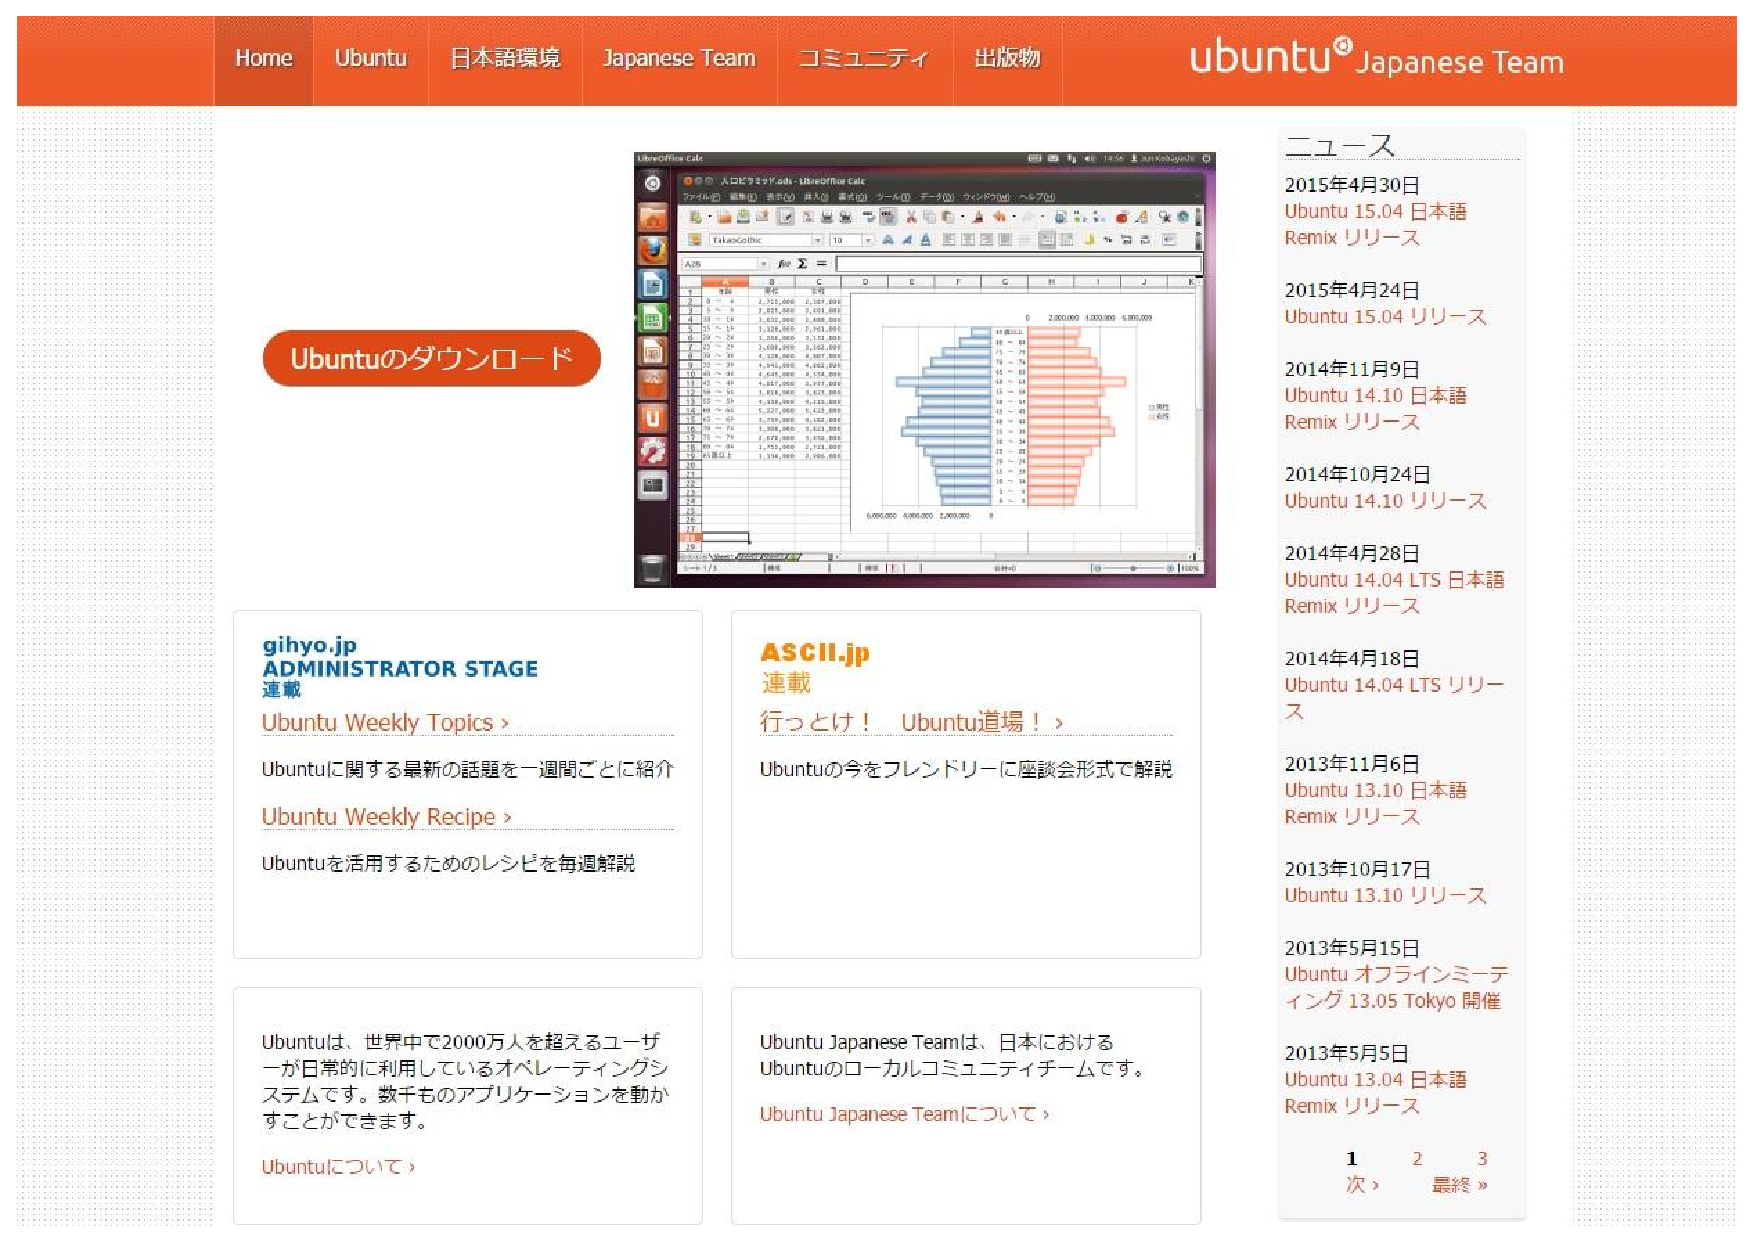
\includegraphics[width=13cm]{figure8.pdf}
\caption{Ubuntuの導入}\label{sannp}
\end{figure}

使用しているコンピューターのメインOSをUbuntuに変更するのであれば,「日本語Remixイメージのダウンロード」今回のようにVirtualBox上で動作させる場合には「日本語Remix仮想ハードディスクイメージのダウンロード」を選択する.

\begin{figure}[H]
\centering
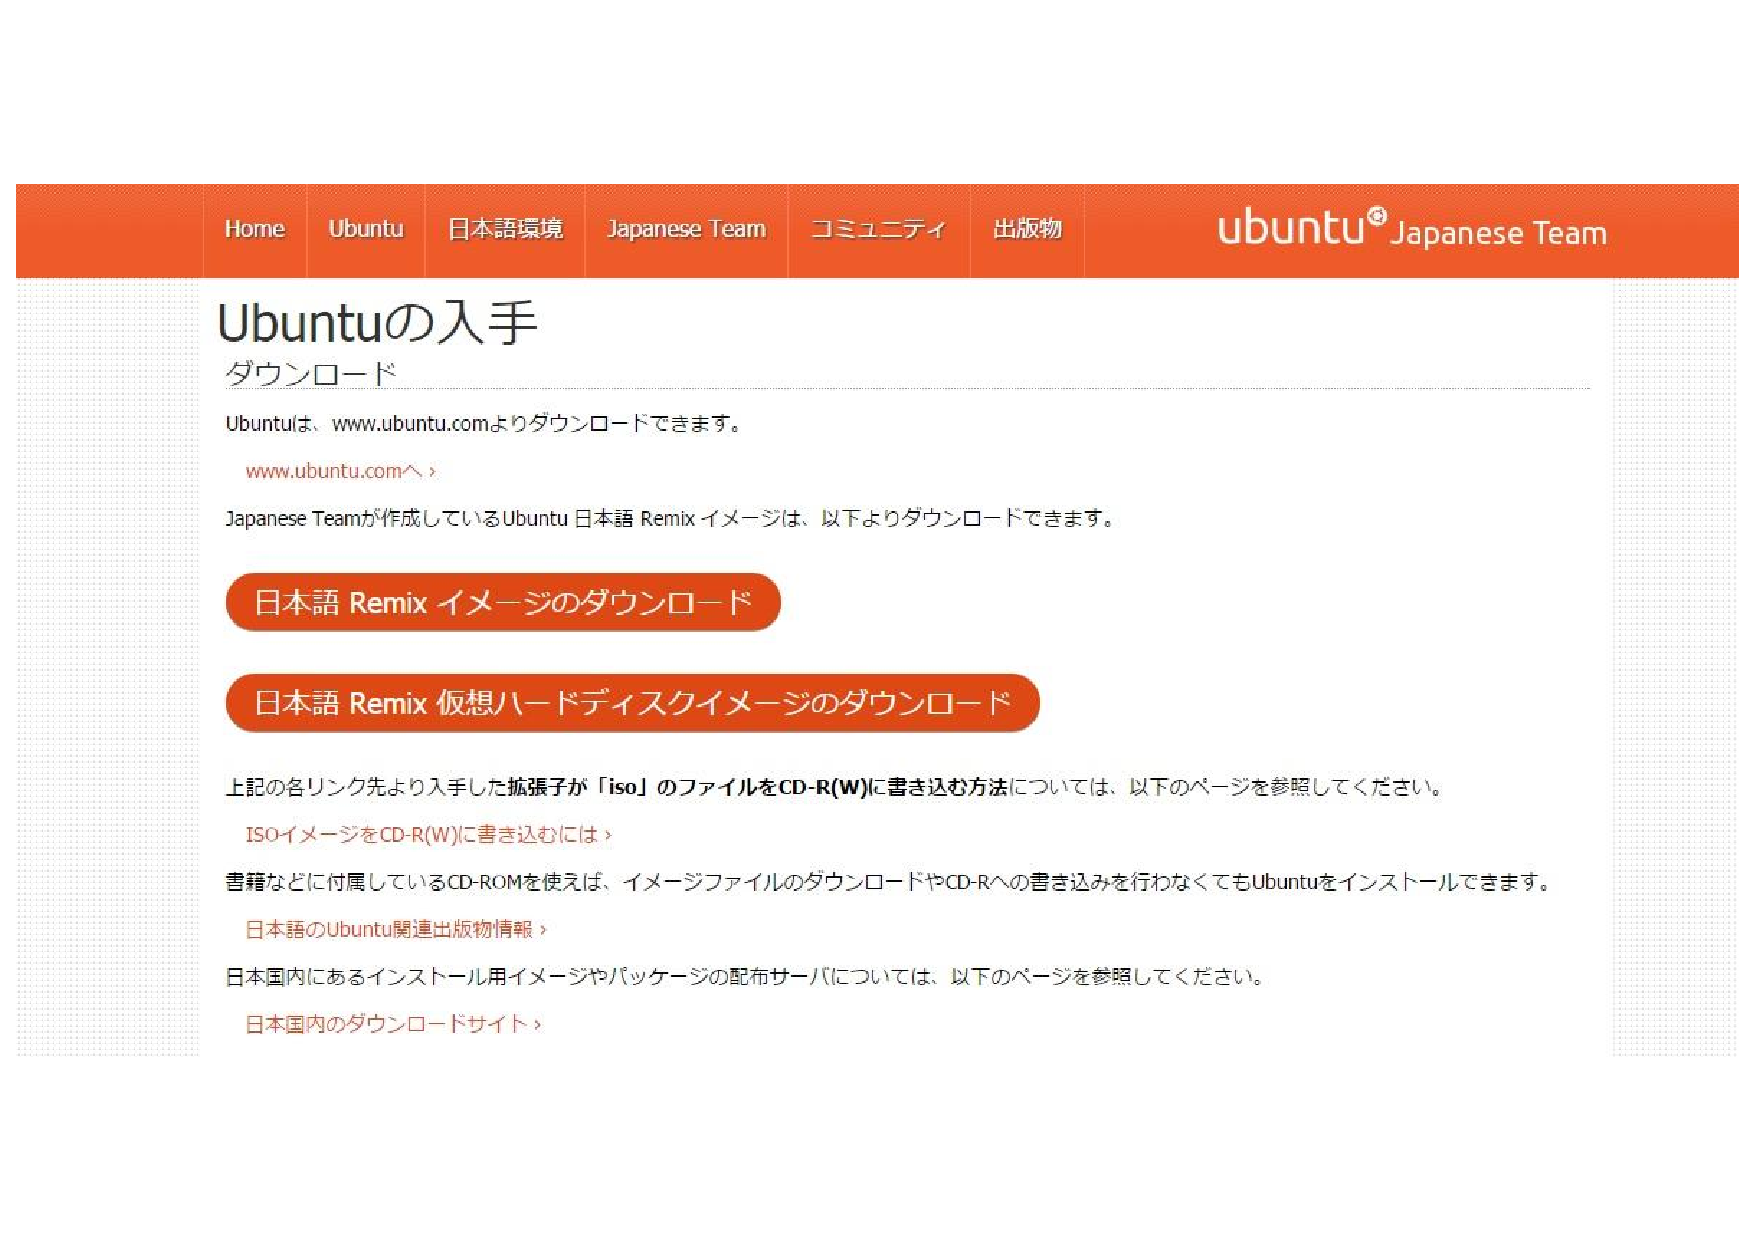
\includegraphics[width=13cm]{figure9.pdf}
\caption{Ubuntuの導2}\label{sannp}
\end{figure}

画面上部のUbuntu 12.04 LTSの項目内にある,「ubuntu-ja-12.04-desktop-i386-vhd.zip」を選択し,ダウンロードを行う.

\begin{figure}[H]
\centering
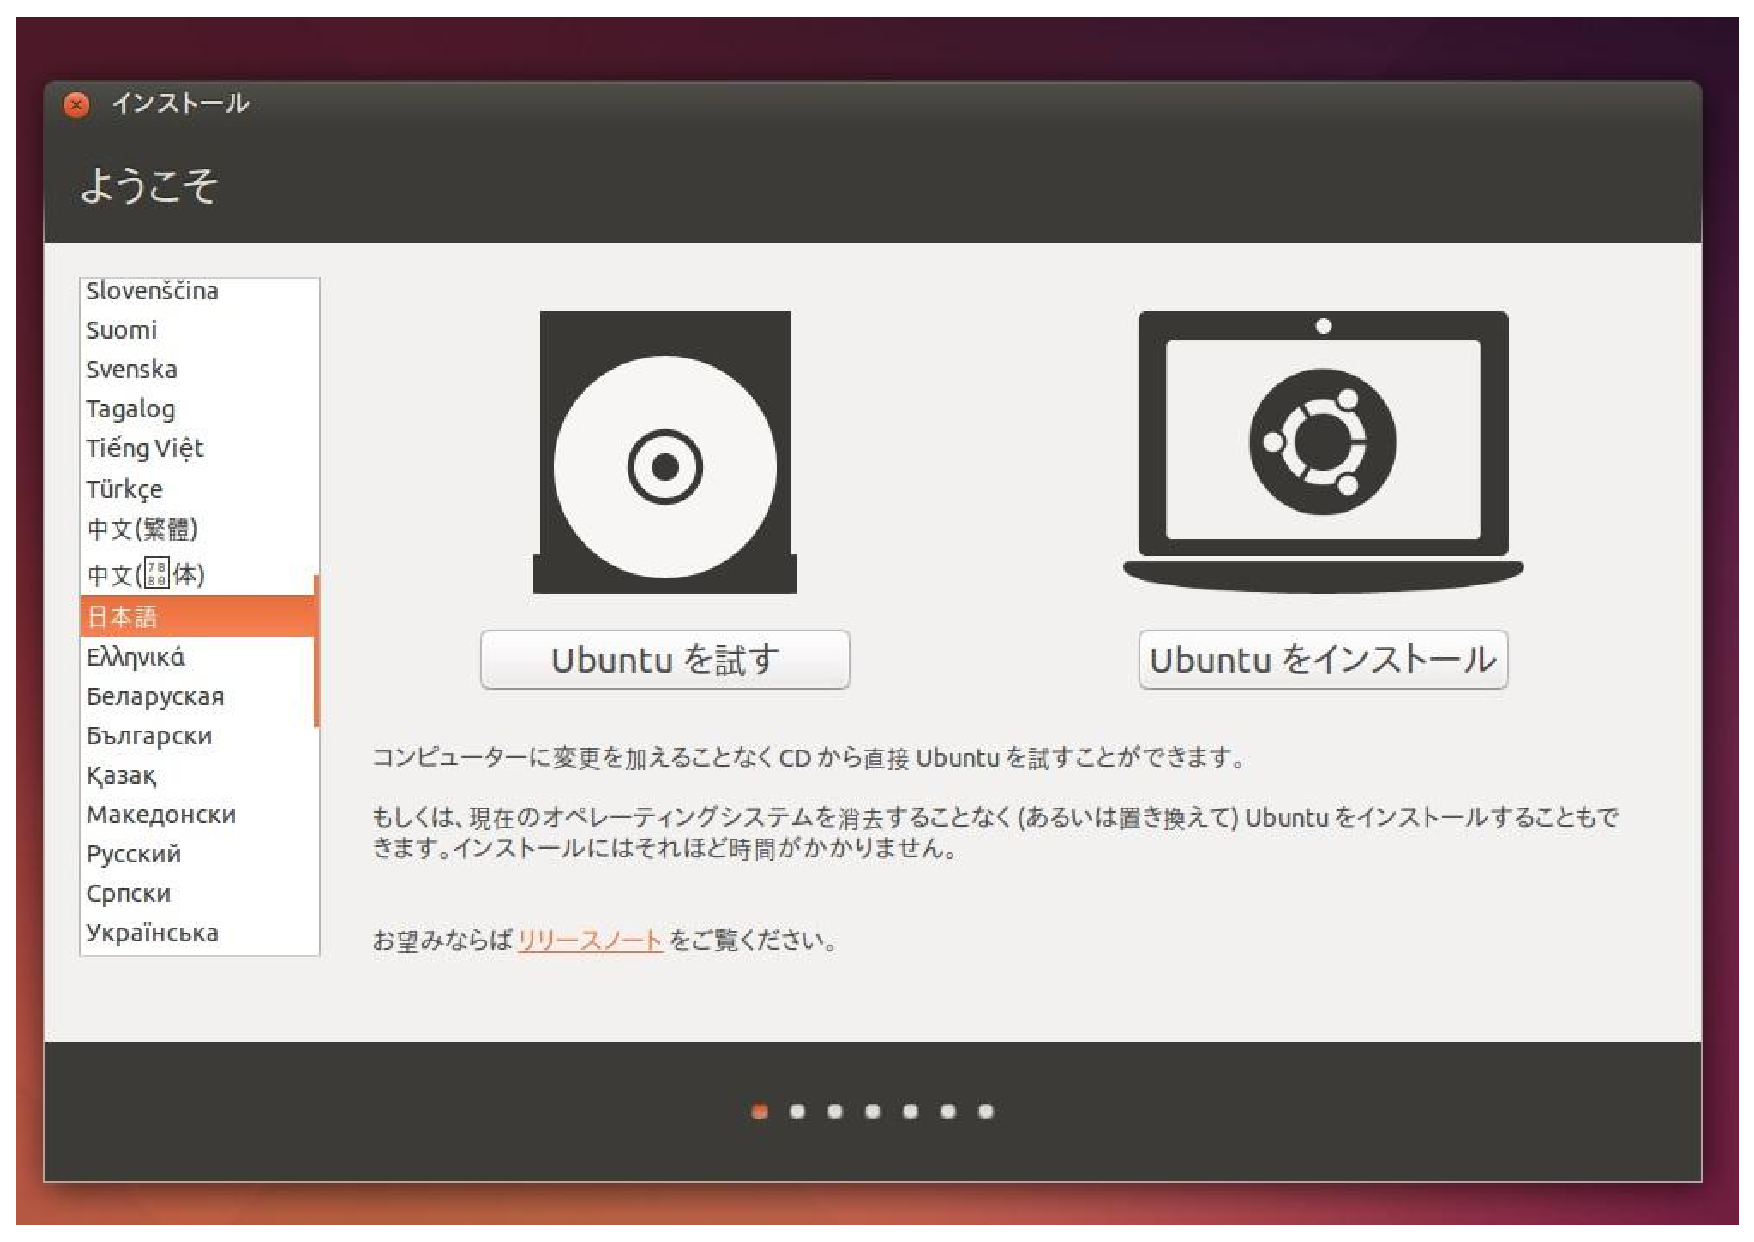
\includegraphics[width=13cm]{ins.pdf}
\caption{Ubuntuの導入3}\label{sannp}
\end{figure}

VirtualBox上で新規仮想マシンを作成し,Ubuntuのインストールを進める.自家国語を選択し,ubuntuをインストールを選択する.

\begin{figure}[H]
\centering
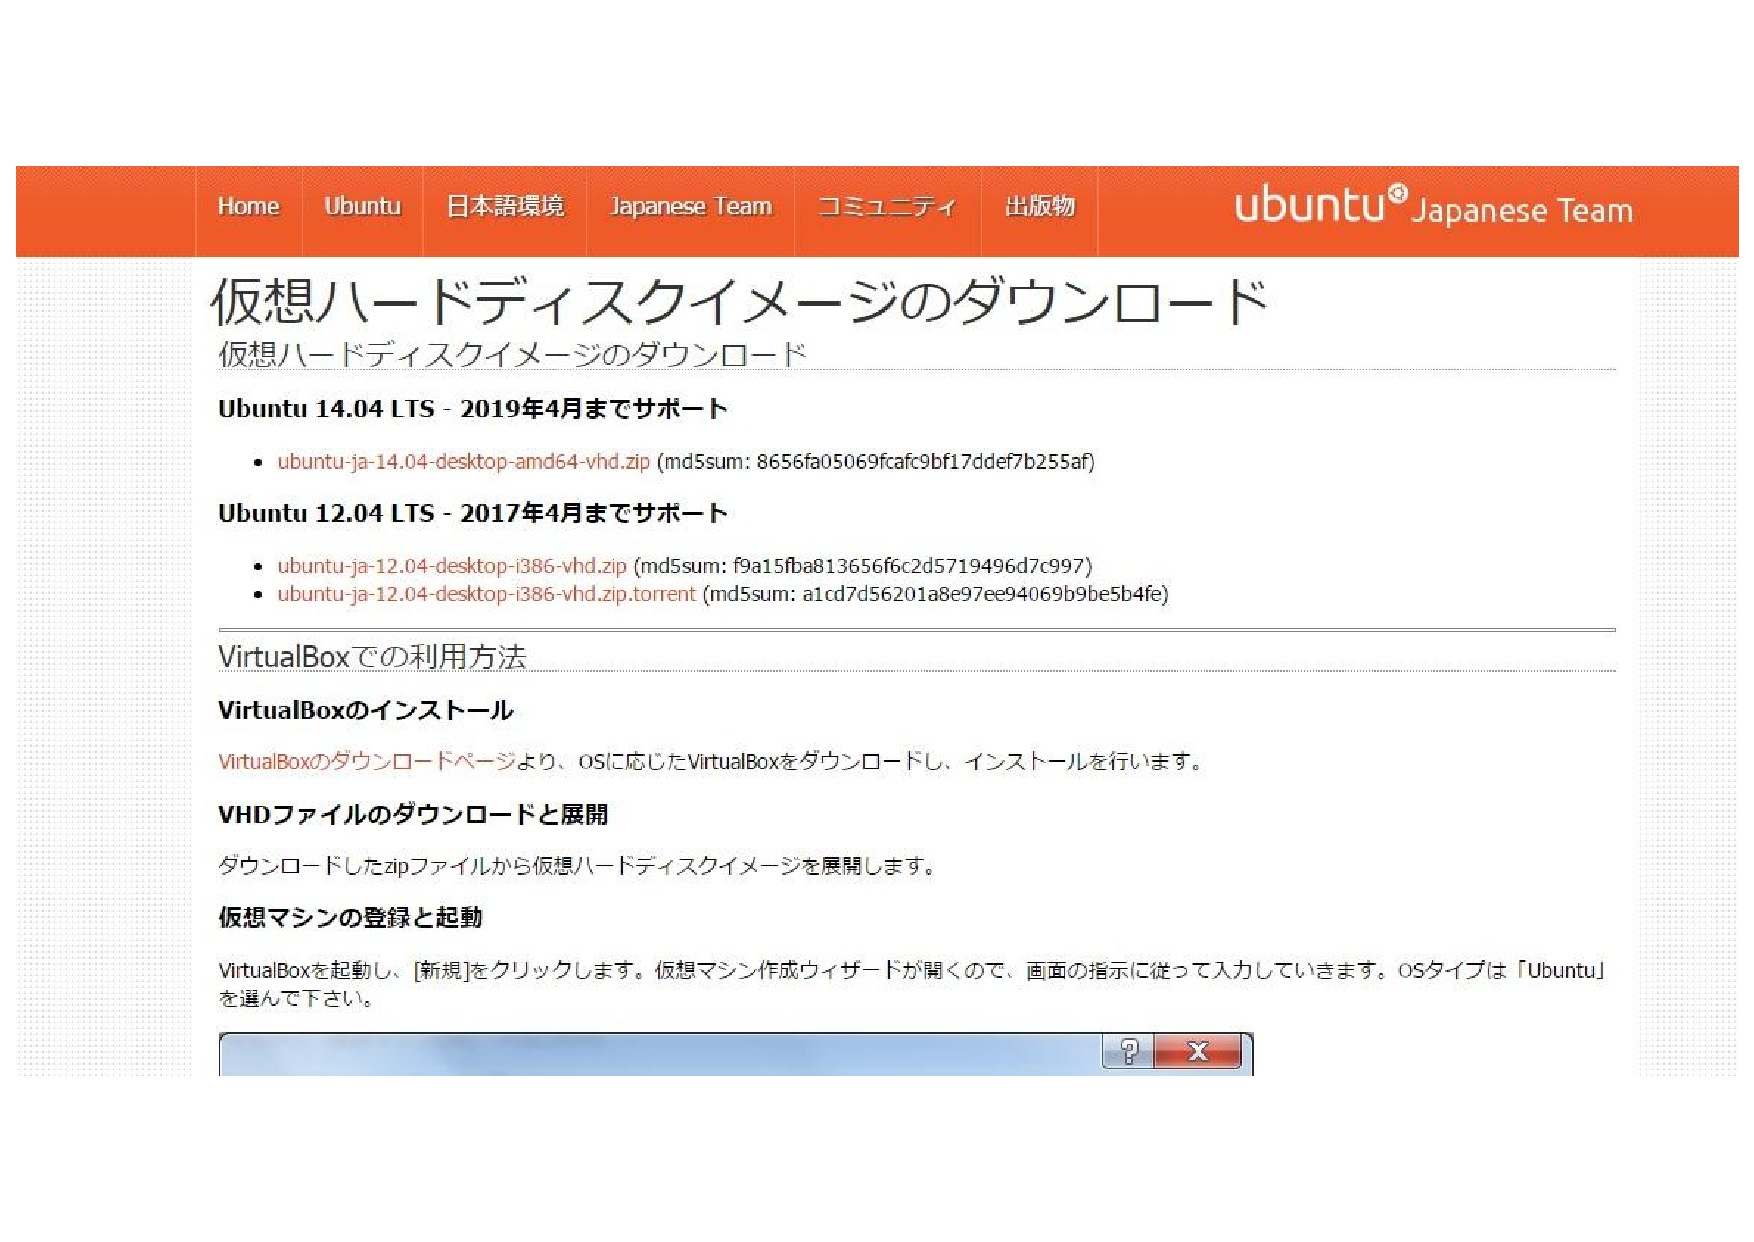
\includegraphics[width=13cm]{figure10.pdf}
\caption{Ubuntuの導入4}\label{sannp}
\end{figure}

次に自分の国を設定する.時刻に関わる設定のため研究を行う国で設定を行う.続けるを選択し,次の画面でキーボードレイアウトを行う.

\begin{figure}[H]
\centering
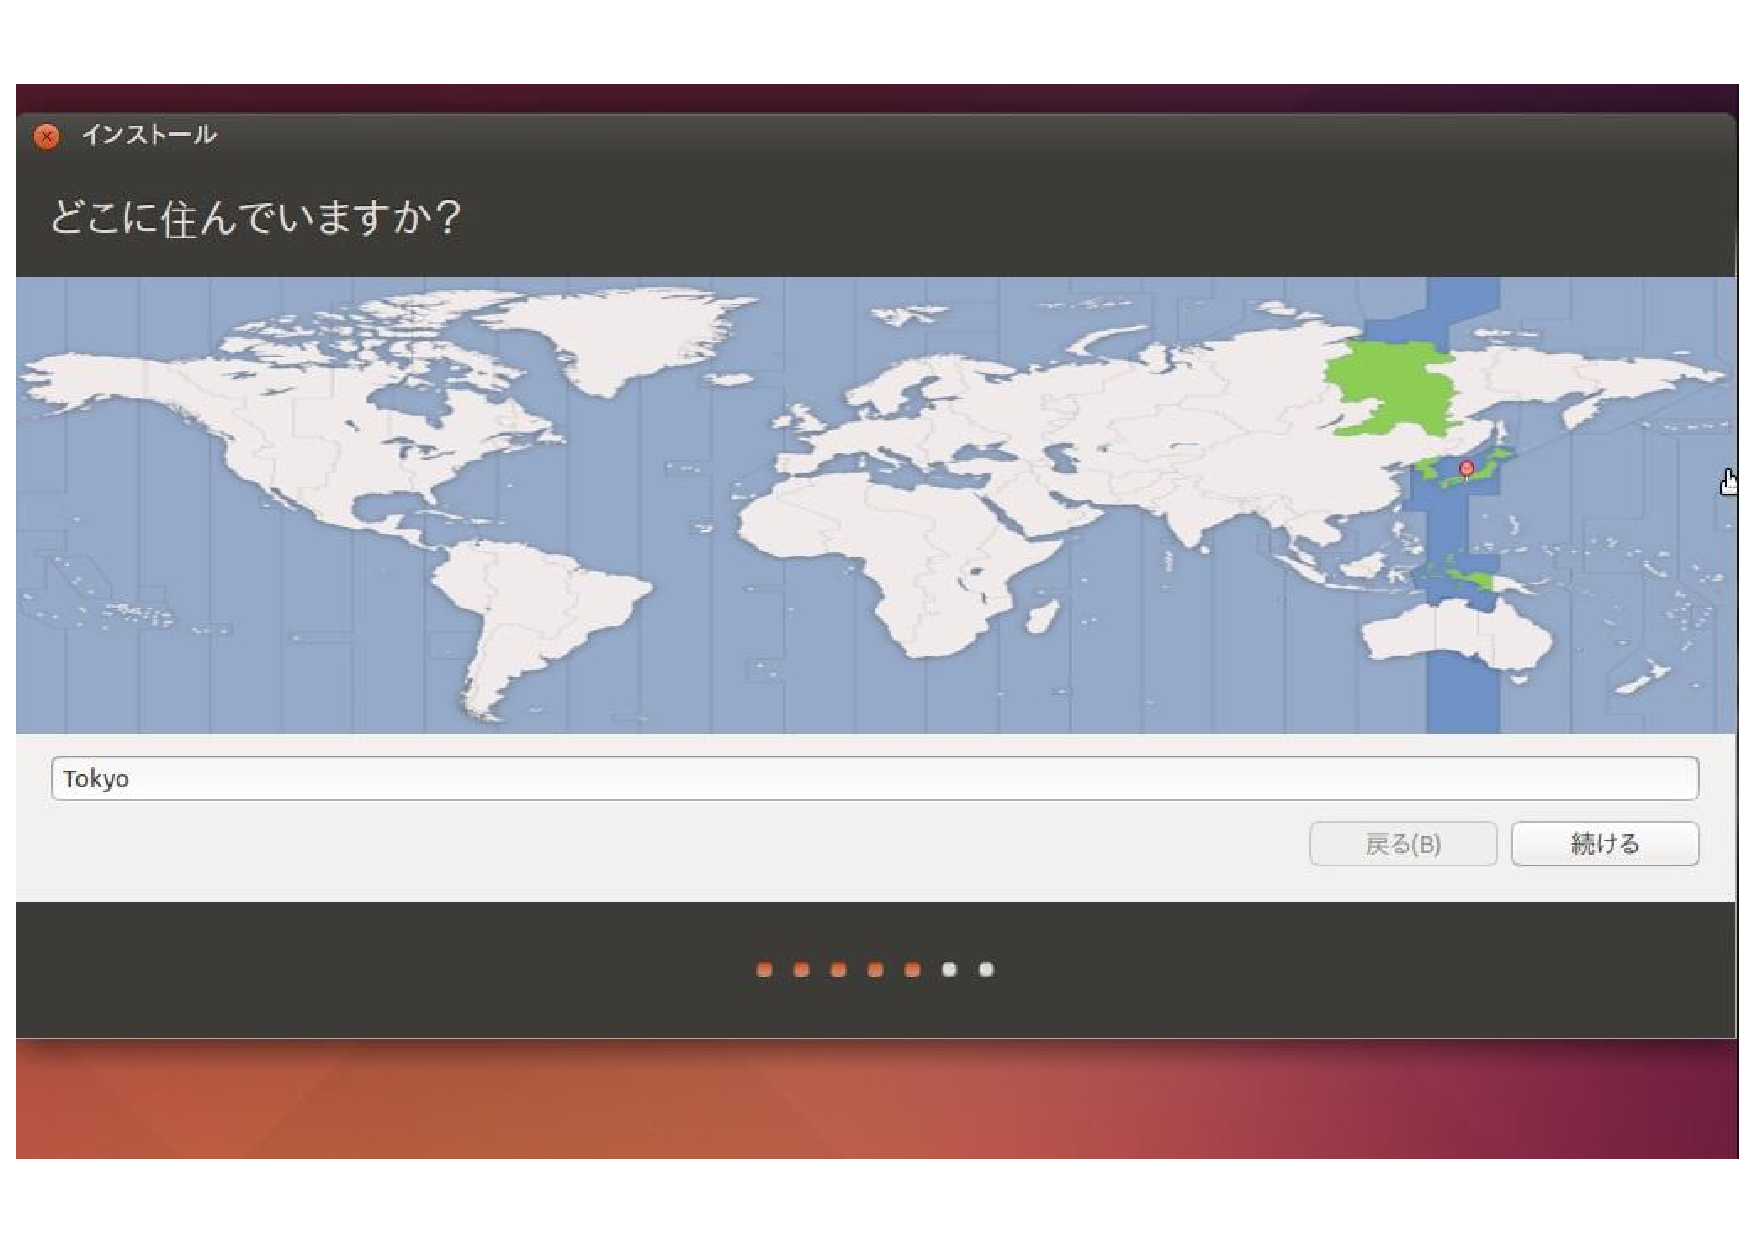
\includegraphics[width=13cm]{figure11.pdf}
\caption{Ubuntuの導入5}\label{sannp}
\end{figure}

\begin{figure}[H]
\centering
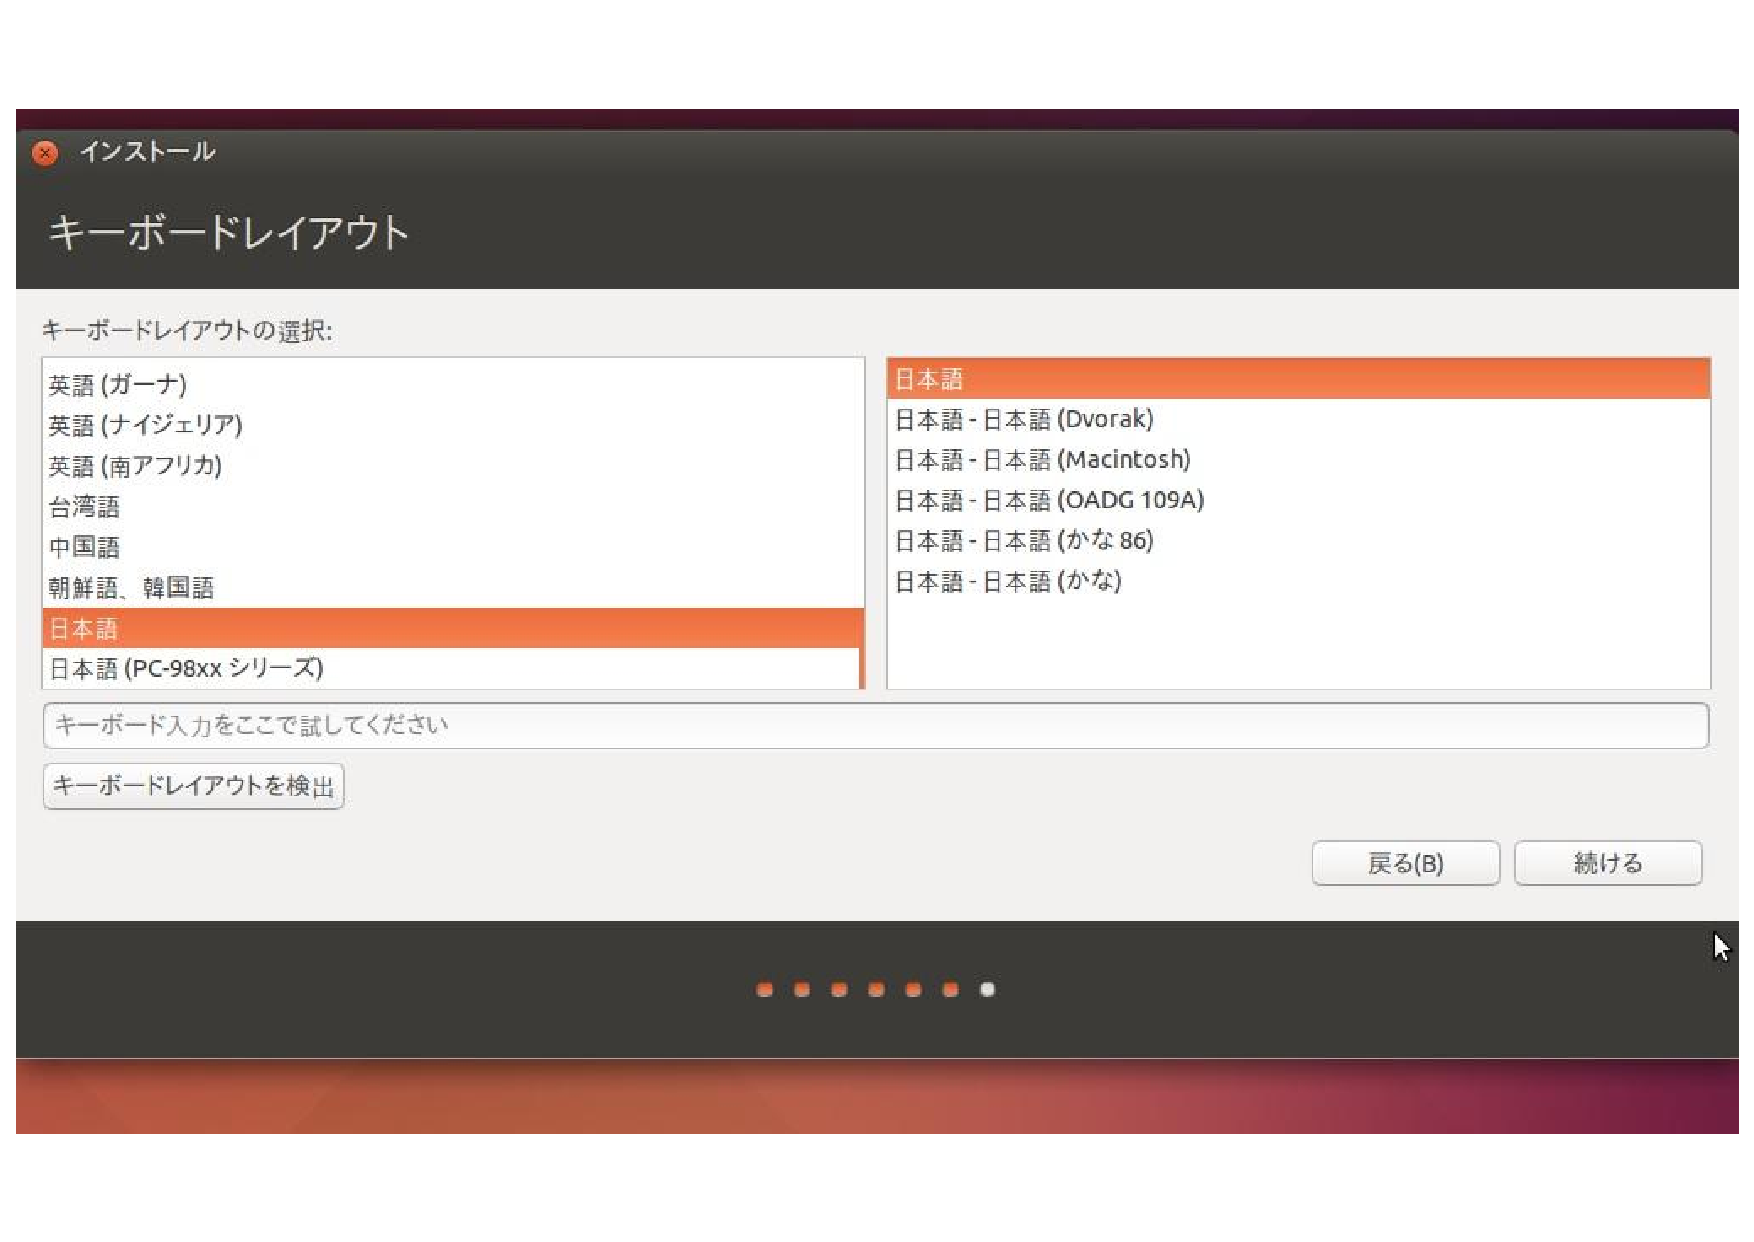
\includegraphics[width=13cm]{figure12.pdf}
\caption{Ubuntuの導入6}\label{sannp}
\end{figure}

進めるとユーザーの設定とパスワードの設定を行う.ここで使用するパスワードはroot化をする際などでも使用するため,忘れないように保存をしておく.続けるを選択するとインストールが始まる.

\begin{figure}[H]
\centering
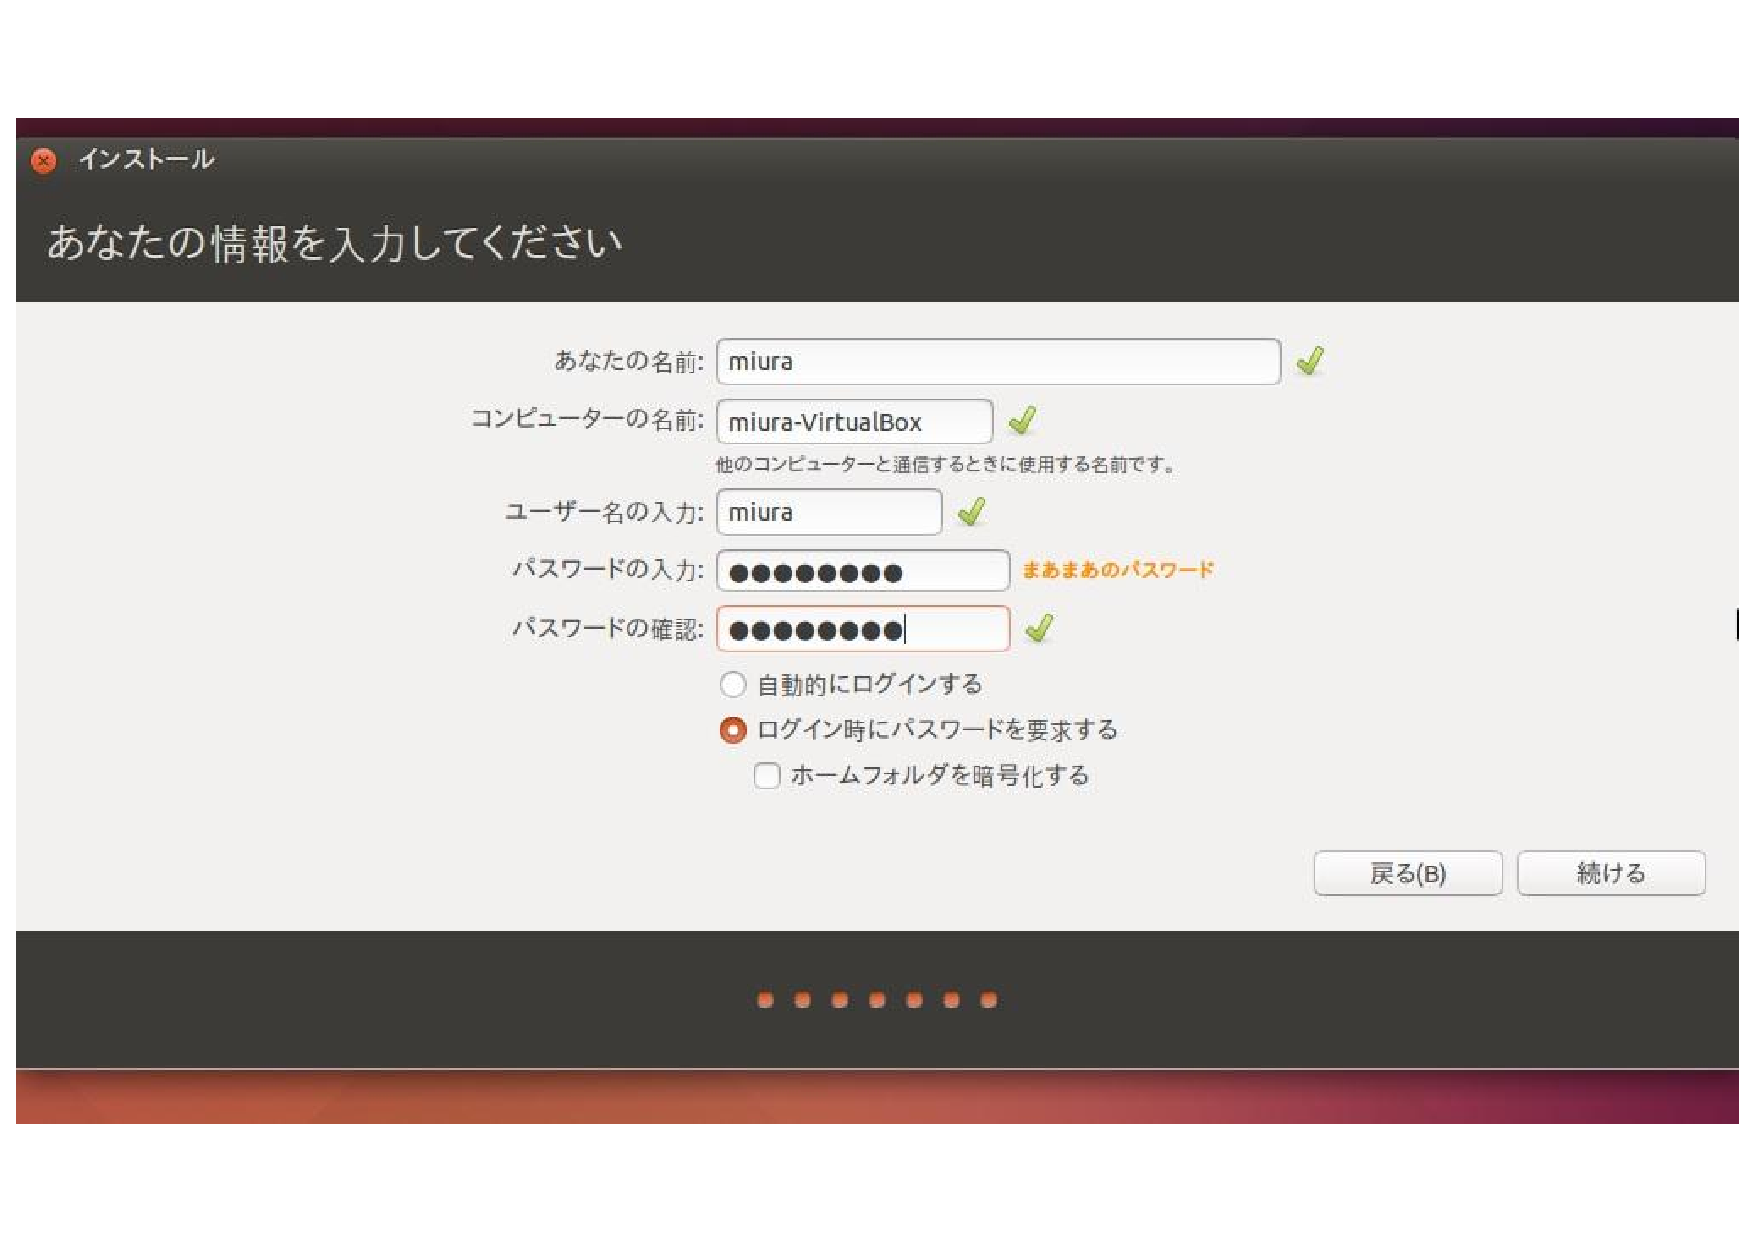
\includegraphics[width=13cm]{figure13.pdf}
\caption{Ubuntuの導入7}\label{sannp}
\end{figure}

\begin{figure}[H]
\centering
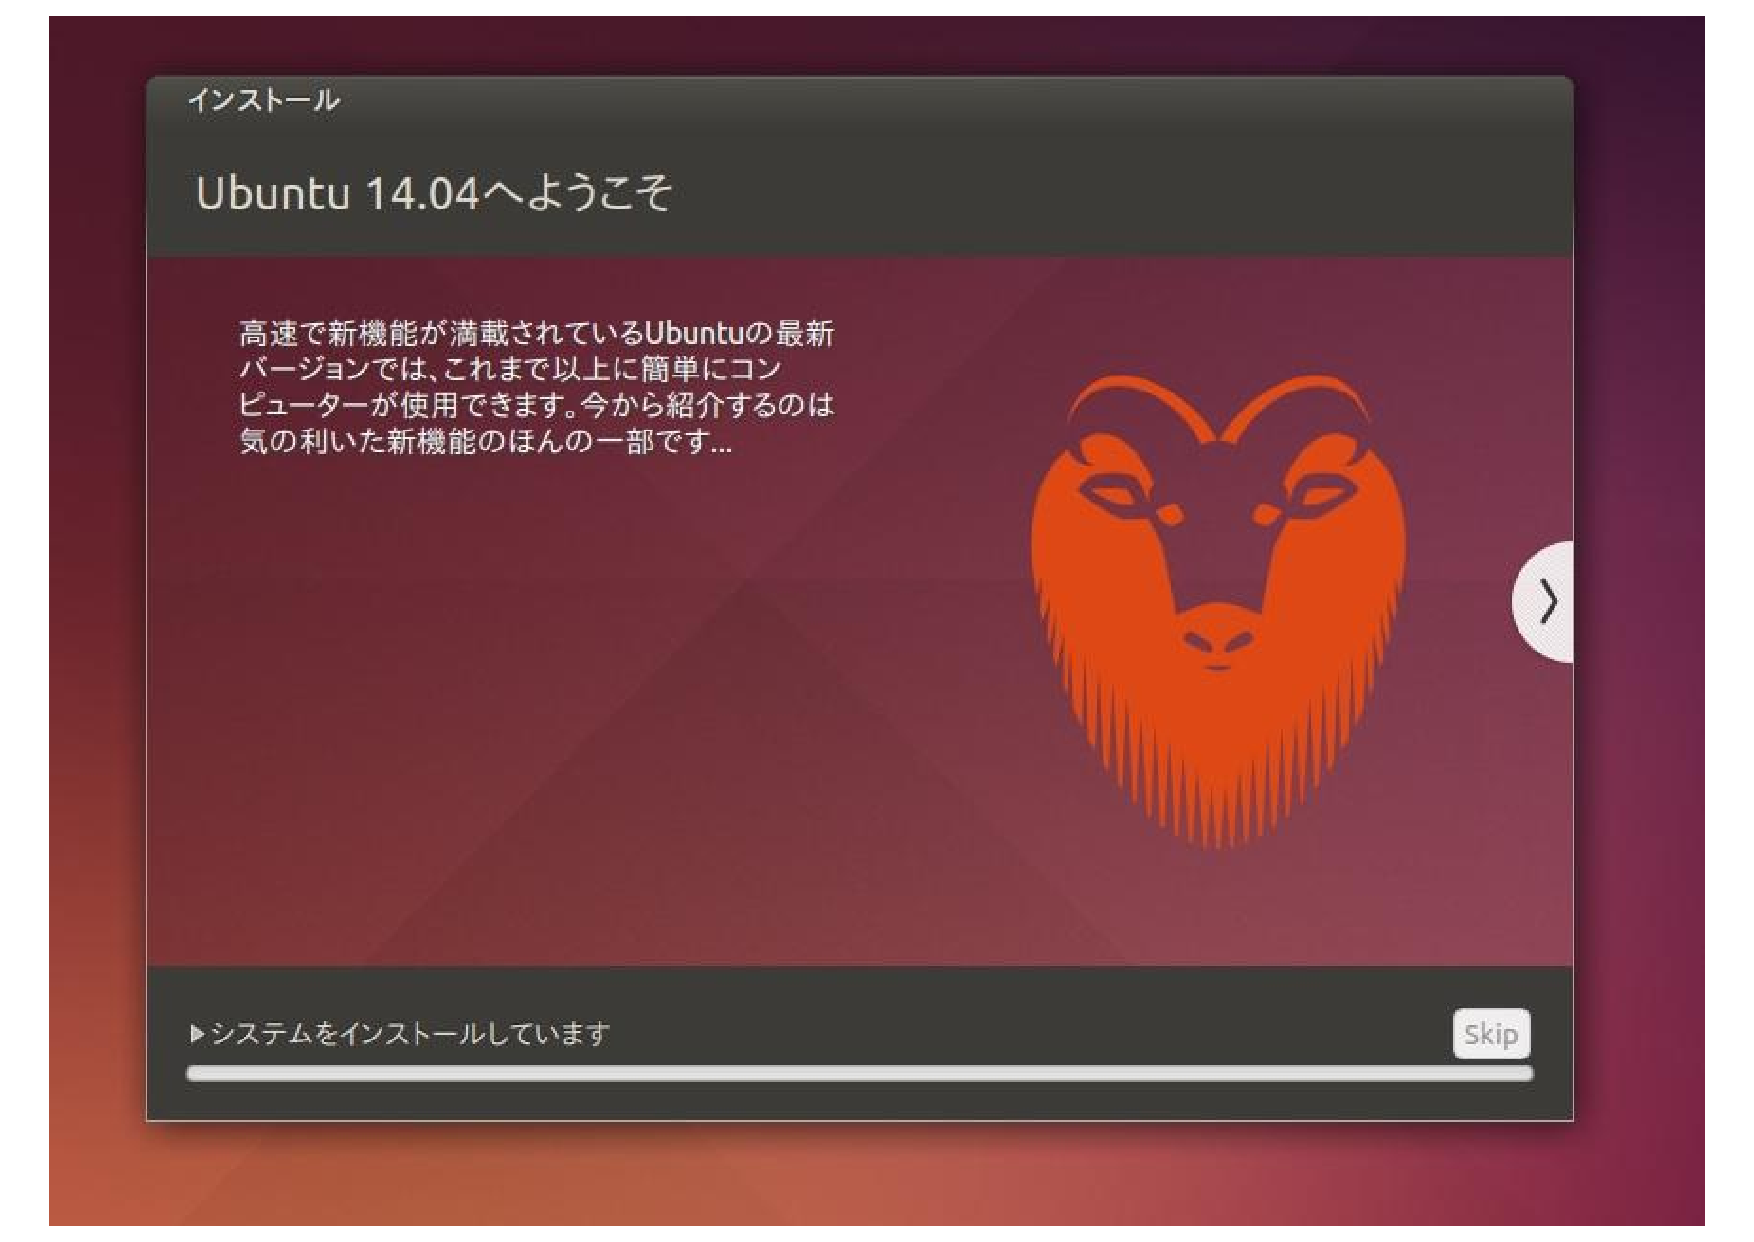
\includegraphics[width=13cm]{figure14.pdf}
\caption{Ubuntuの導入8}\label{sannp}
\end{figure}

インストール完了が表示されたら再起動を行う.

\begin{figure}[H]
\centering
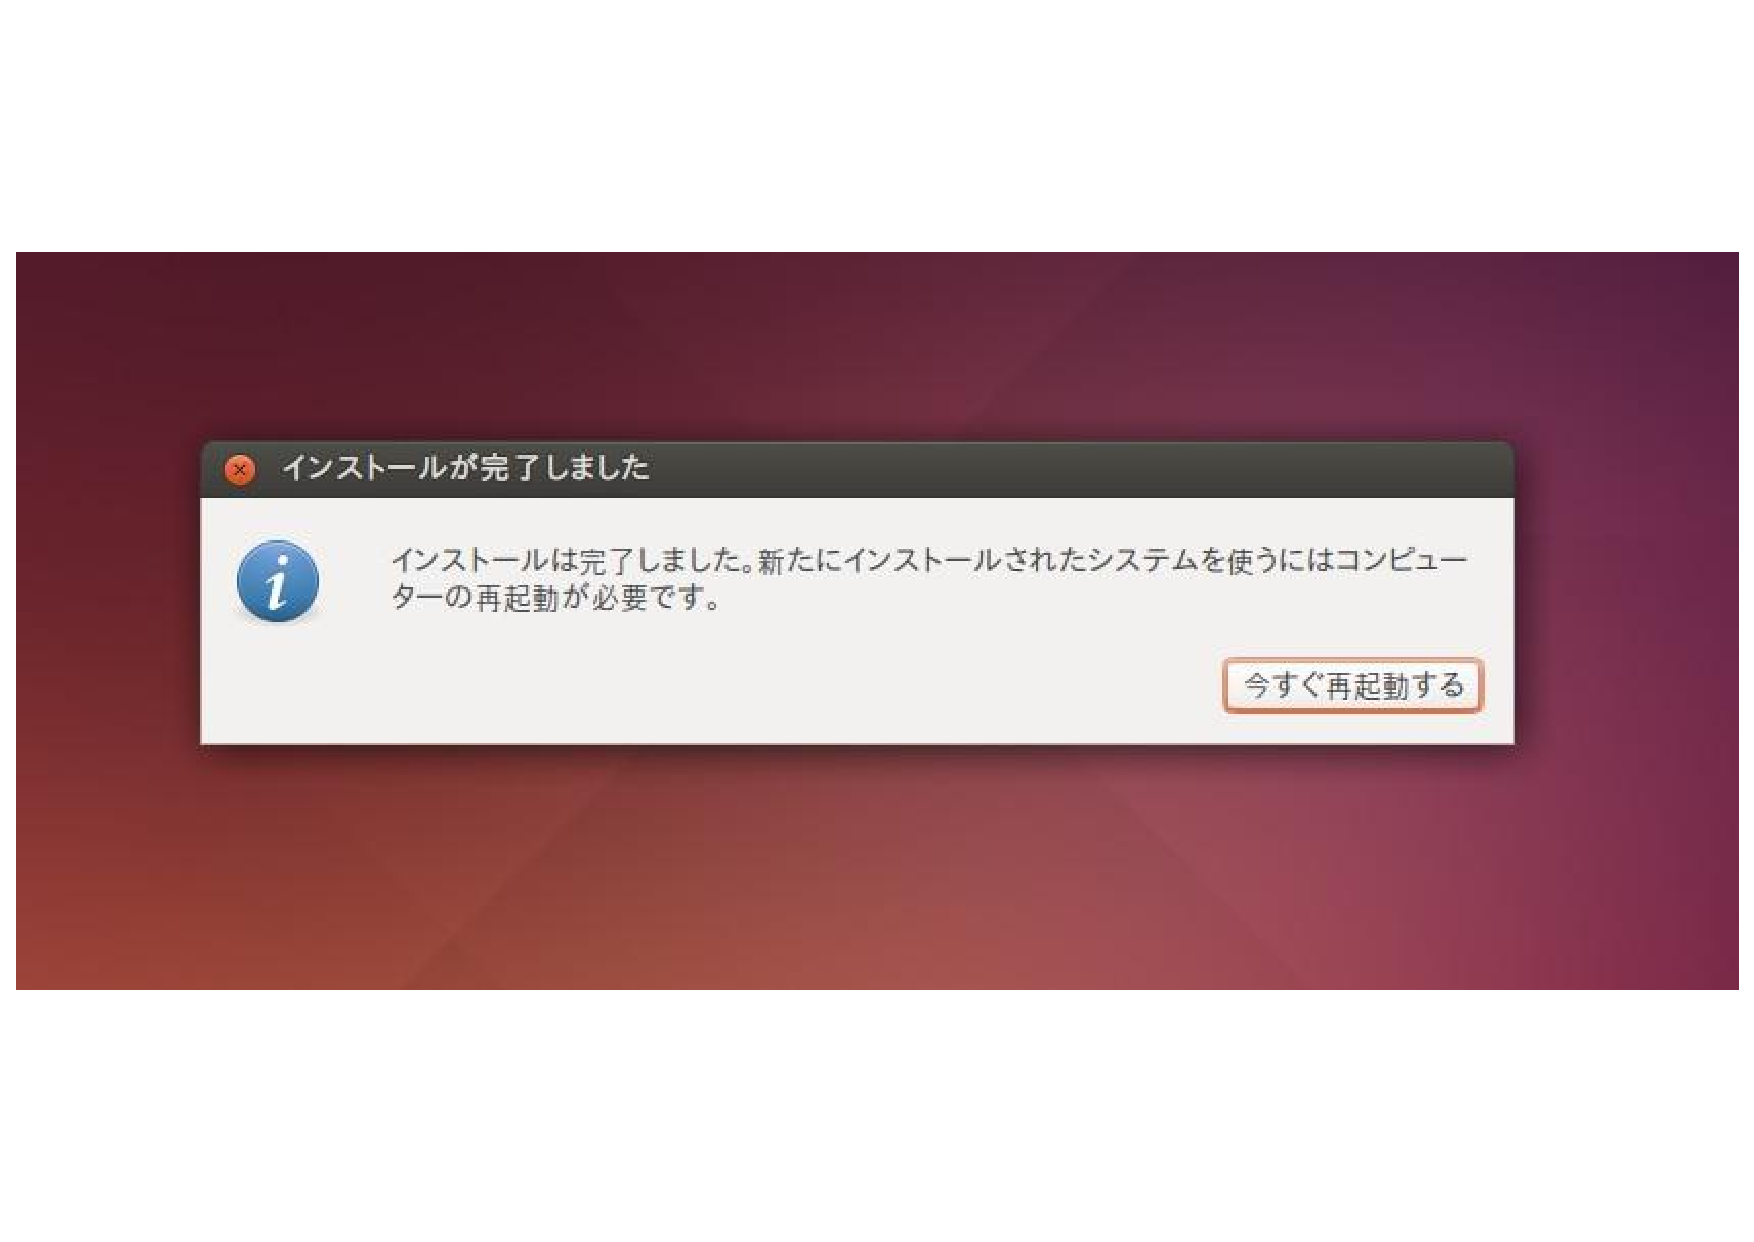
\includegraphics[width=13cm]{figure15.pdf}
\caption{Ubuntuの導入9}\label{sannp}
\end{figure}

\section{クローラーの導入}
Ubuntu上でクローラーを運用する手順を解説する.
\begin{figure}[h]
\centering
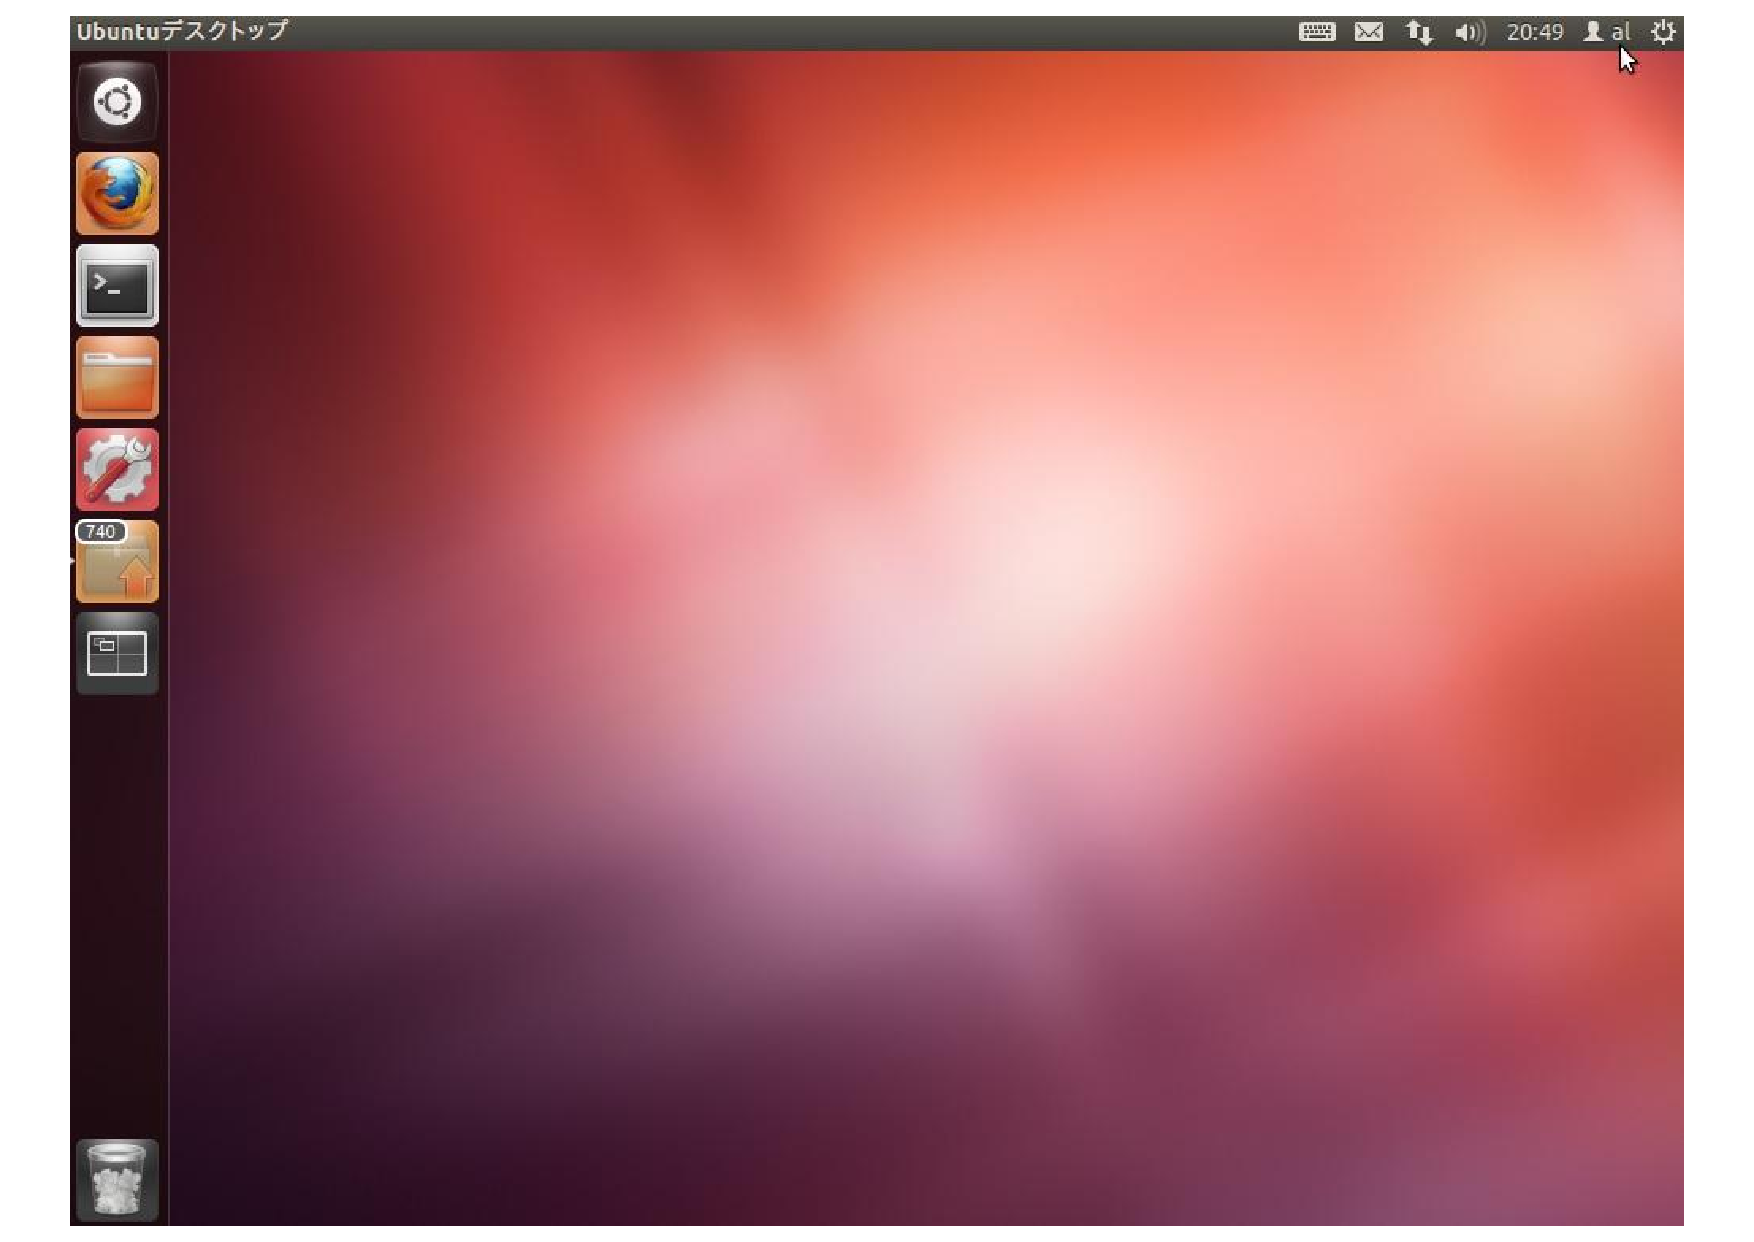
\includegraphics[width=13cm]{figure3.pdf}
\caption{クローラーの導入}\label{sannp}
\end{figure}

ホーム上にクローラーのプログラムを今回はシェルで書く,説明のためにファイルの名前をhozon.shとする.

\begin{figure}[H]
\centering
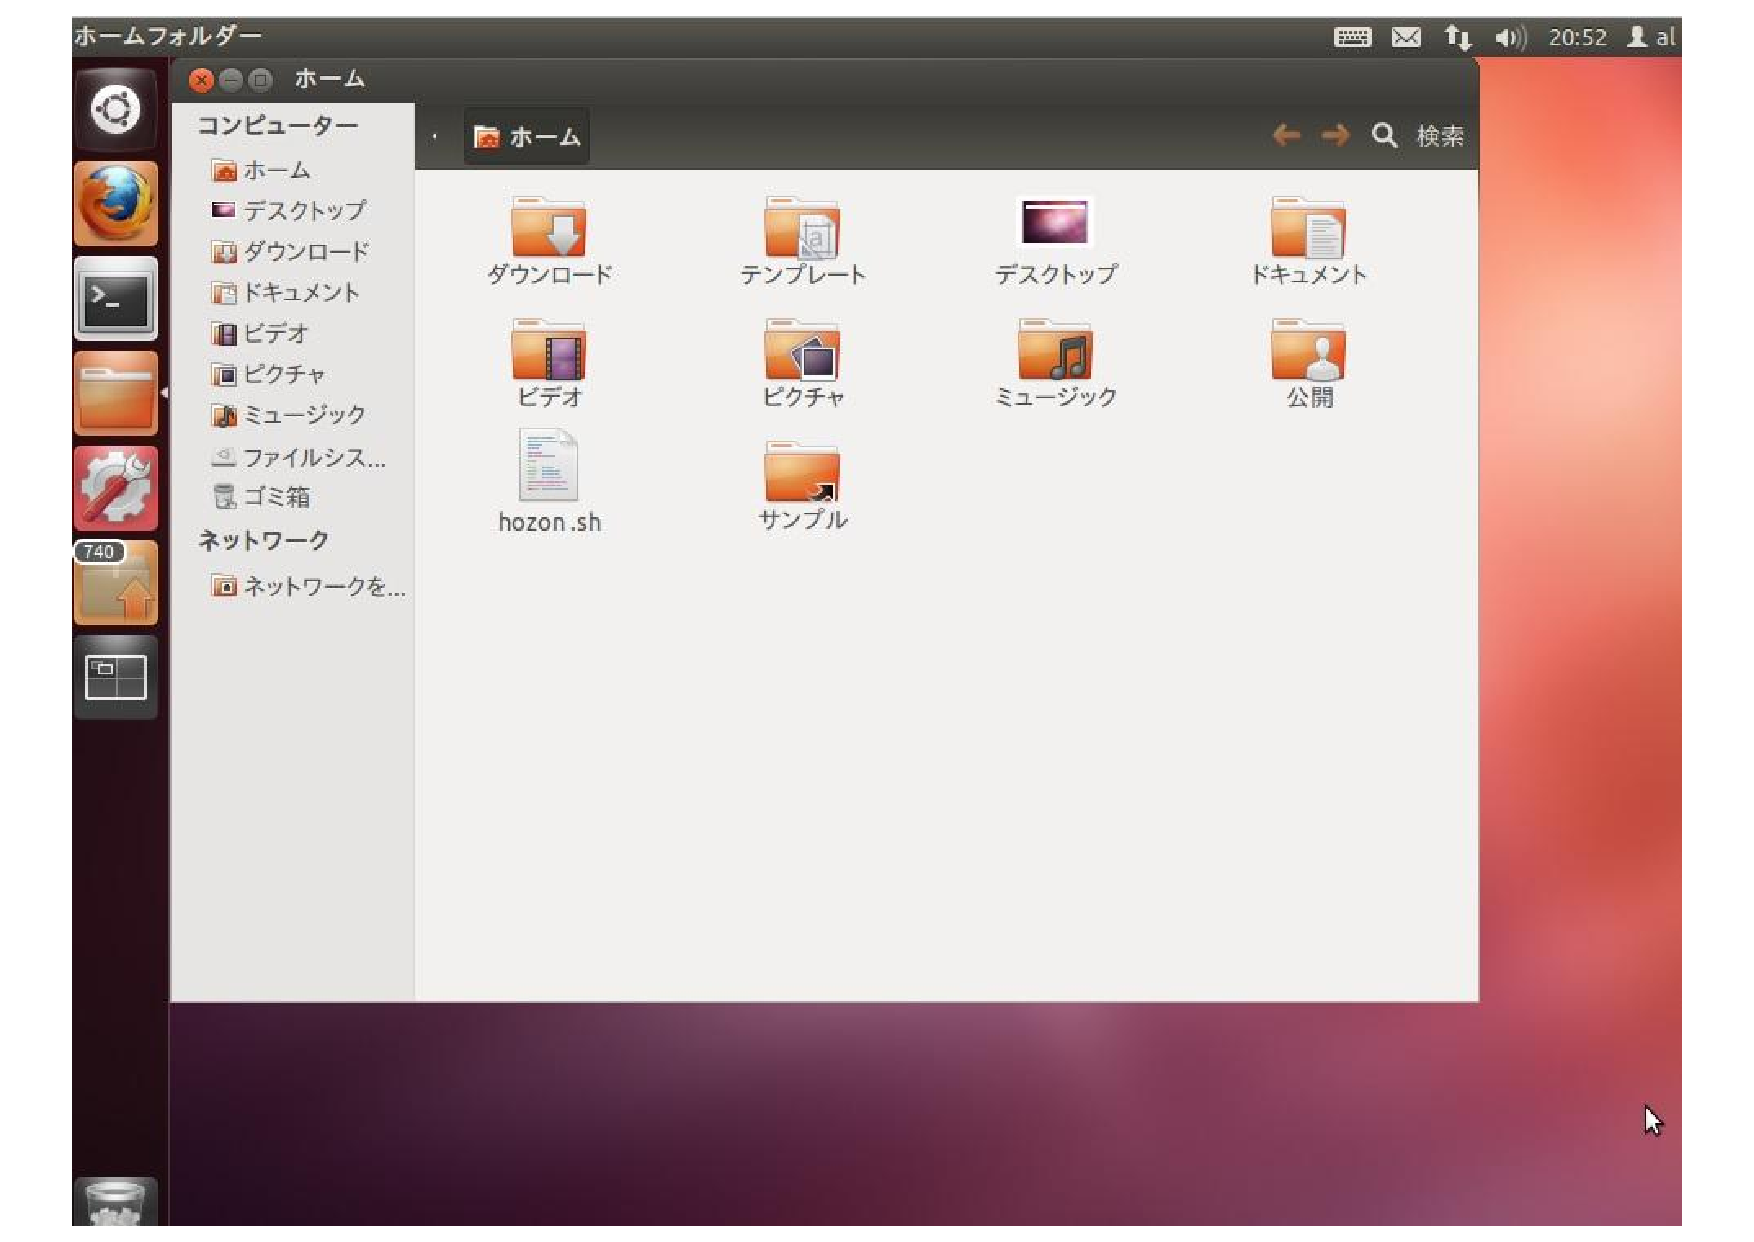
\includegraphics[width=13cm]{figure4.pdf}
\caption{クローラーの導入2}\label{sannp}
\end{figure}

hozon.shの内容は以下のとおりである.

\begin{figure}[H]
\centering
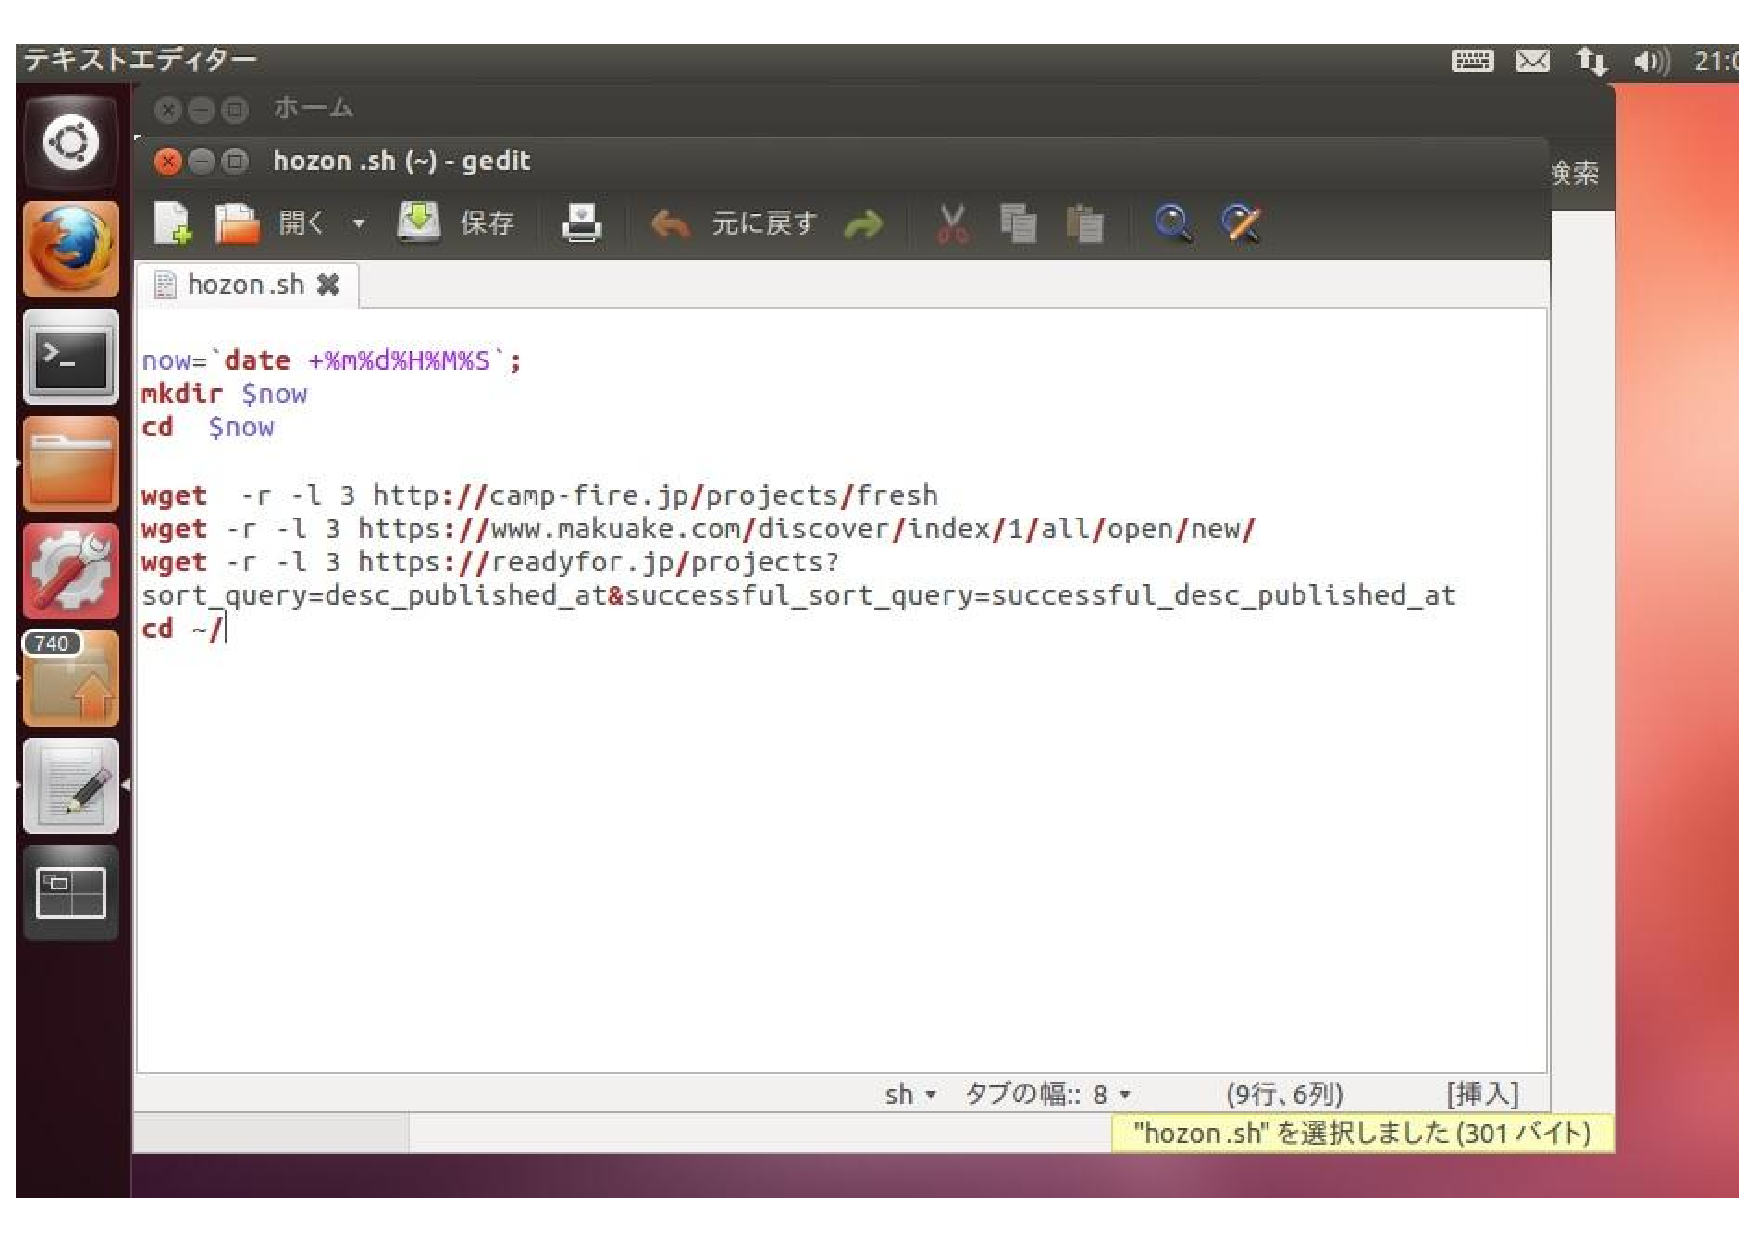
\includegraphics[width=13cm]{figure5.pdf}
\caption{クローラーの導入3}\label{sannp}
\end{figure}

毎日,同時刻にデータを収集する際に,同じフォルダで保存し続けるのを避けるため,Linuxコマンドのdata,cd,mkdirを組み合わせてプログラムが動き出した現在時刻をフォルダ名に設定するようにしてある.wgetを利用し,各サイトごとに順番にスタート設定したURLから再帰的にファイルを入手するように設定してある.以下に今回使用したコマンドの解説を記す.

\begin{table}[H]
  \begin{center}
    \caption{[date]日付,時刻を表示,設定する}
    \begin{tabular}{|l|c|} \hline
      文字 & 解説  \\ \hline
\%H & 時 (00~23) \\
\%I & 時 (01~12) \\
\%k & 時 ( 0~23) \\
\%l & 時 ( 1~12) \\
\%M & 分 (00~59) \\
\%p & AM あるいは PM のロケール(国や地域に合わせた文字列) \\
\%r & 12時間形式の時刻 (HH:mm:ss [AP]M) \\
\%s & 1970-01-01 00:00:00 UTC からの秒数 \\
\%S & 秒 (00~61) \\
\%T & 24時間形式の時刻 (HH:mm:ss) \\
\%a & ロケールによる省略形の曜日の名前 (Sun~Sat) \\
\%A & ロケールによる完全に表記した曜日の名前(Sunday~Saturday) \\
\%b & ロケールによる省略形の月の名前 (Jan~Dec) \\
\%B & ロケールによる完全に表記した月の名前(January~December) \\
\%c & ロケールによる日付と時刻 (Sat Nov 04 12:02:33 EST 1989) \\
\%d & 日(月内通算日数) (01~31) \\
\%D & 日付 (MM/DD/YY) \\
\%j & 年内通算日数 (001~366) \\
\%m & 月 (01~12) \\
\%w & 週のうちの曜日(0~6)で0が日曜日に対応 \\
\%x & ロケールによる日付の表現 (MM/DD/YY) \\
\%y & 西暦の下2けた (00~99) \\
\%Y & 年 (1970~) \\ \hline
 \end{tabular}
  \end{center}
\end{table}


\begin{table}[H]
  \begin{center}
    \caption{[cd] ディレクトリを移動する}
    \begin{tabular}{|l|c|} \hline
      文字 & 解説  \\ \hline
   / & ルート・ディレクトリ \\
    . & 現在のディレクトリ \\
   … & 親ディレクトリ \\
  \~/ & ホーム・ディレクトリ \\ \hline
    \end{tabular}
  \end{center}
\end{table}

\begin{table}[H]
  \begin{center}
    \caption{[mkdir] ディレクトリを作成する}
    \begin{tabular}{|l|c|} \hline
      文字 & 解説  \\ \hline
   -m & ディレクトリのモードを設定する \\
    -p & 指定したディレクトリをサブディレクトリごと作成する. \\
   -v & ディレクトリを作成する毎にメッセージを出力する \\
   --help & mkdirコマンドの使用法を表示する \\
--version	& バージョン情報を標準出力に表示する \\
directory & 作成するディレクトリ名を指定する \\ \hline
    \end{tabular}
  \end{center}
\end{table}

\begin{figure}[H]
\centering
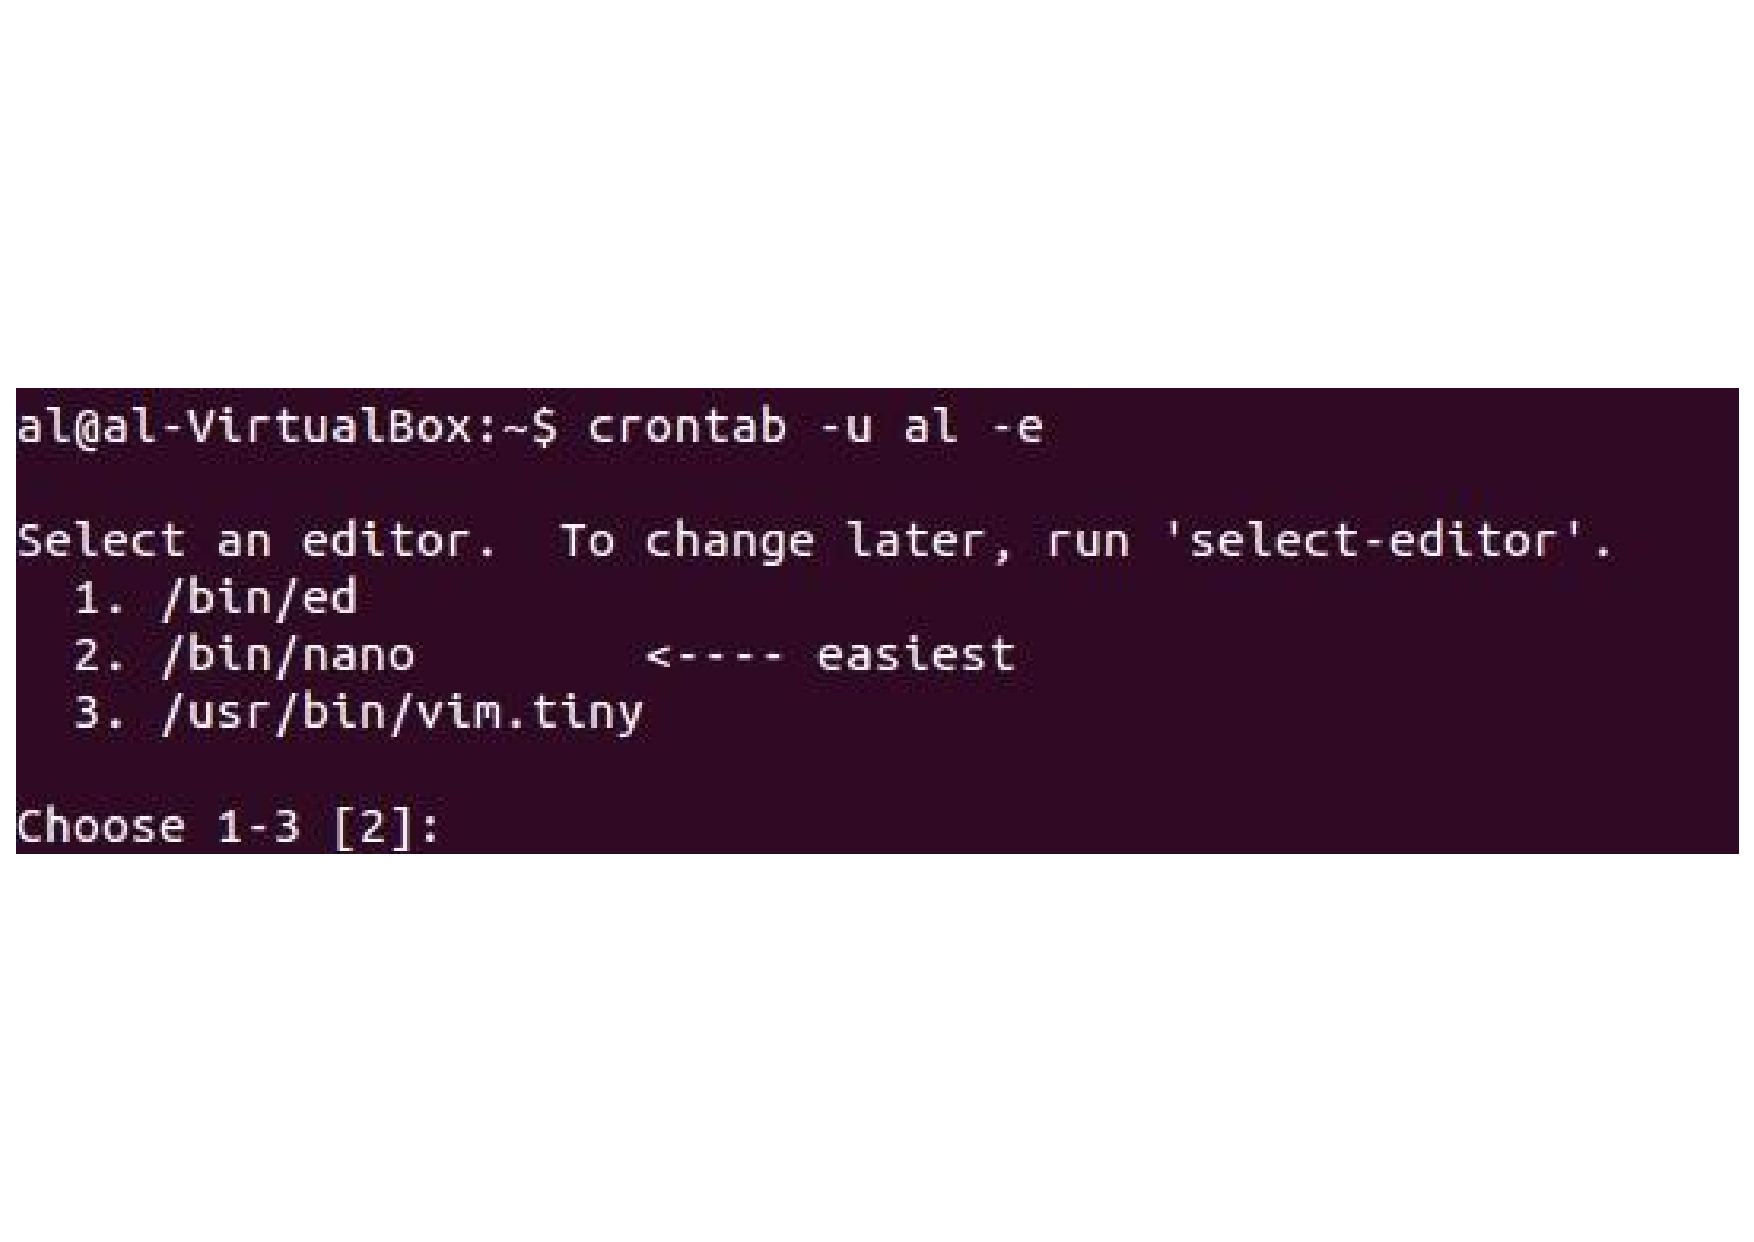
\includegraphics[width=13cm]{figure6.pdf}
\caption{クローラーの導入4}\label{sannp}
\end{figure}

ホーム上にあるシェルを毎日,同じ時間に自動で動かすために,端末からcrontabを利用して時間が来たらシェルを呼び出し,プログラムをスタートするように設定する.

\begin{itemize}
 \item 端末を起動し,crontab -u ユーザー名 -e と入力をし,Enterを押す.
 \item 表示された3つの選択肢の中から好きなエディターを選ぶことができる.今回は2を選択する.
 \item 2を入力しEnterを押すと下記の画面が表示される
\end{itemize}

\begin{figure}[H]
\centering
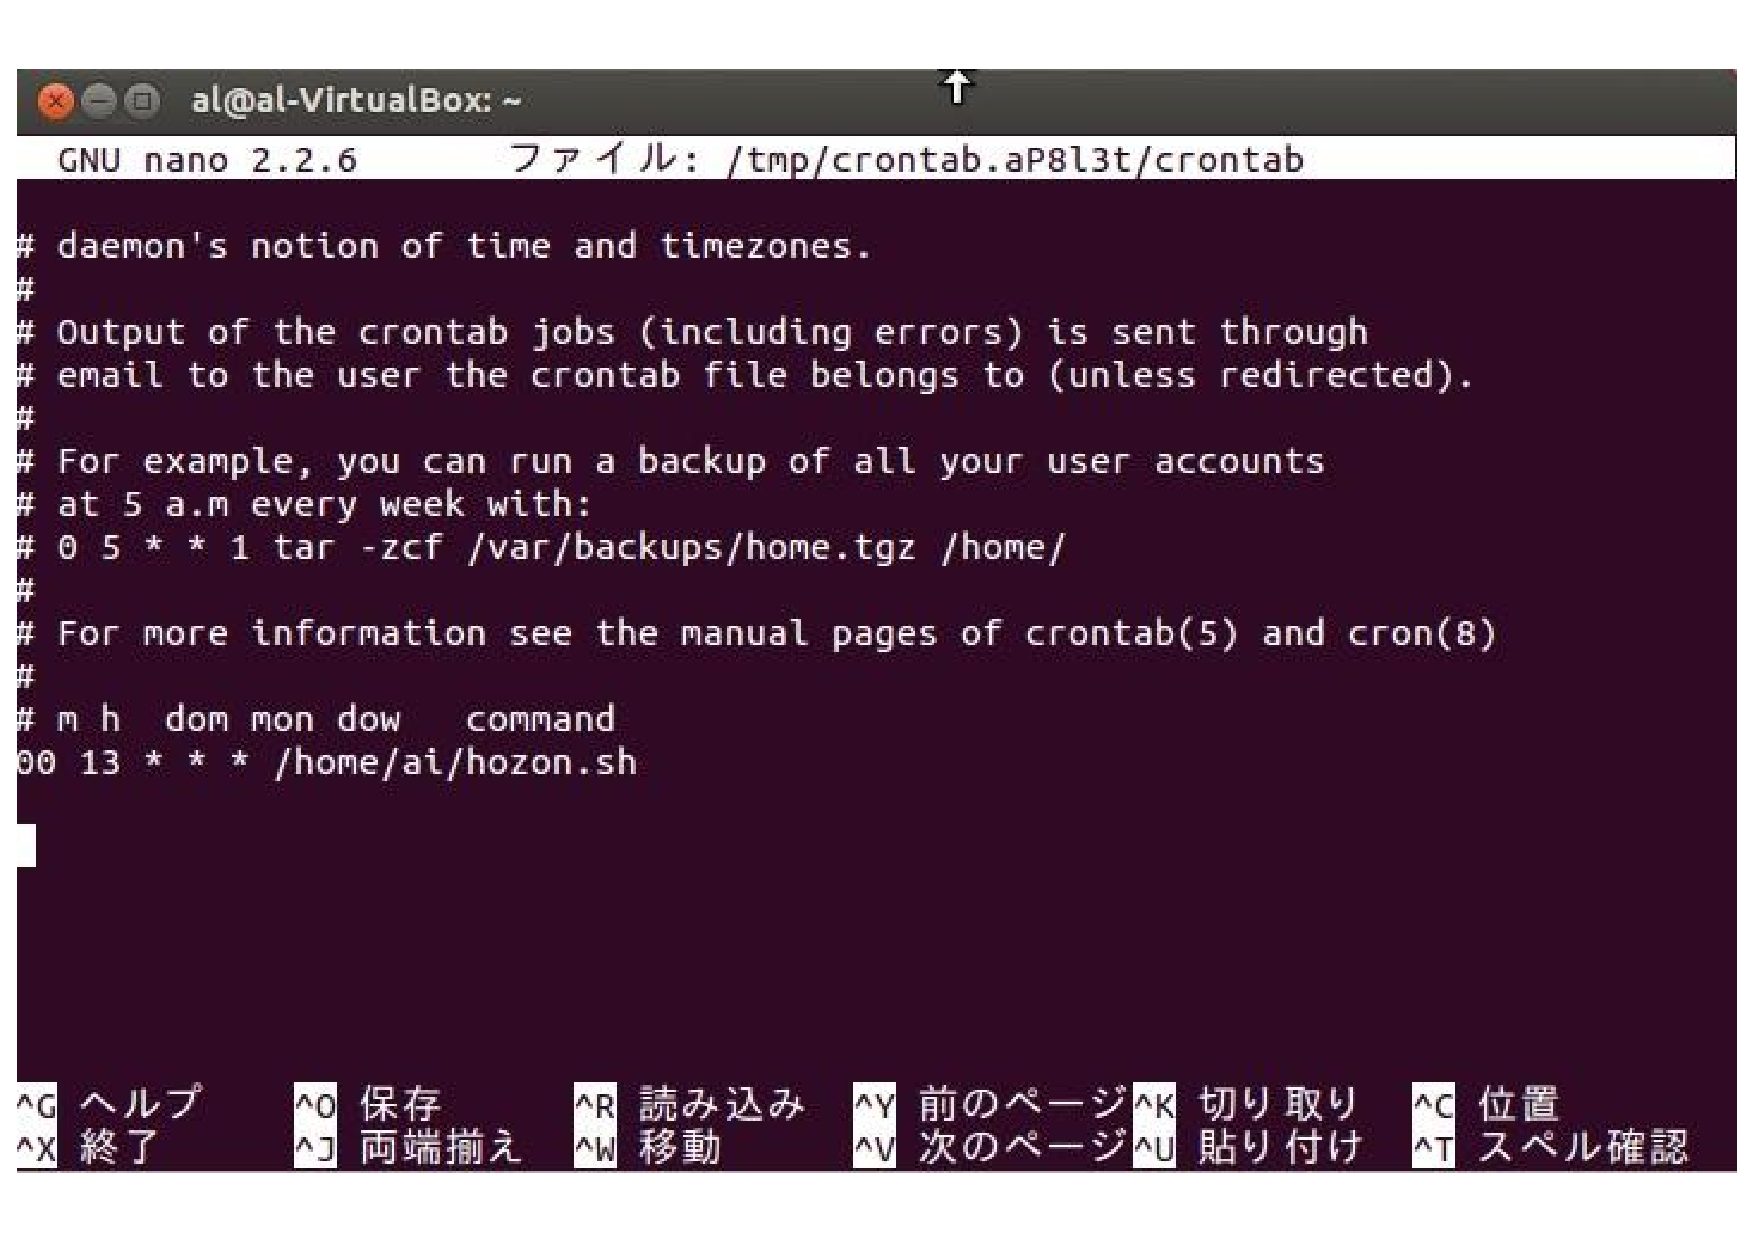
\includegraphics[width=13cm]{figure7.pdf}
\caption{クローラーの導入5}\label{sannp}
\end{figure}

エディターでプログラムを行う時刻とプログラムを指定する.文法は以下のとおりである.

分 時 日 月 曜日 コマンド

\begin{table}[H]
  \begin{center}
    \caption{記述方法}
    \begin{tabular}{|l|c|} \hline
      文法 & 解説  \\ \hline
分 & 分を「0~59」で指定する。ワイルドカード(*)を記述すると毎分となる。 \\
時 & 時間を「0~23」で指定する。ワイルドカード(*)を記述すると毎時となる。 \\
日 & 日を「1~31」で指定する。ワイルドカード(*)を記述すると毎日となる。 \\
月 & 月を「1~12」もしくは「jan~dec」で指定する。ワイルドカード(*)を記述すると毎月となる。 \\
曜日 & 曜日を「0~7」(0,7は日曜日)もしくは「sun~sat」で指定する。ワイルドカード(*)を記述すると毎日となる。 \\
コマンド & 実行したいコマンドやシェルを記述します。 \\ \hline
    \end{tabular}
  \end{center}
\end{table}

今回のクローラーの稼働設定を例としてあげると,

00 13 * * * /home/al/hozon.sh   

毎日13:00に/home/alにあるhozon.shを実行するいう命令になる.

\chapter{本論}

\section{本章の構成}
本章では,研究方法と実際に行った研究手順について記載する.

\section{研究手順}
本研究では以下の手順で研究を行った.
\begin{enumerate}
 \item クローラーで定期的に対象のサイトを監視,情報を収集する.
 \item 集めた情報を元にデータマイニングを用いて判別分析を行う.
 \item 得られた結果を考察し,要因を探し出す.
\end{enumerate}

\chapter{クローラーの運用について}

\section{対象サイトについて}
本研究では日本でクラウドファンディングを行うことを想定し,日本でもっとも市場が大きい「購入型」のプロジェクトを対象に情報を収集することとする.
また利用者数が多い,Makuake(\url{https://www.makuake.com/})とREADYFOR(\url{https://readyfor.jp/})の2サイトに掲載されているものを対象とし,無差別に掲載されているプロジェクトを収集する.
\begin{figure}[H]
\centering
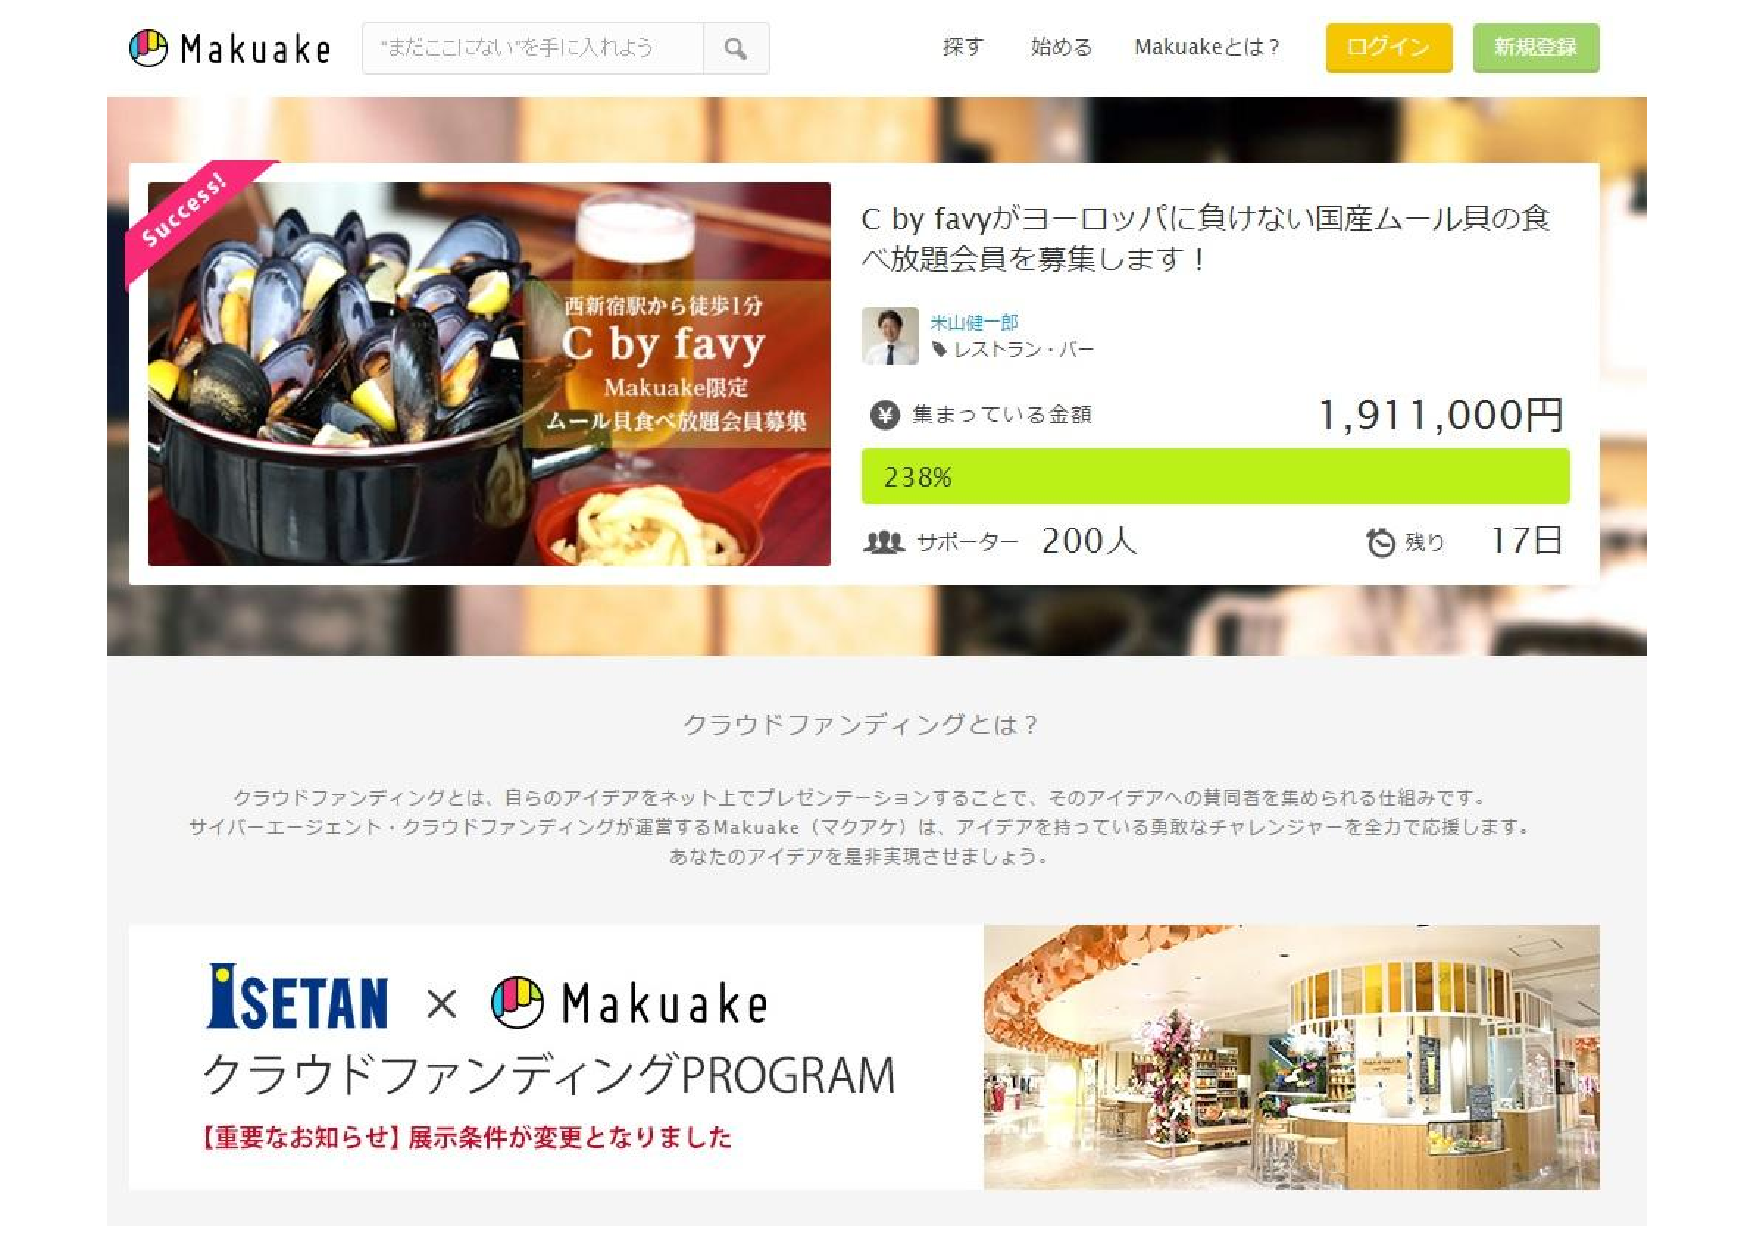
\includegraphics[width=10cm]{figure16.pdf}
\caption{Makuake}\label{sannp}
\end{figure}

\begin{figure}[H]
\centering
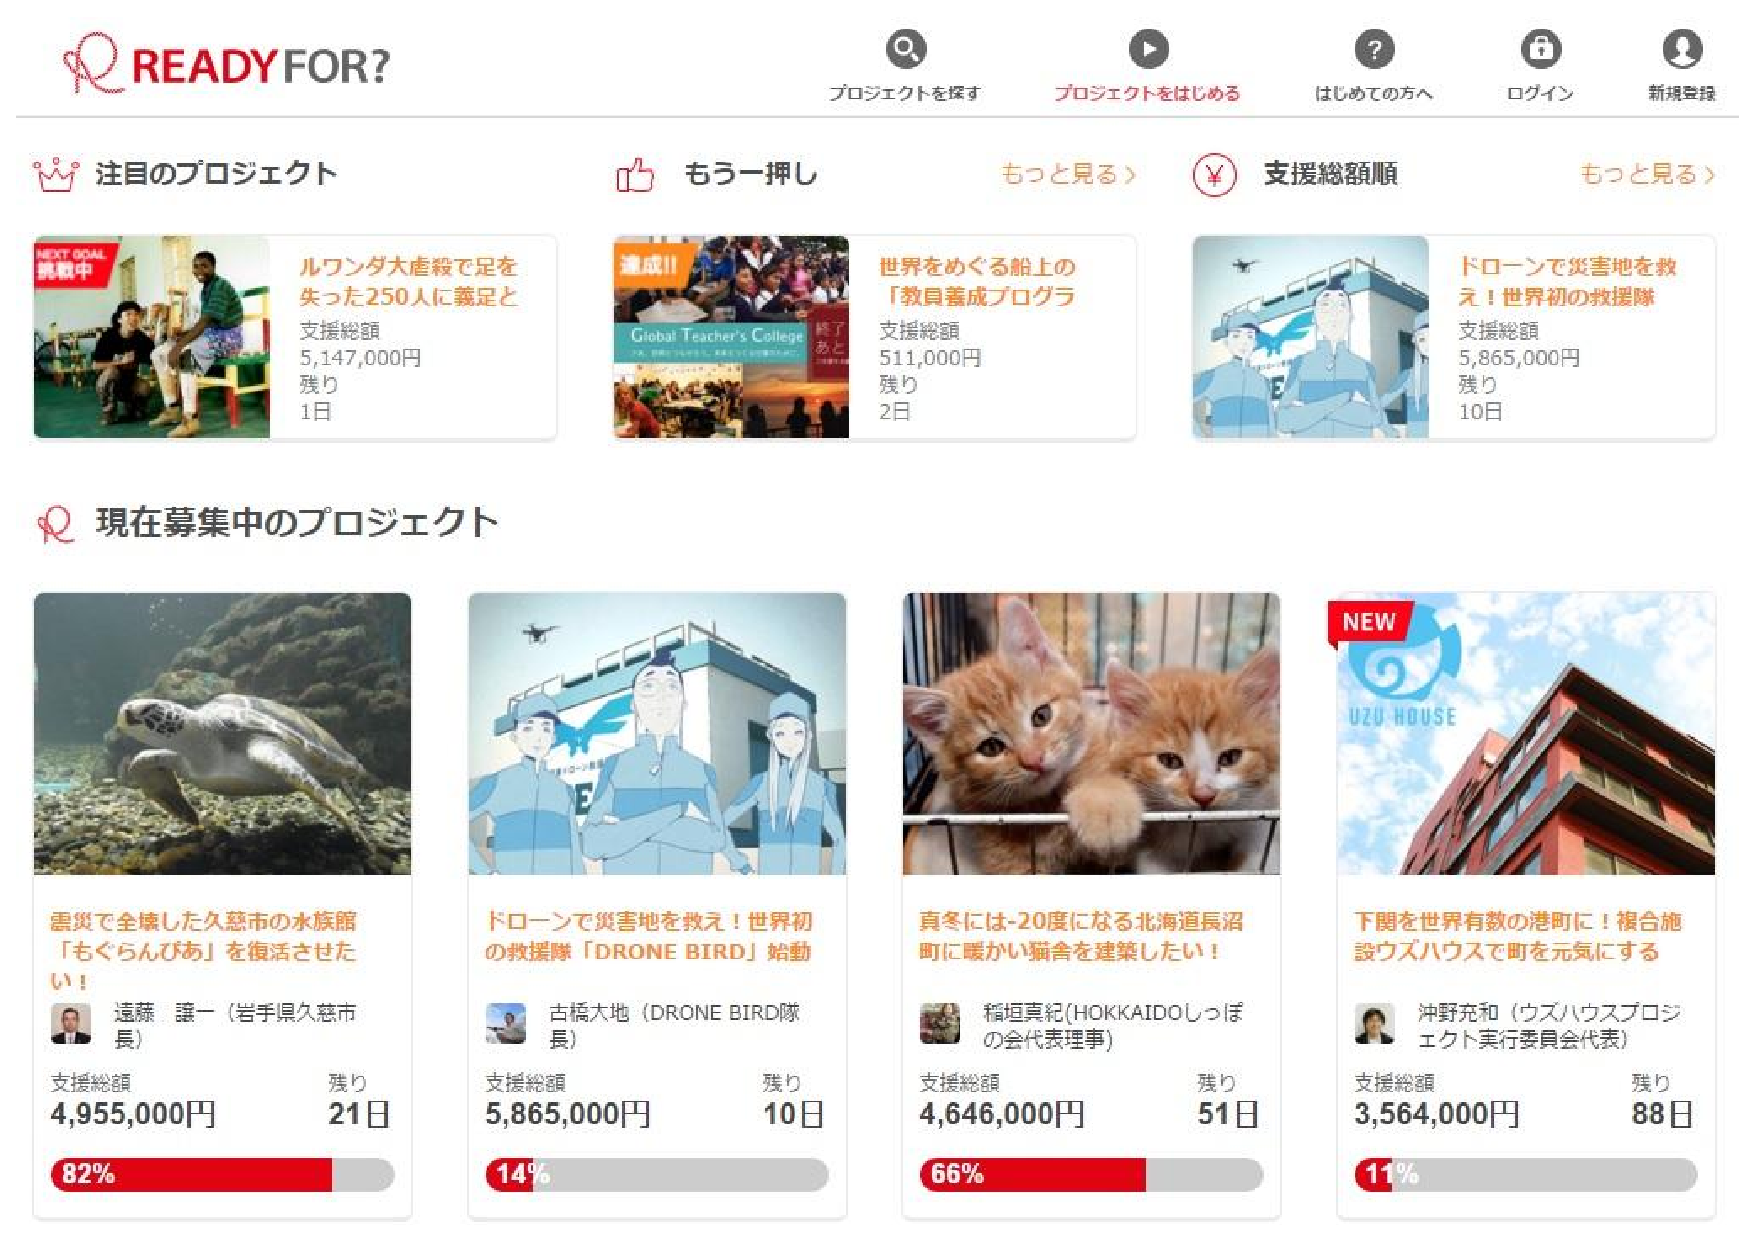
\includegraphics[width=10cm]{figure17.pdf}
\caption{READYFOR}\label{sannp}
\end{figure}



\section{ディレクトリ構造について}

序論でに記載したクローラーを使用し,実際にデータを集めると下記のフォルダが自動的に生成される.
今回は毎日毎時13時からクローラーを動かしデータを収集した.

\begin{figure}[H]
\centering
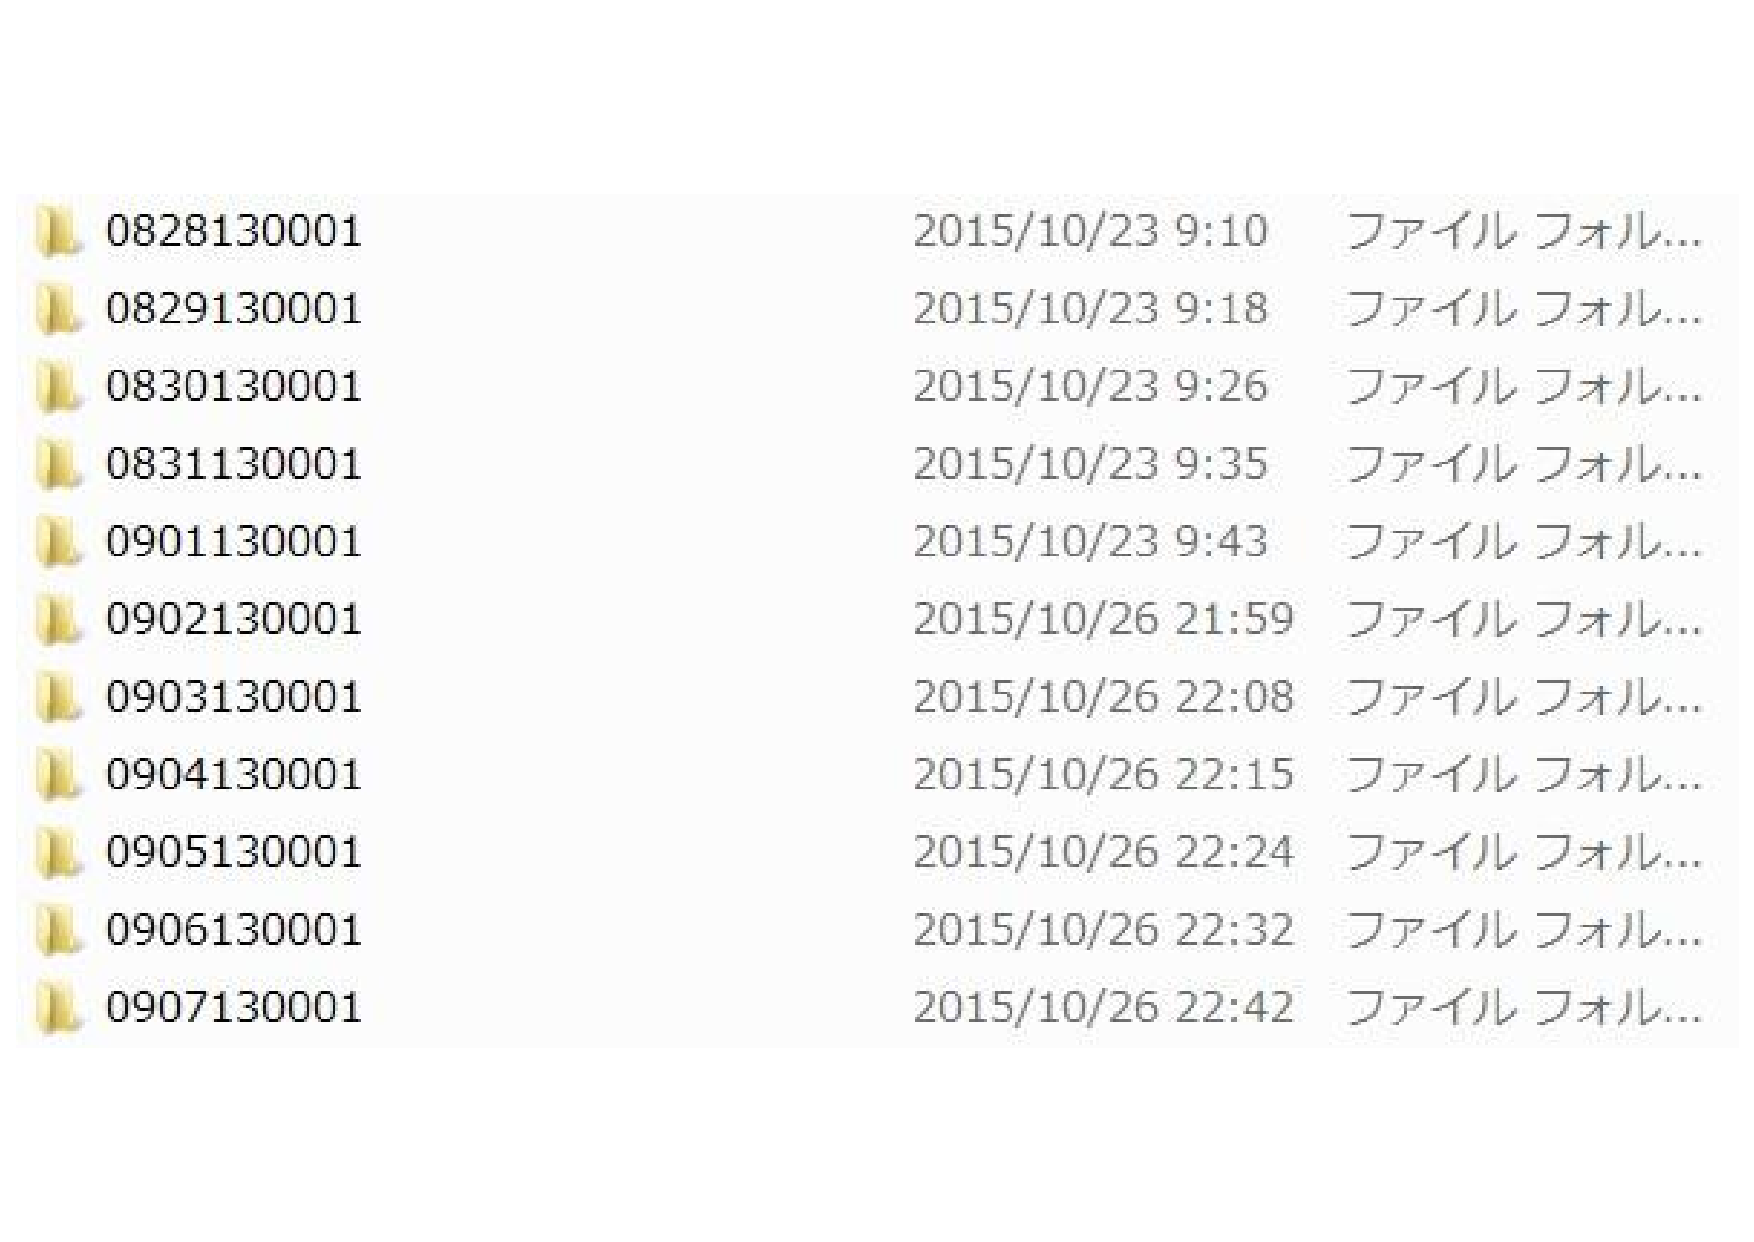
\includegraphics[width=13cm]{figure29.pdf}
\caption{実際のディレクトリ1}\label{sannp}
\end{figure}

フォルダ名は実行した月日時分秒となっており,0828130001であれば8月28日13時00分01秒に実行した分のデータとなる.
\begin{figure}[H]
\centering
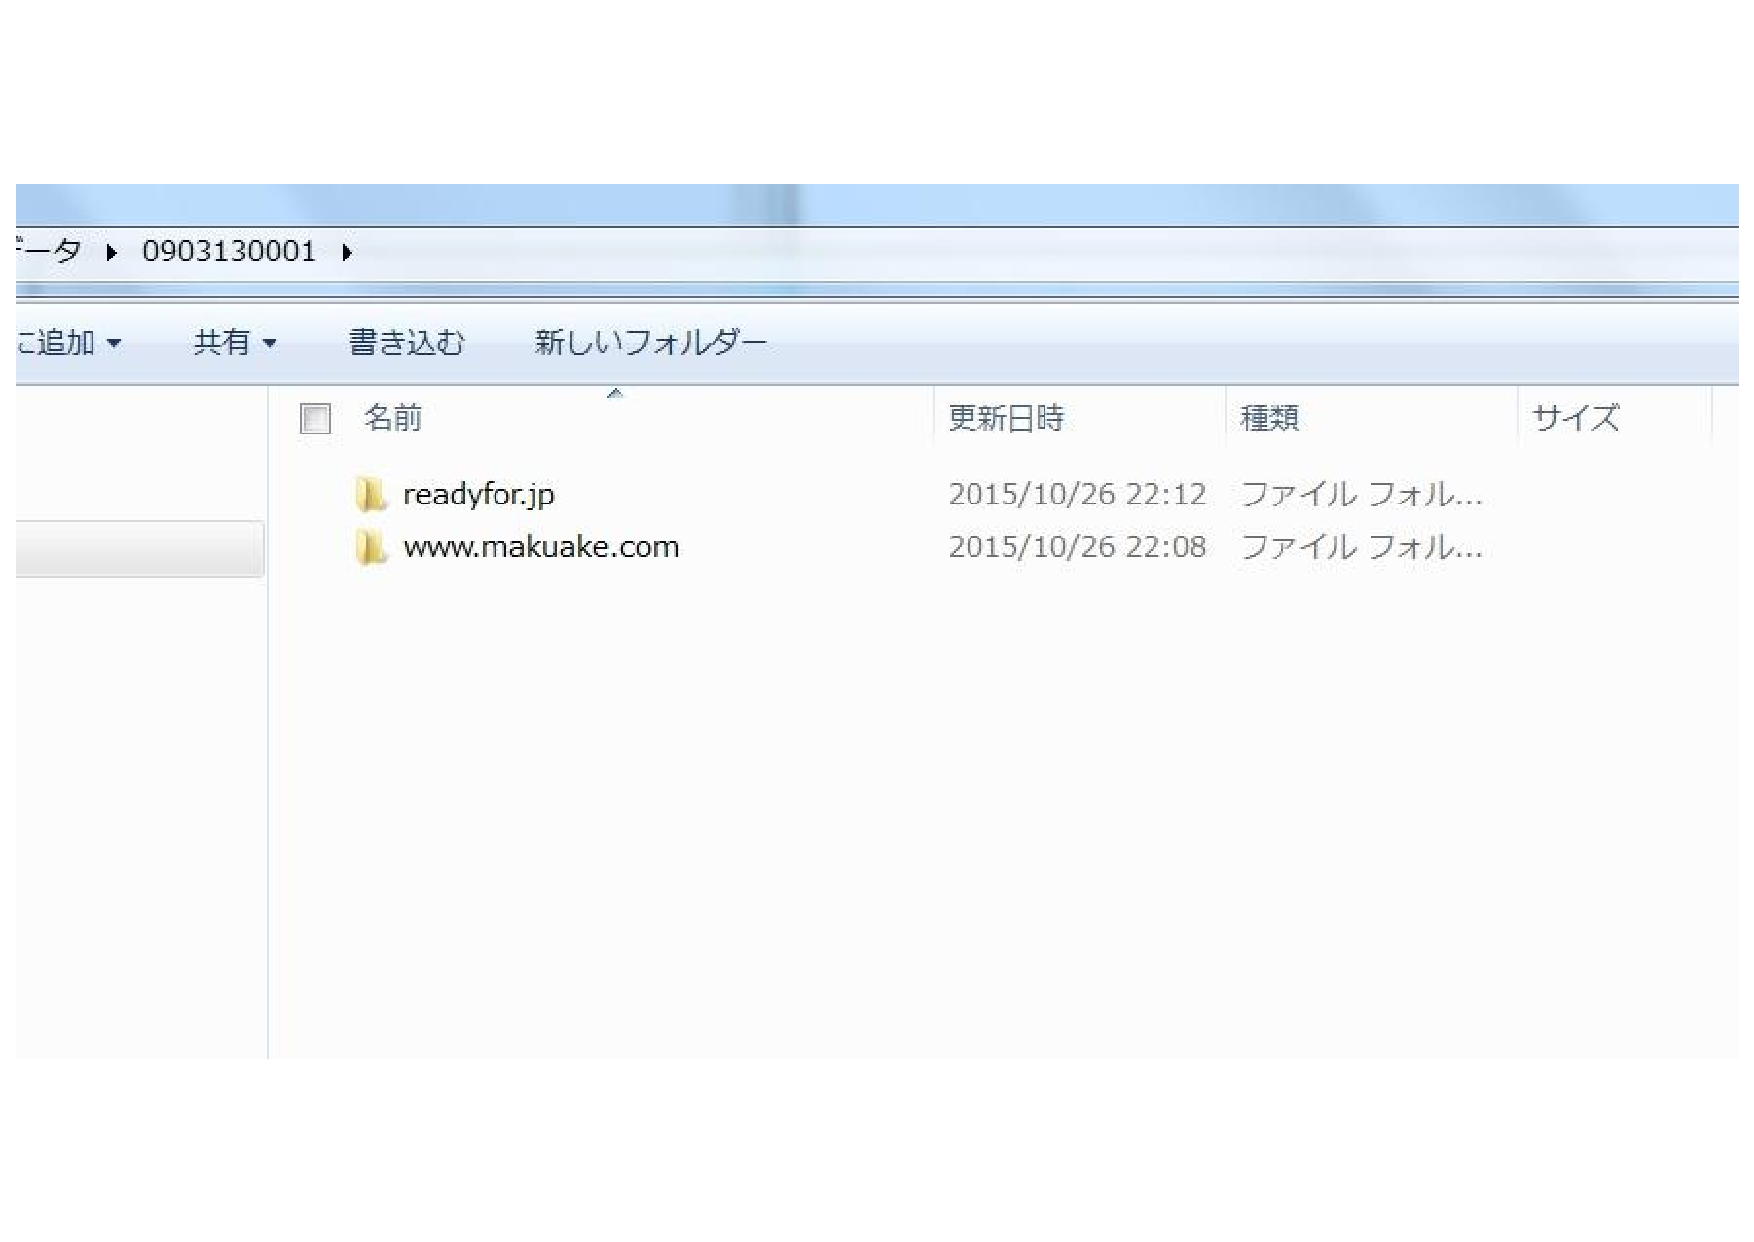
\includegraphics[width=13cm]{figure33.pdf}
\caption{実際のディレクトリ2}\label{sannp}
\end{figure}

フォルダ内のデータは,初めにサイト毎にフォルダが分かれており,二つのサイトが混ざることはない.初めにREADYFORのディレクトリから説明をしていく.

\begin{figure}[H]
\centering
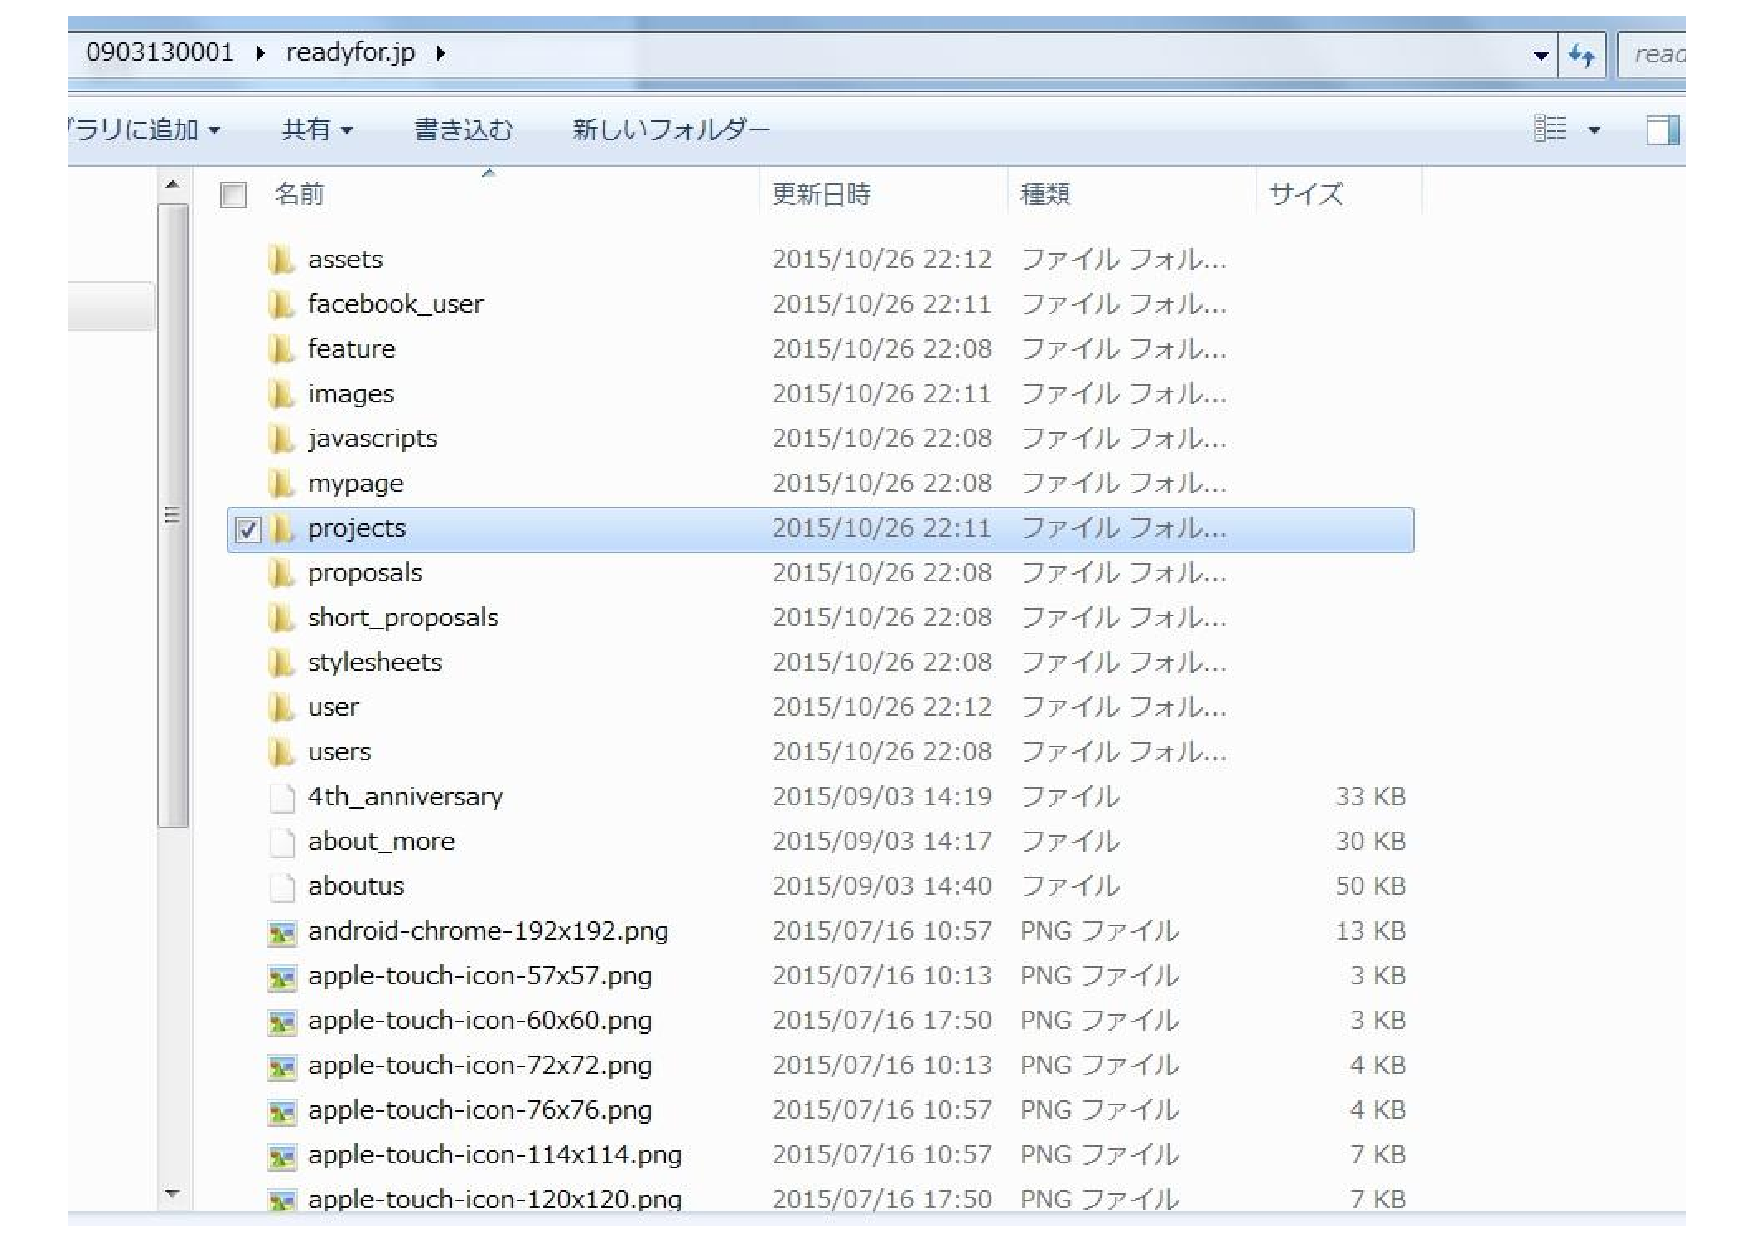
\includegraphics[width=13cm]{figure30.pdf}
\caption{READYFORのディレクトリ1}\label{sannp}
\end{figure}

\begin{figure}[H]
\centering
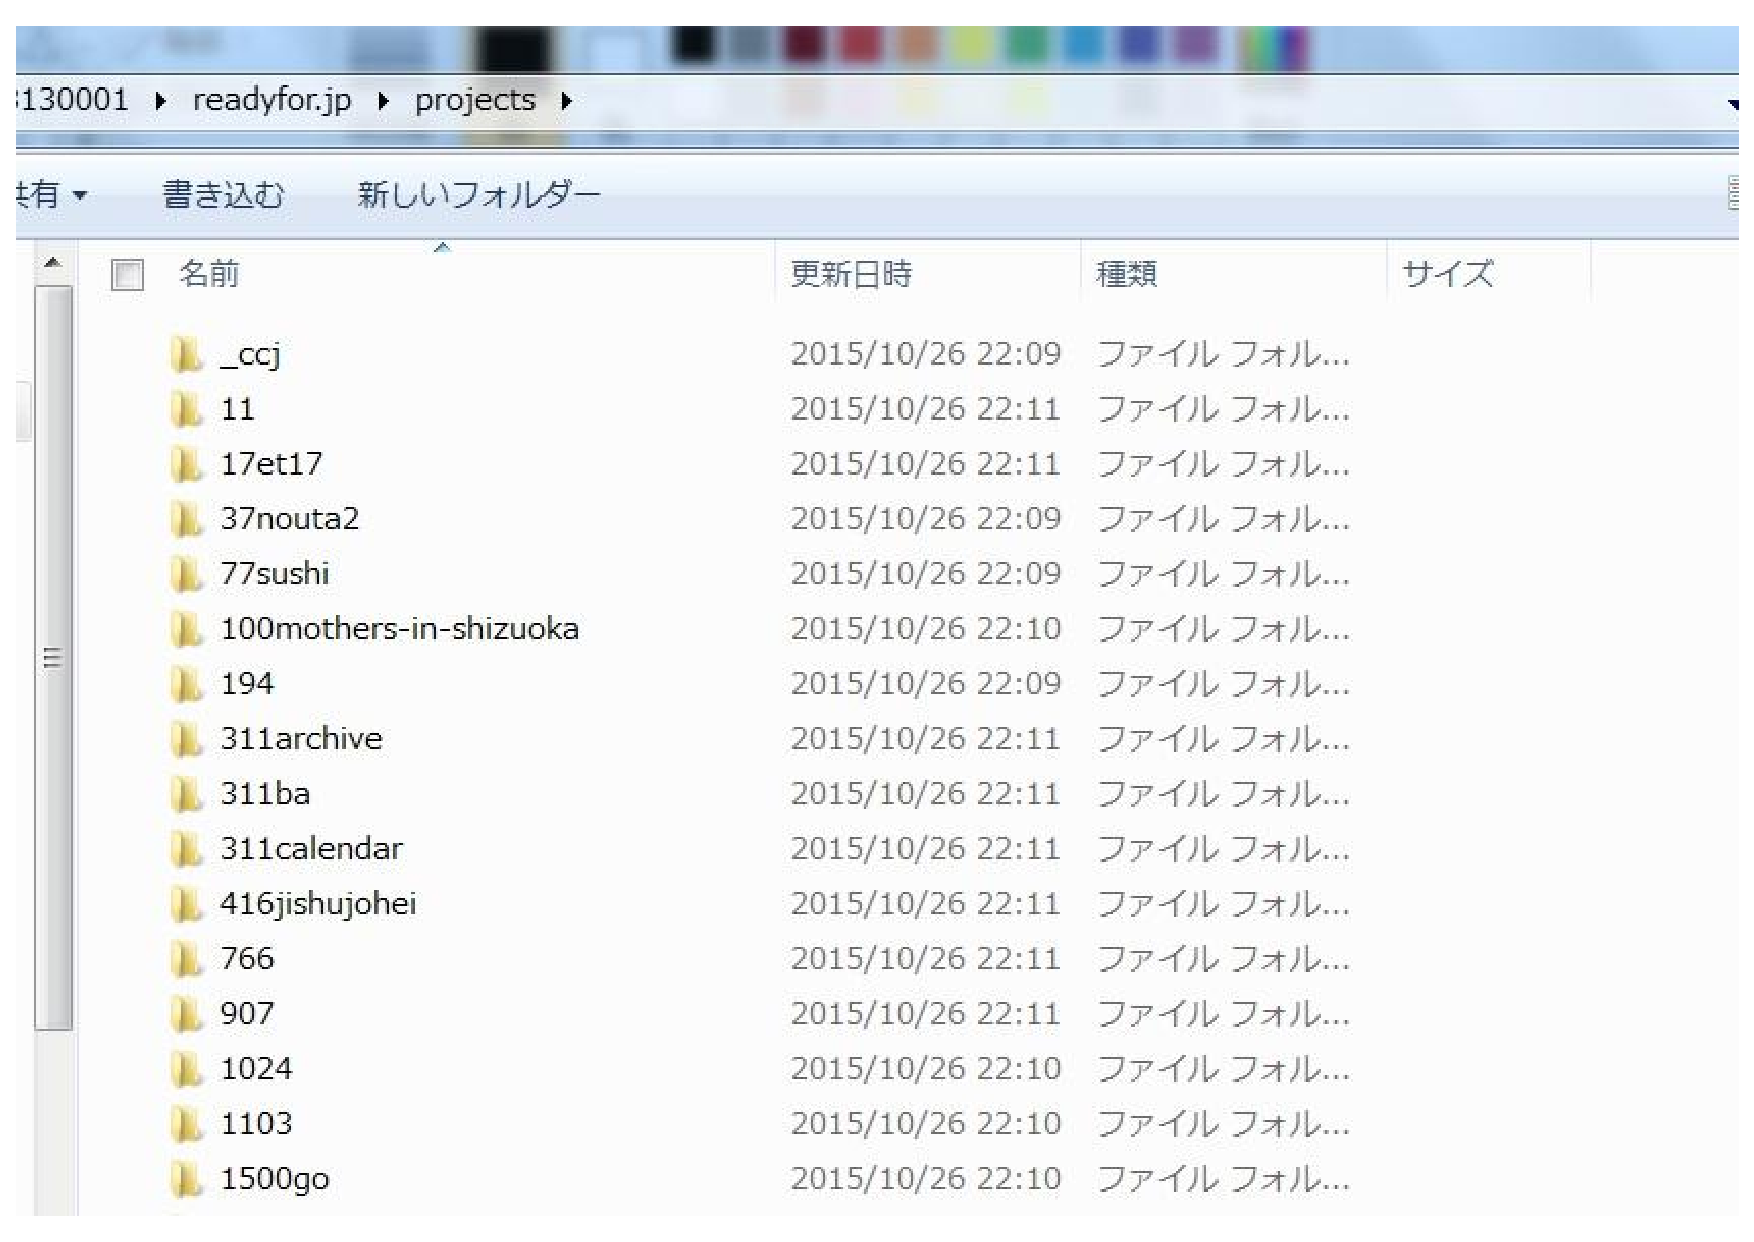
\includegraphics[width=13cm]{figure31.pdf}
\caption{READYFORのディレクトリ2}\label{sannp}
\end{figure}

READYFORのフォルダ内のprojectsフォルダ内に各プロジェクトごとにフォルダが存在する.


\begin{figure}[H]
\centering
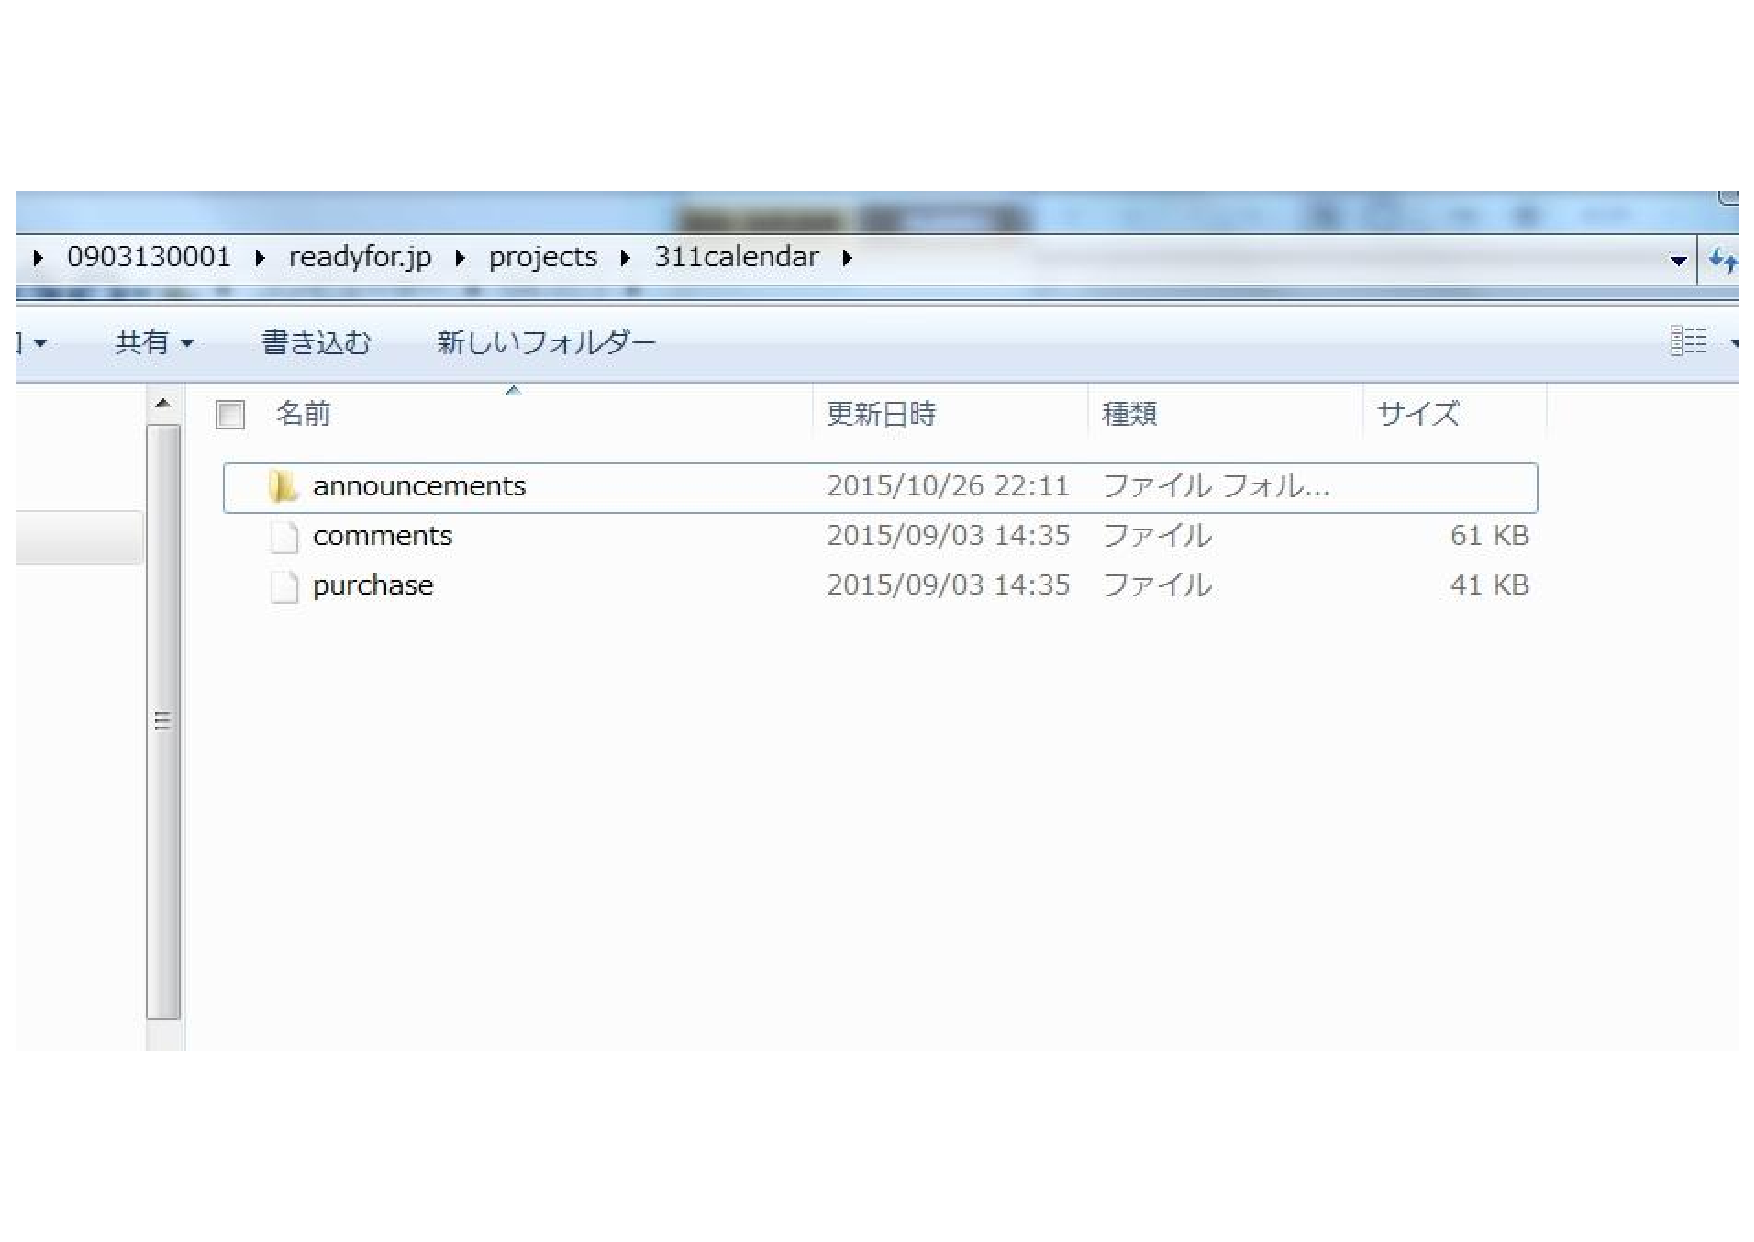
\includegraphics[width=13cm]{figure34.pdf}
\caption{READYFORのディレクトリ3}\label{sannp}
\end{figure}

\begin{figure}[H]
\centering
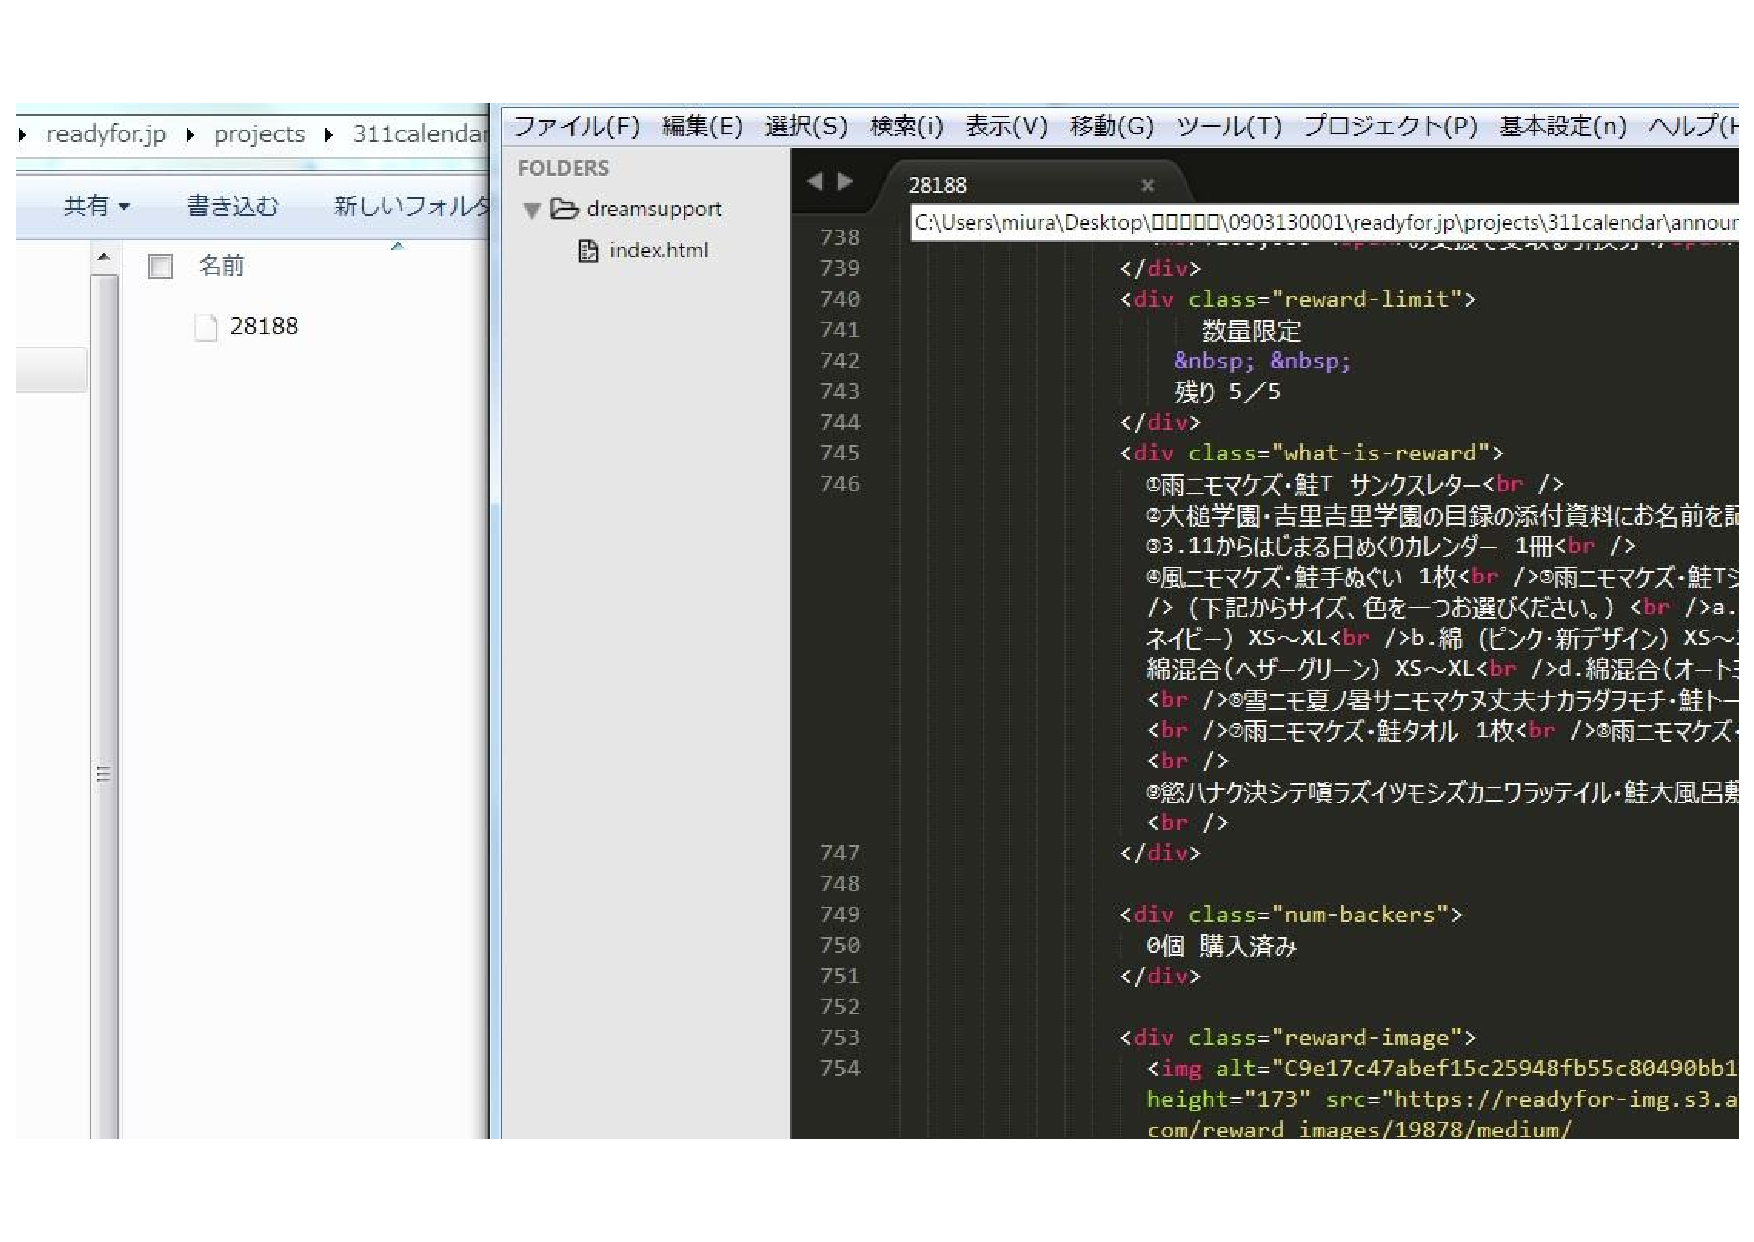
\includegraphics[width=13cm]{figure32.pdf}
\caption{READYFORのディレクトリ4}\label{sannp}
\end{figure}


プロジェクトフォルダ内にあるannouncementsフォルダの中にあるフォルダが各プロジェクトサイトのHTML文になっている.
テキストエディタなどによって開くことでHTML文から各プロジェクトの情報を知ることができる.

\begin{figure}[H]
\centering
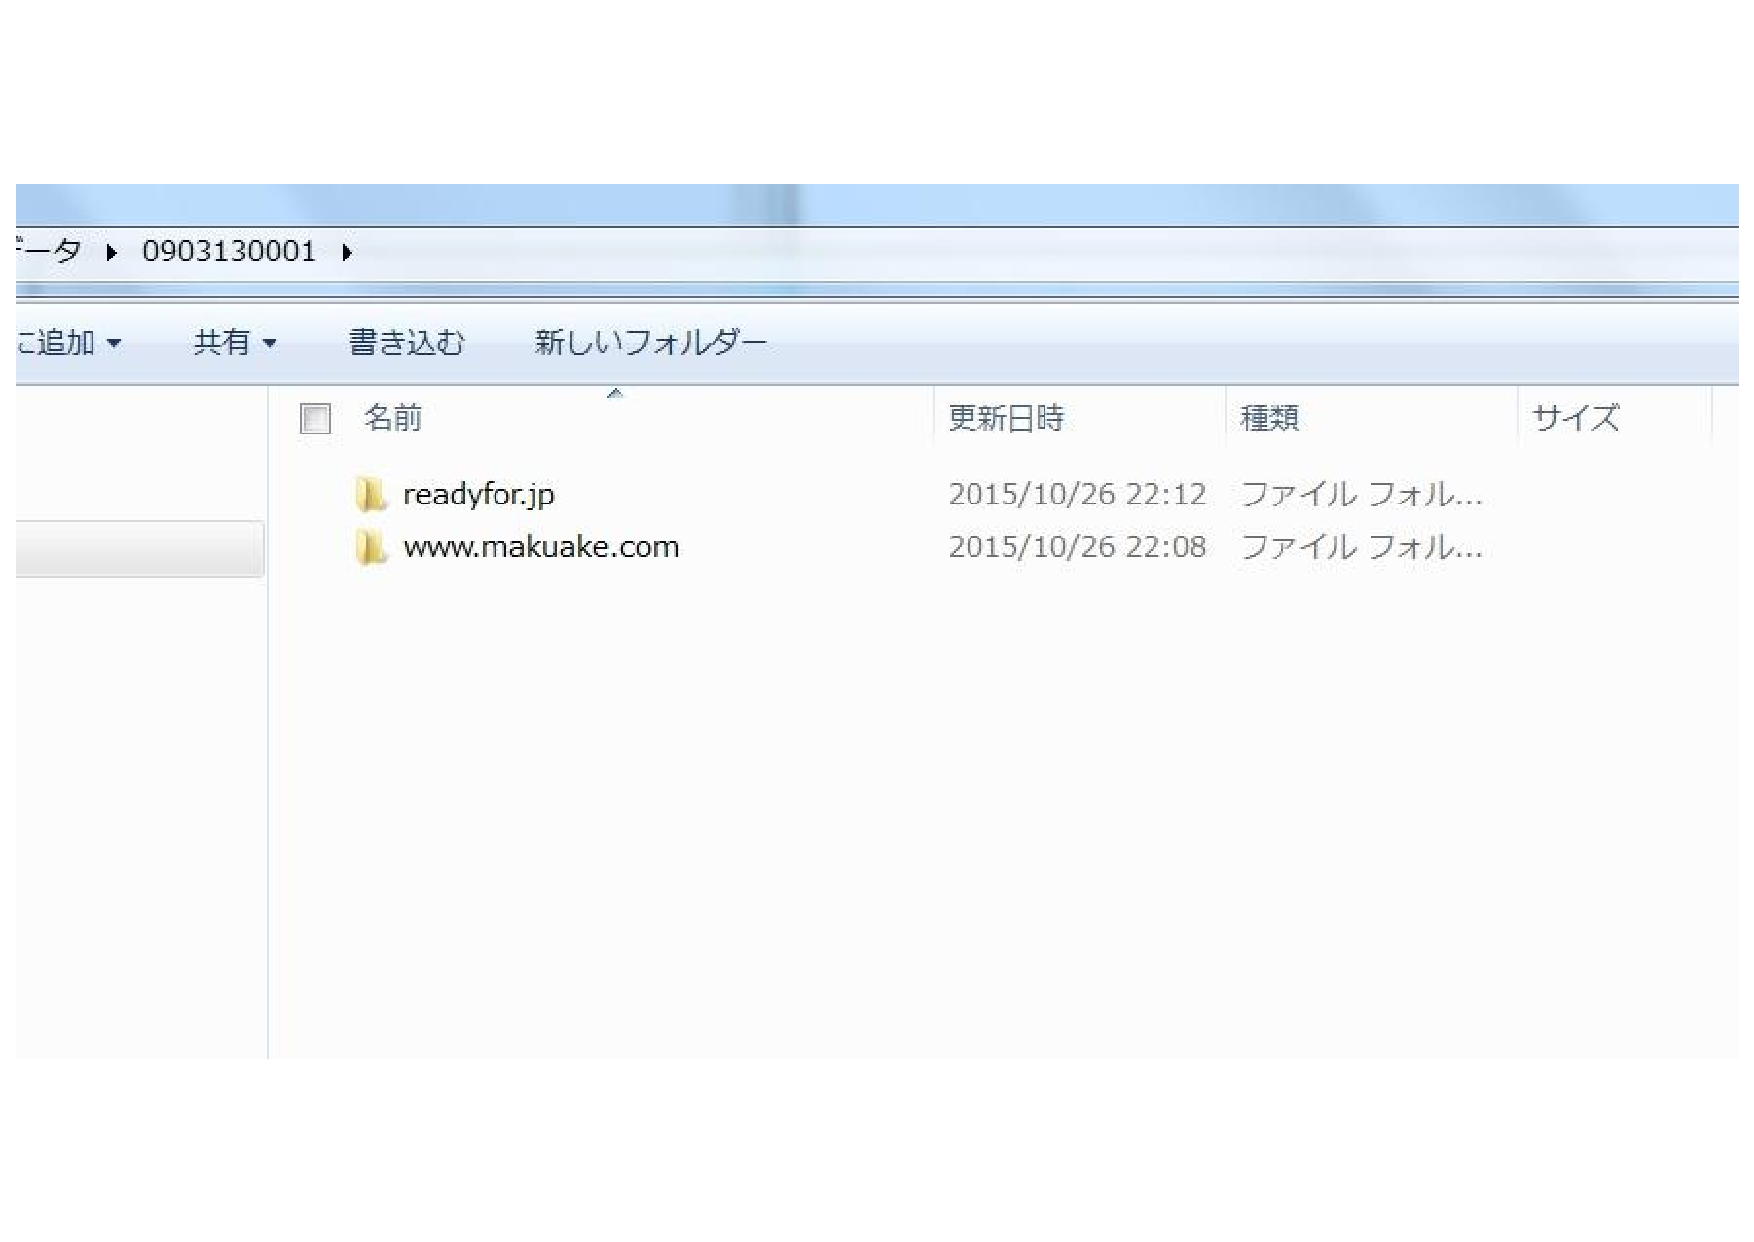
\includegraphics[width=13cm]{figure33.pdf}
\caption{実際のディレクトリ2}\label{sannp}
\end{figure}

次にMakuakeのディレクトリの説明を行う,Makuakeのフォルダ内のprojectフォルダ内に各プロジェクトごとにフォルダが形成されている.
またhttps://www.makuake.com/project/のあとにフォルダ名を足して検索することでインターネットに掲載されている状態のプロジェクトを見ることができる.

\begin{figure}[H]
\centering
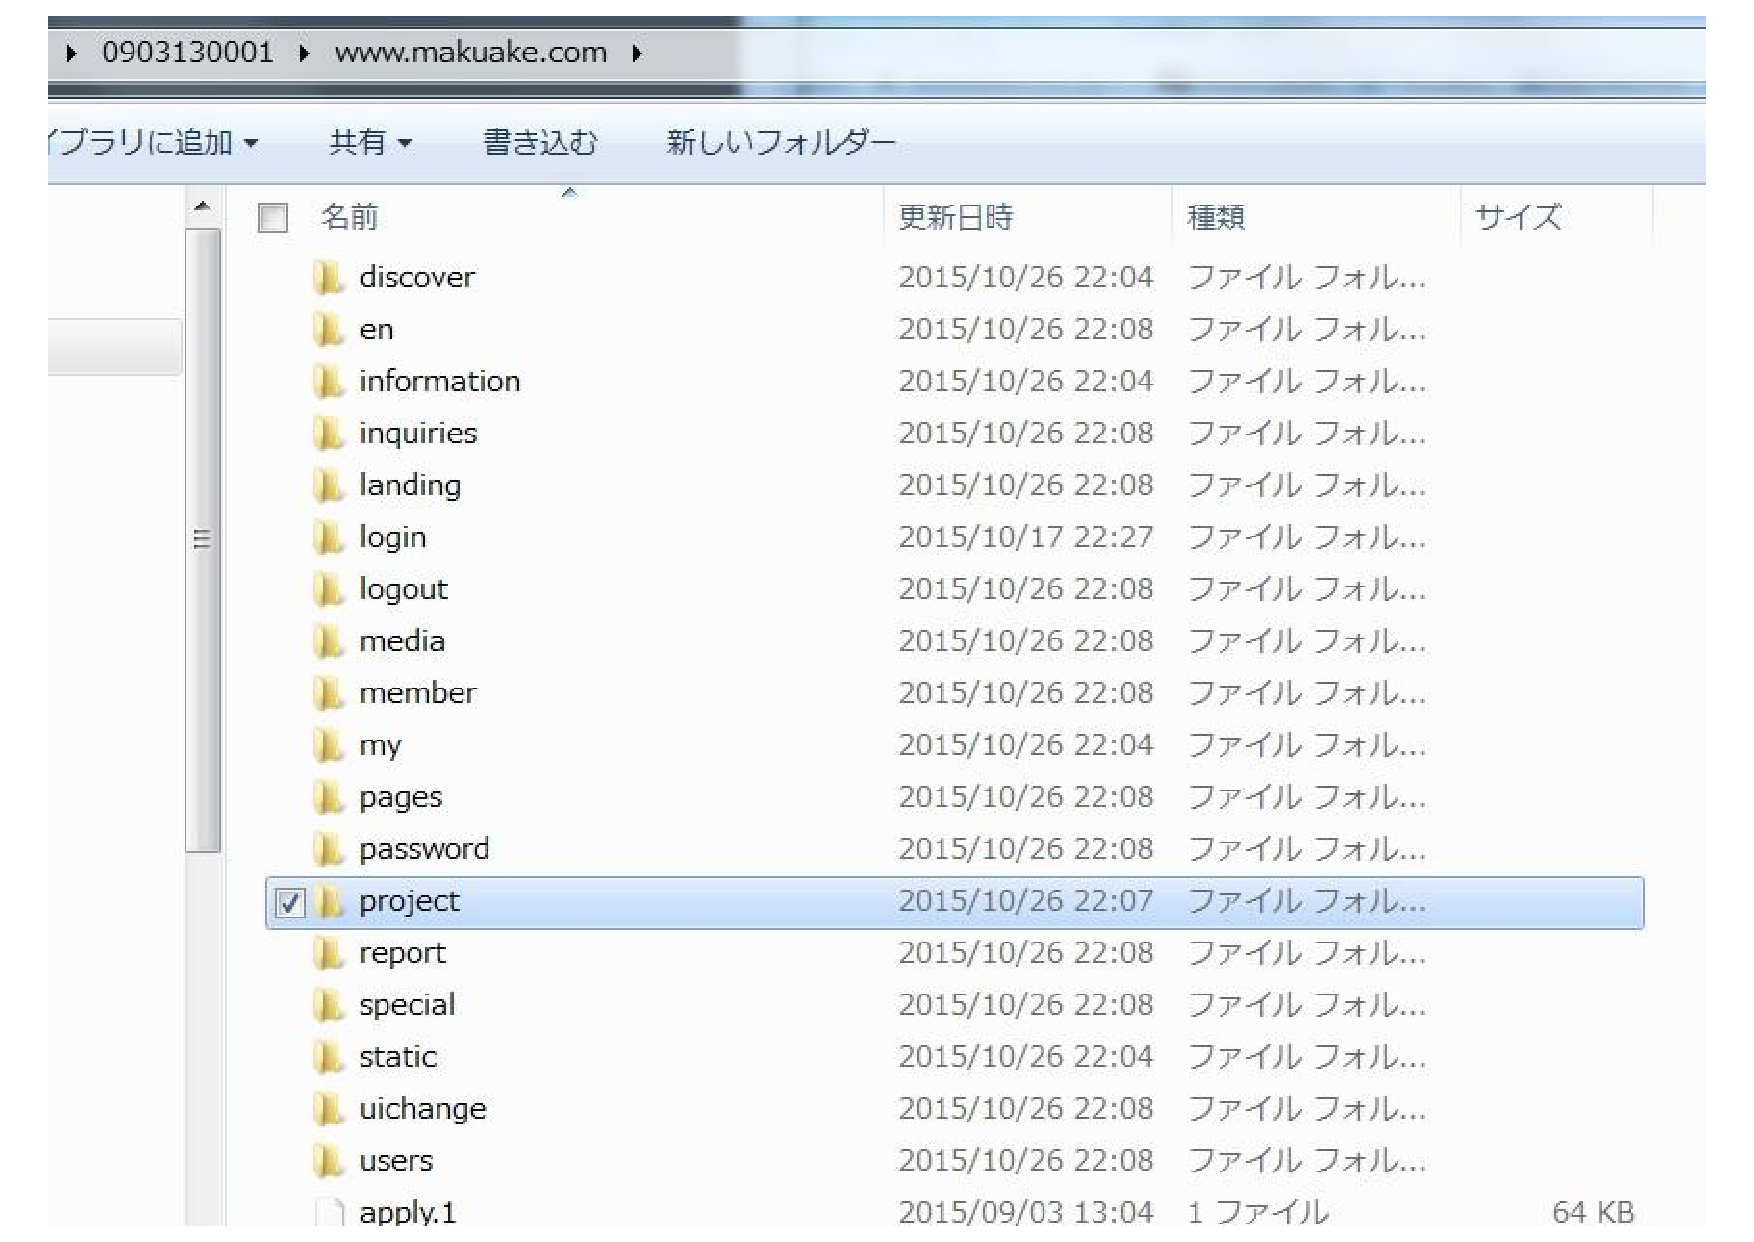
\includegraphics[width=13cm]{figure35.pdf}
\caption{Makuakeのディレクトリ1}\label{sannp}
\end{figure}

\begin{figure}[H]
\centering
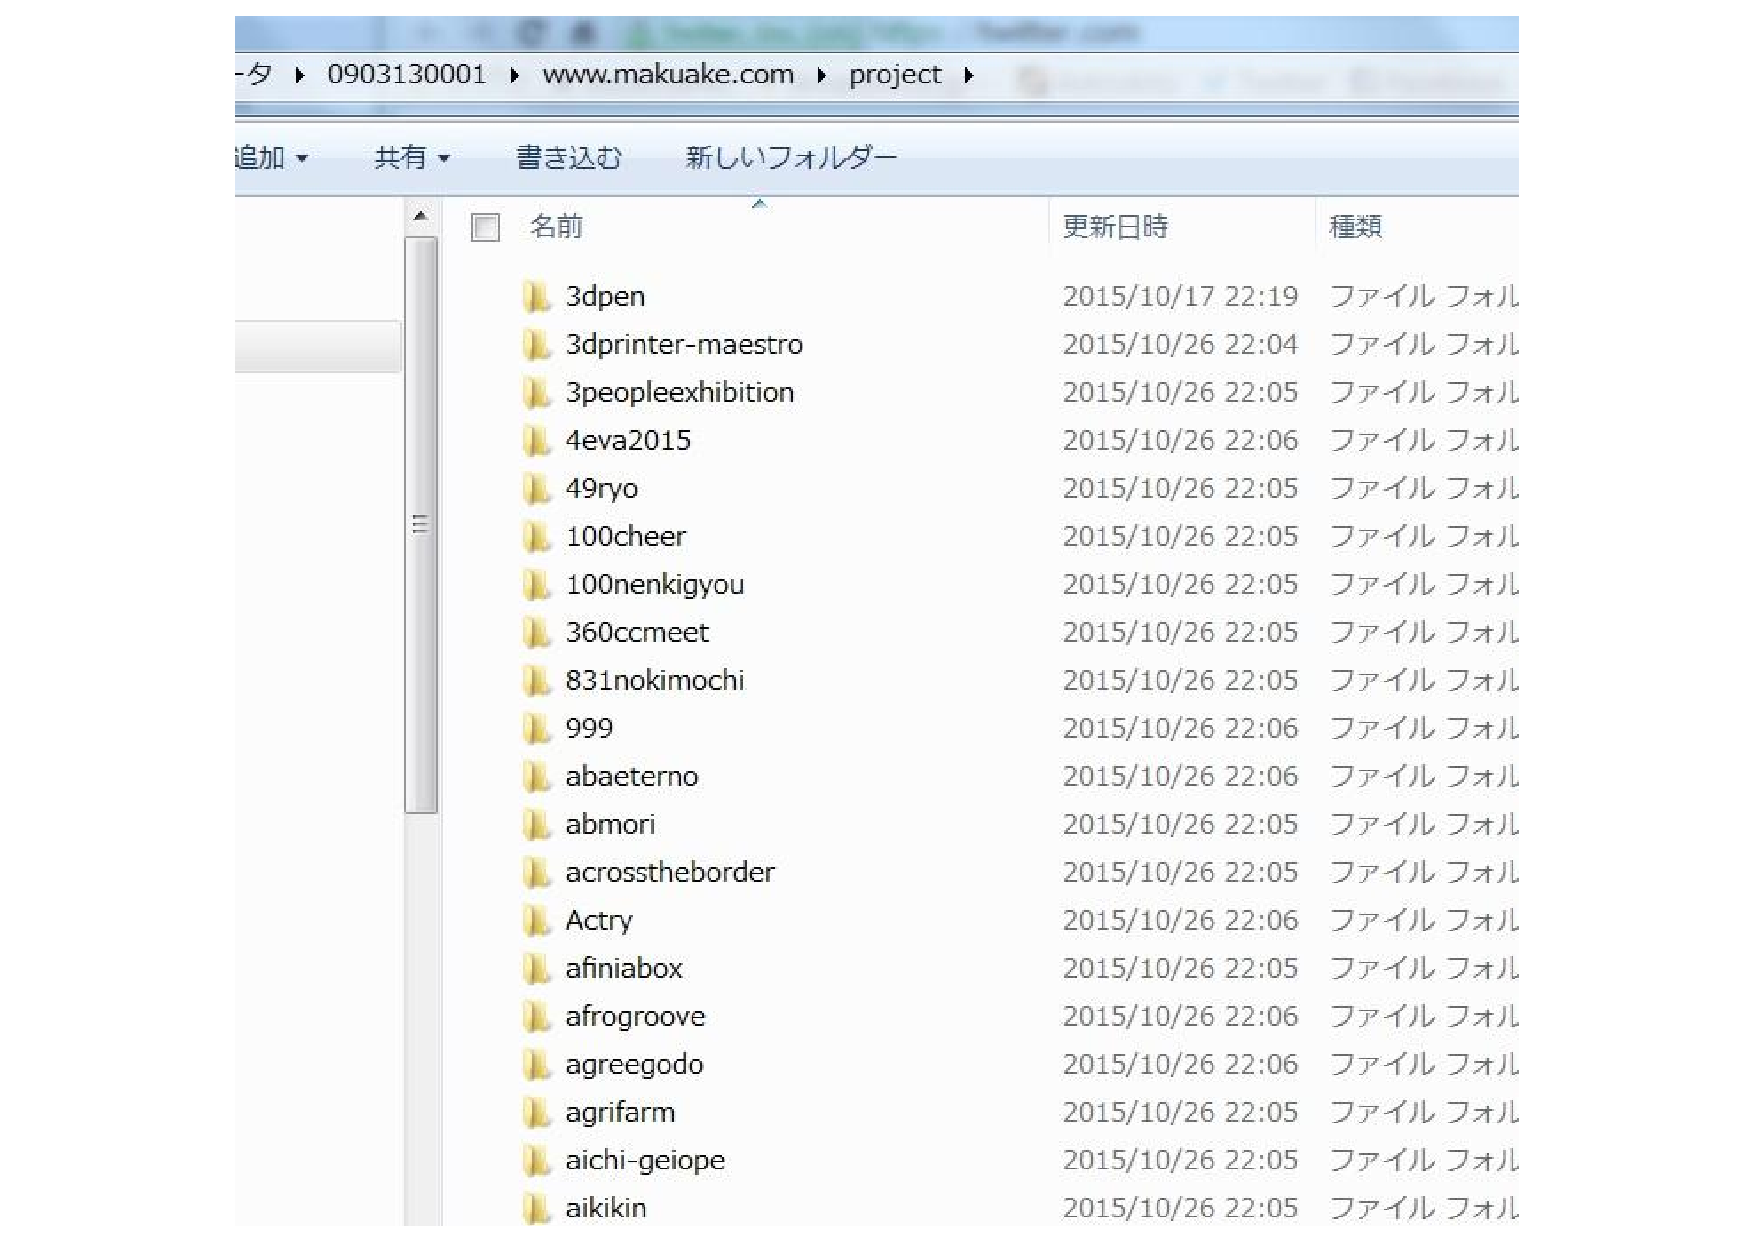
\includegraphics[width=13cm]{figure36.pdf}
\caption{Makuakeのディレクトリ2}\label{sannp}
\end{figure}

各プロジェクトフォルダの中にあるindex.htmlがHTML文になっておりテキストエディタやブラウザによって開くことができ,プロジェクトの情報を確認することができる.

\begin{figure}[H]
\centering
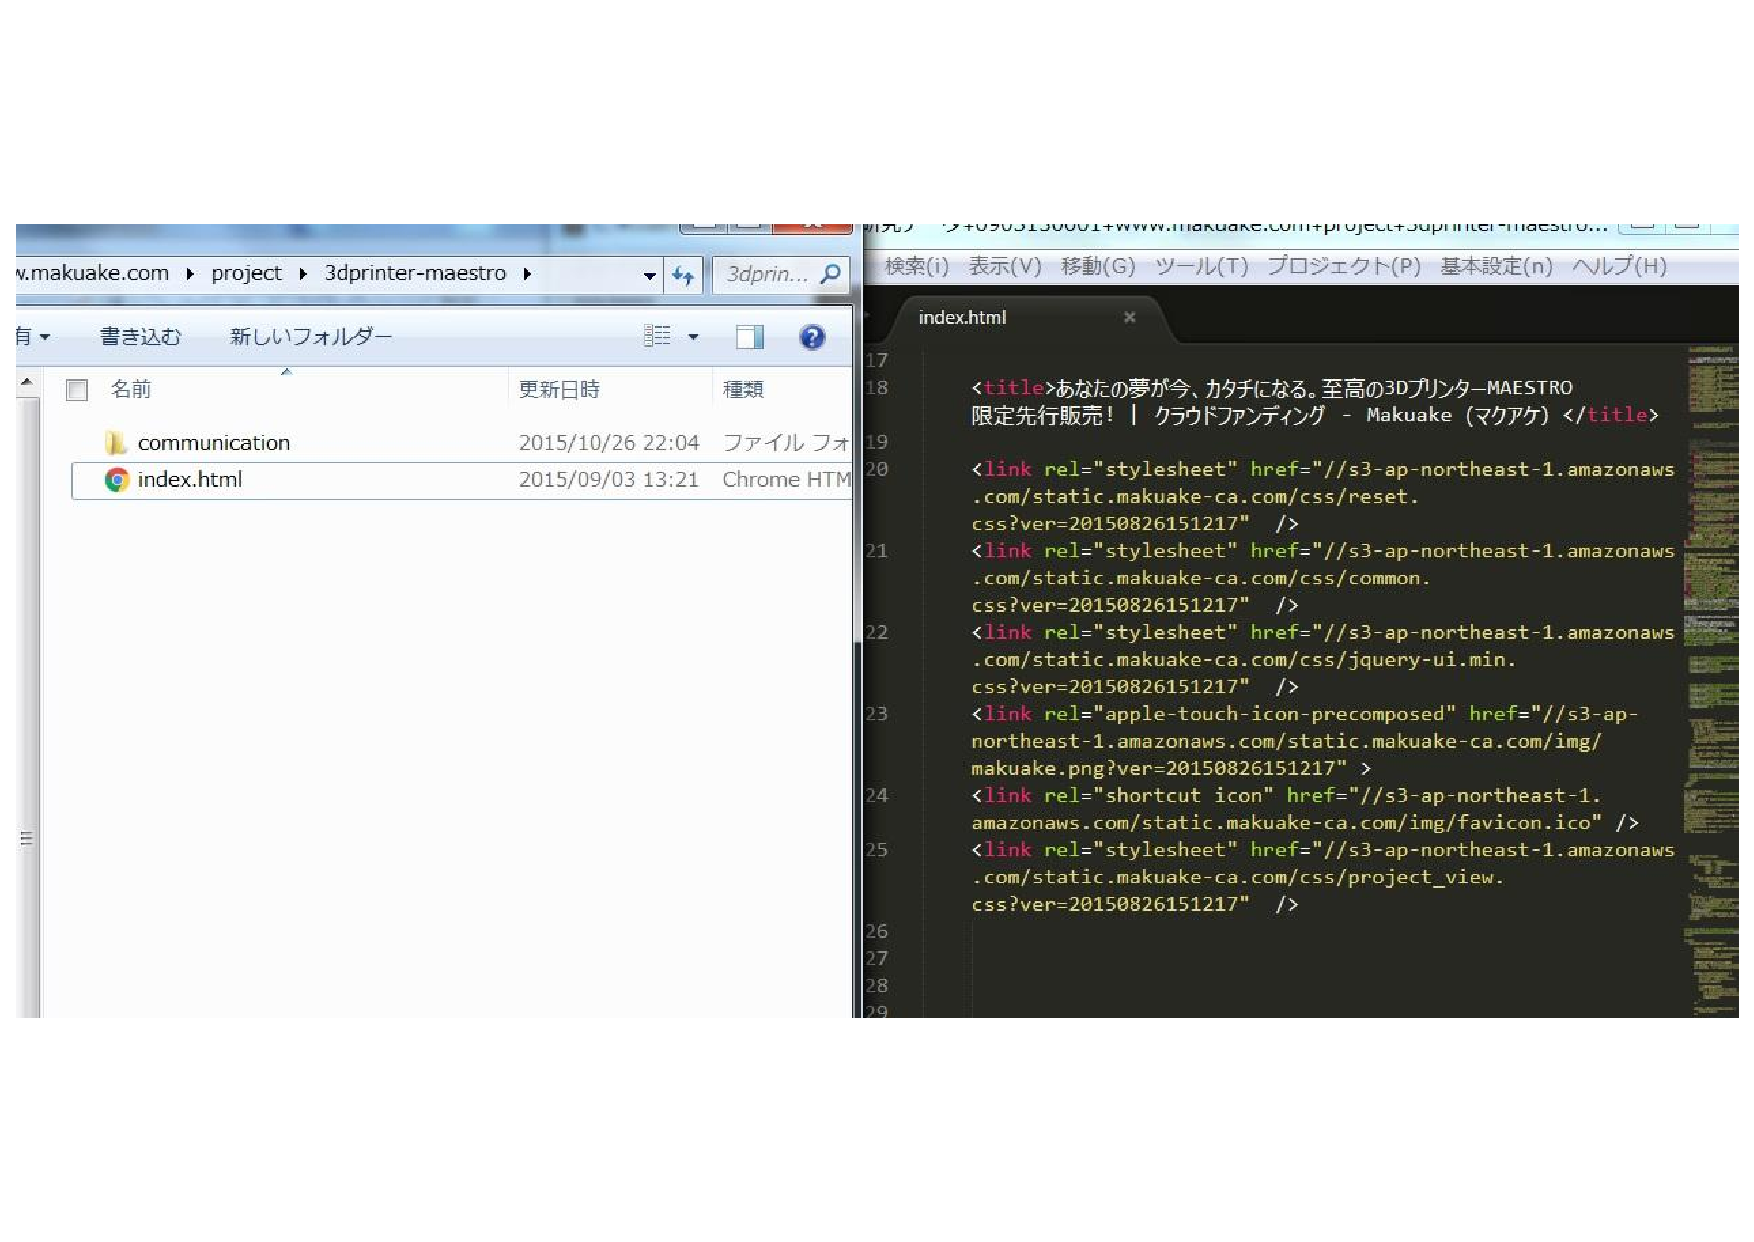
\includegraphics[width=13cm]{figure37.pdf}
\caption{Makuakeのディレクトリ3}\label{sannp}
\end{figure}




\chapter{判別分析について}

\section{使用したデータについて}

クローラーによって得られたデータを元に手作業で必要な要因を抽出していく,今回抽出した要因は目標金額・支援コース数・支援最低金
額・支援最高金額・リターンの有無・動画の有無・成功合否である.実際のデータの一部を以下に掲載する.

\begin{figure}[H]
\centering
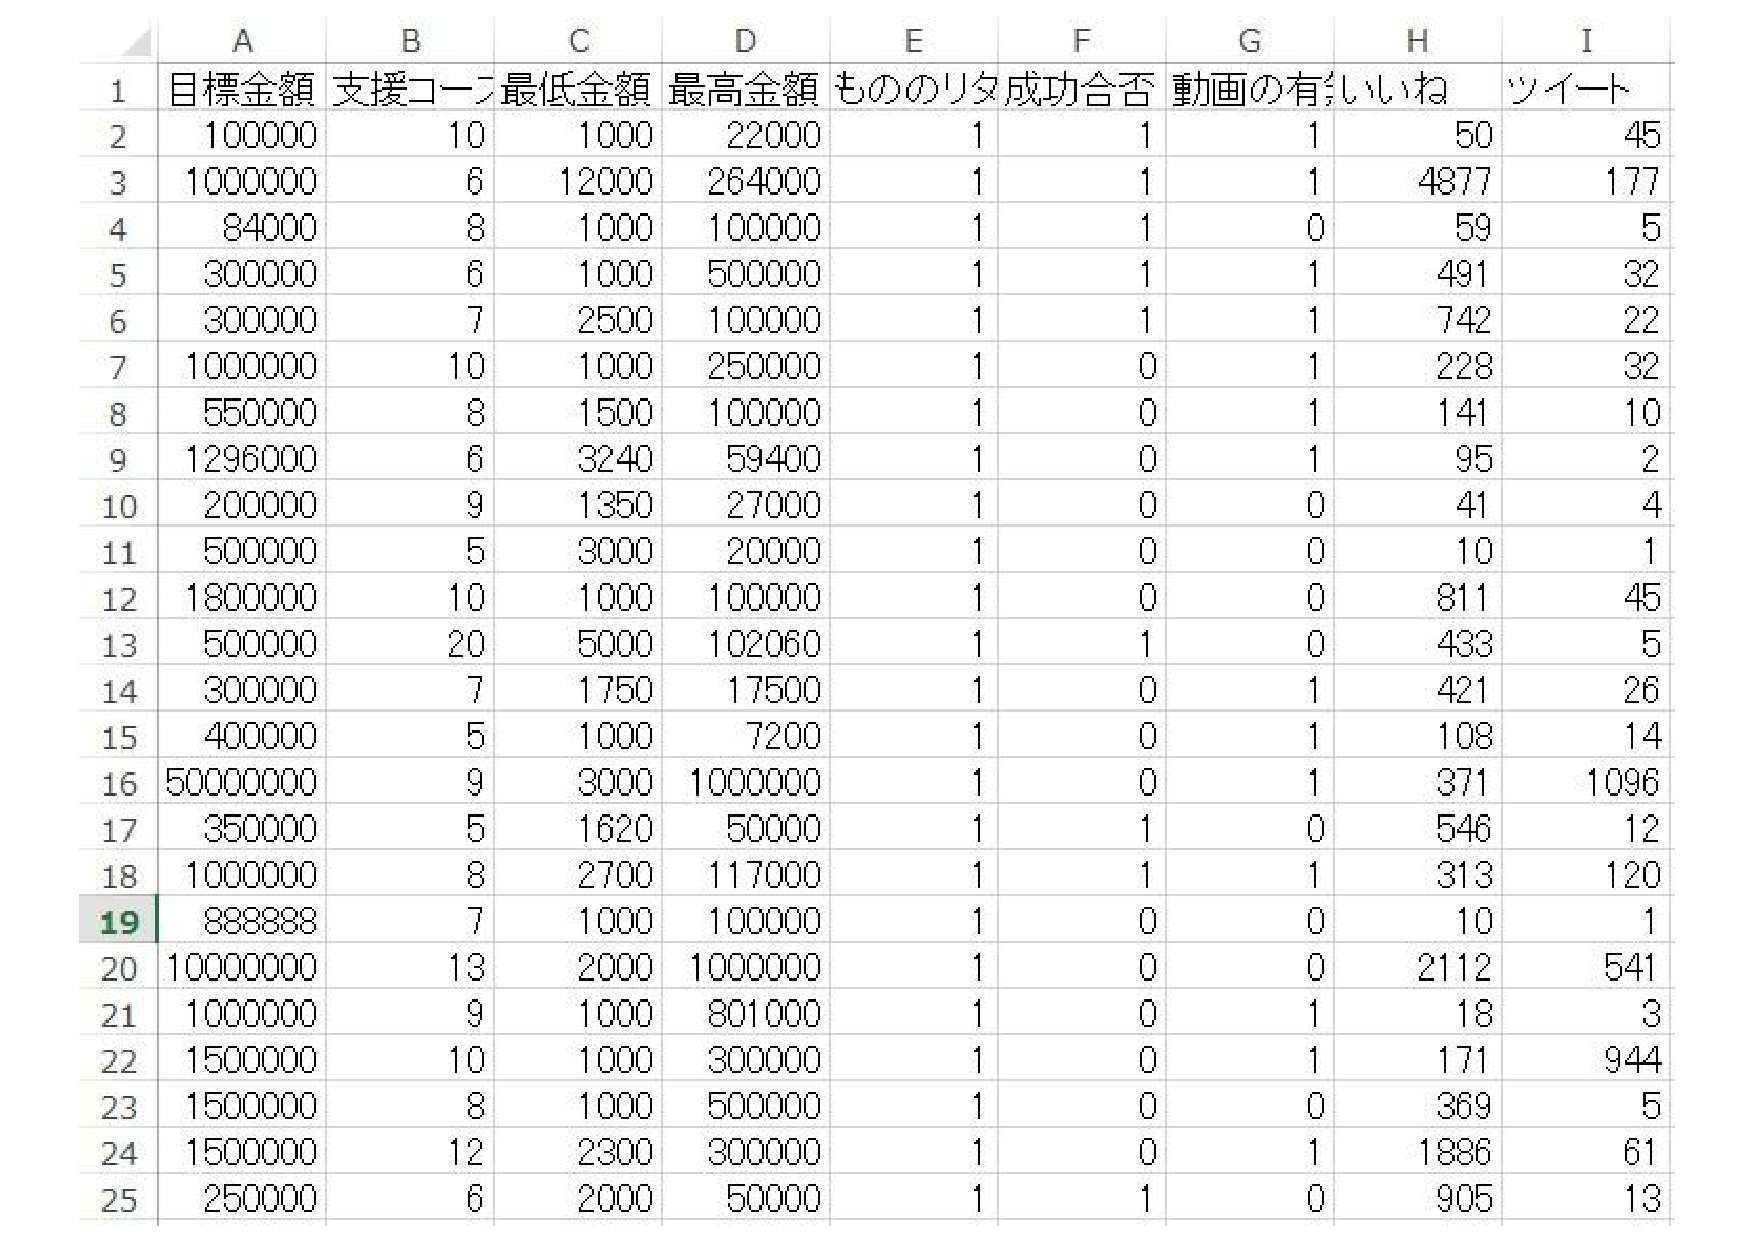
\includegraphics[width=13cm]{figure18.pdf}
\caption{使用したデータ}\label{sannp}
\end{figure}

今回は無作為に選出した100件のプロジェクトデータから要因を抽出した.

\section{判別分析の手法}

今回,判別分析の手法である,ロジスティック回帰分析と決定木分析の二つから分析方法を選定する.
ロジスティック回帰分析は,入力が1と0やあり,なしなど相反するカテゴリを変数とするときに適した分析方法である.
係数などから要因の関係性を追及することなどが可能であり,詳しい成果などを得ることがしやすい.

決定木分析は,目的変数を説明する変数がなにか決定木を描くことにより考察することができる手法である.

ロジスティック回帰分析のほうが詳しい成果を得やすいと書きながら決定木分析を選ぶ理由として
\begin{itemize}
\item 関係のありそうな要因が捕らえにくく,まったく関係ないものとそうでないものの基準がなにもないため.
 \item 結果を視覚的で捕らえやすく考察しやすい.
 \item クラウドファンディングを行う際,得られた決定木を使用することができる.

\end{itemize}

ことをあげる.今回の結果を元にロジスティック回帰分析を行うことでさらに詳しい成果を得ることができると考える.

\section{決定木分析について}

決定木分析とは,教師あり学習のわかりやすいものとしてあげられ,決定木を描くことで目的変数を説明する要因が何か考察することができる手法である.結果が見やすくデータマイニングに慣れてない人からも受け入れやすいのが特徴である.

矛盾するデータが無い場合は,決定木を作ることができる.下記に記した学生の生活から決定木を描いた.

\begin{figure}[H]
\centering
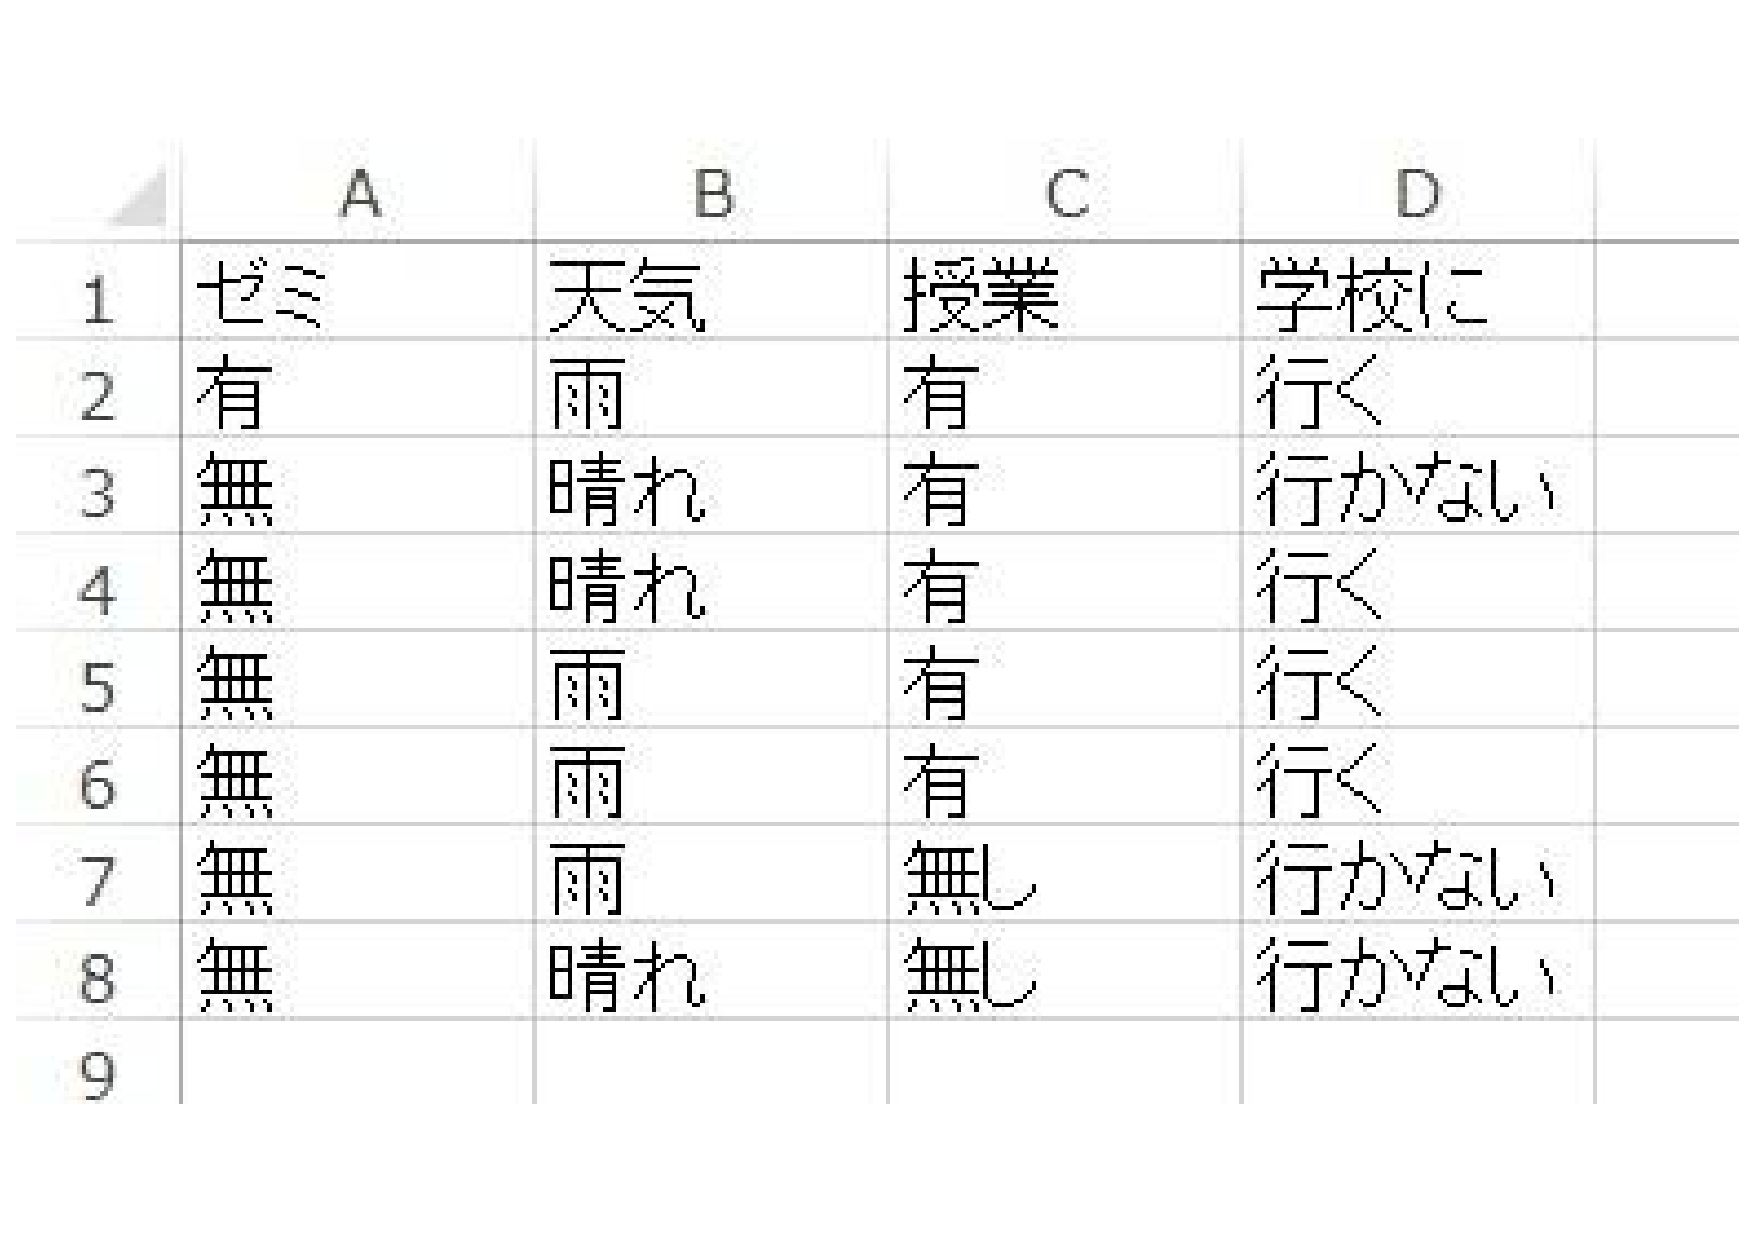
\includegraphics[width=13cm]{figure47.pdf}
\caption{決定木に使用するデータ}\label{sannp}
\end{figure}

\begin{figure}[H]
\centering
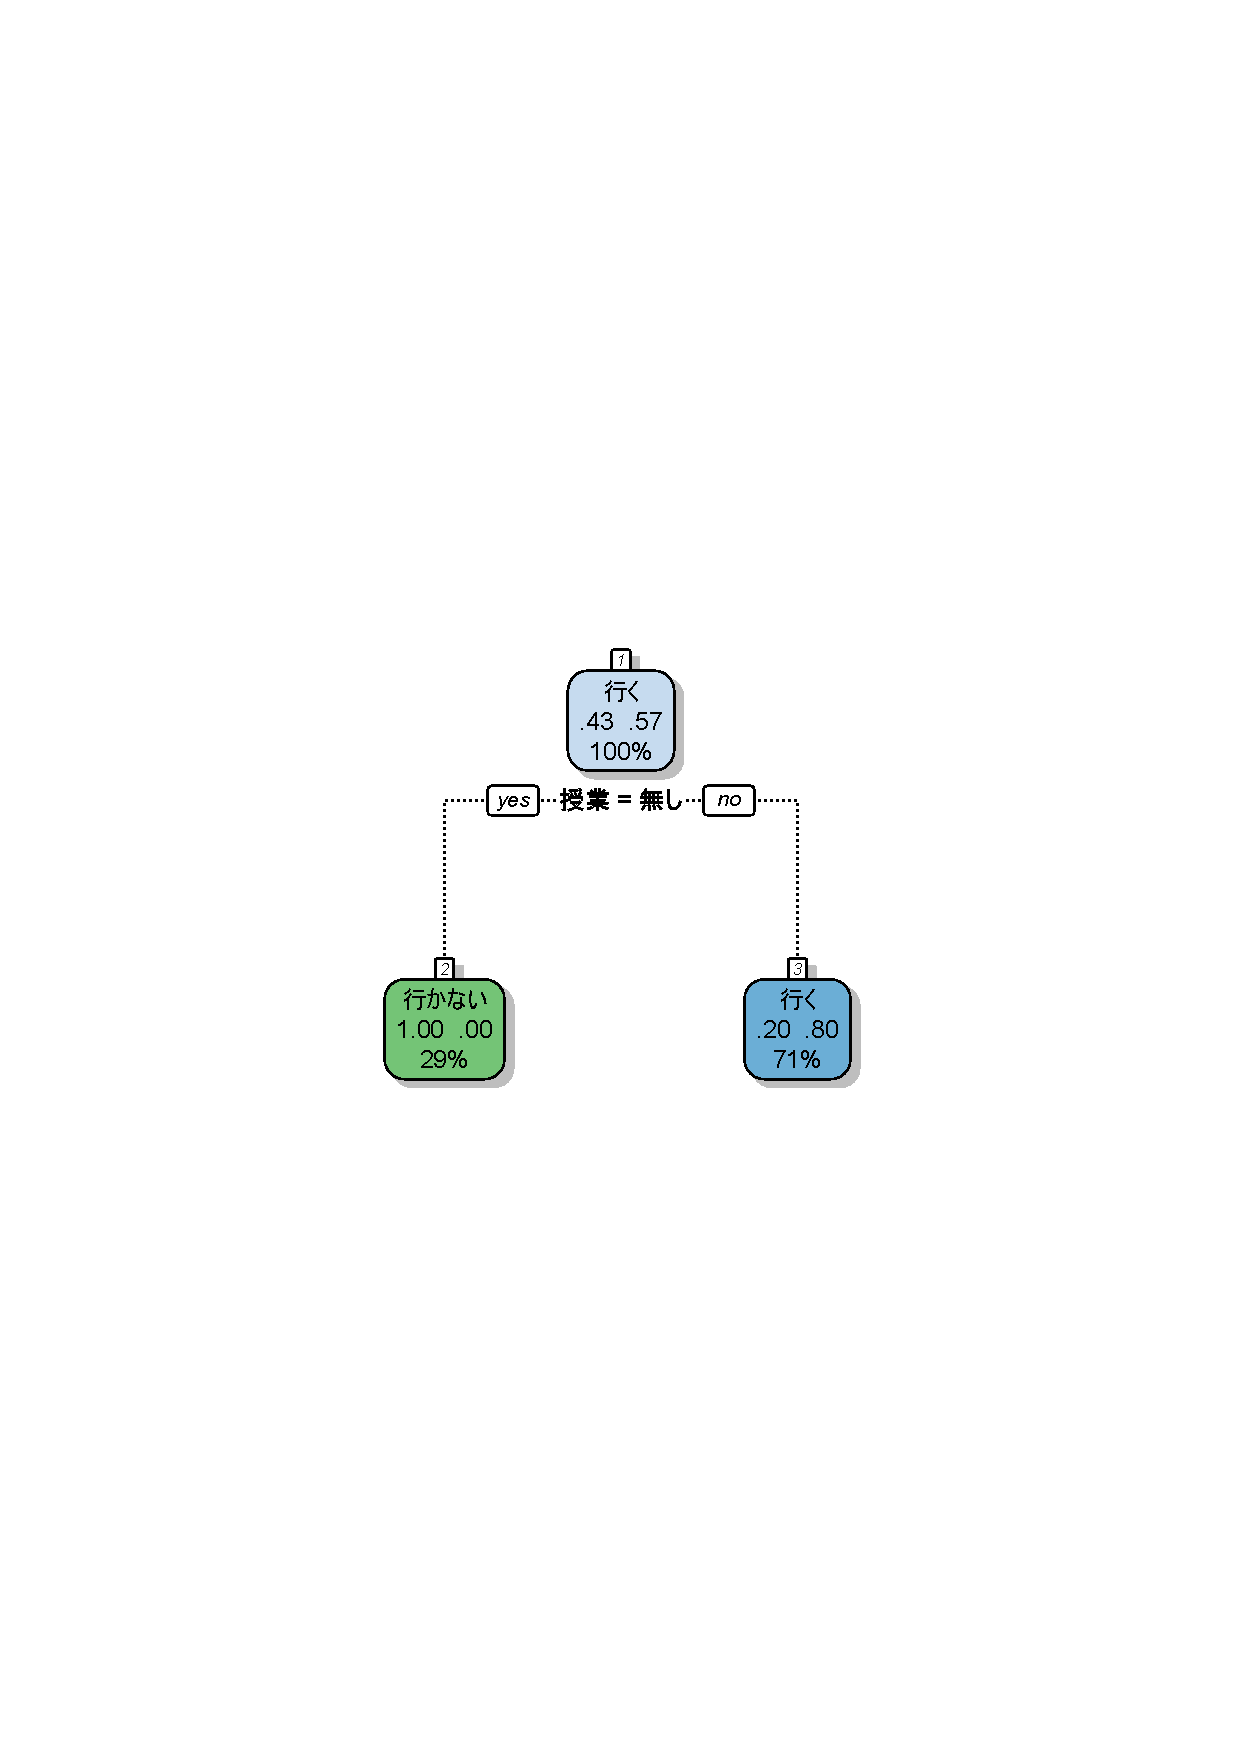
\includegraphics[width=13cm]{figure46.pdf}
\caption{決定木}\label{sannp}
\end{figure}

得られた決定木からこの学生は授業が無い日は学校には行かないことがわかる.また授業がある日はほとんどの場合は学校に行くが例外もあることが伺える.

決定木の善し悪しの基準は「簡潔な仮説がよい仮説である」というオッカムの剃刀の法則がよく言われる.ひとつのことを説明するときの変数が答えが同じであるならば変数の数は少ないほうがよい.

今回描いた決定木は短く適切な決定木といえる.



\section{決定木分析の手順}

Rで決定木分析を行う手順を本章では掲載する.
集めた要因をまとめcsvファイルにまとめ,Cドライブにcitという名前でフォルダを作成し,保存する.
なお,フォルダの名前は変えても大丈夫だが今回は説明のためにcitとする.

\begin{figure}[H]
\centering
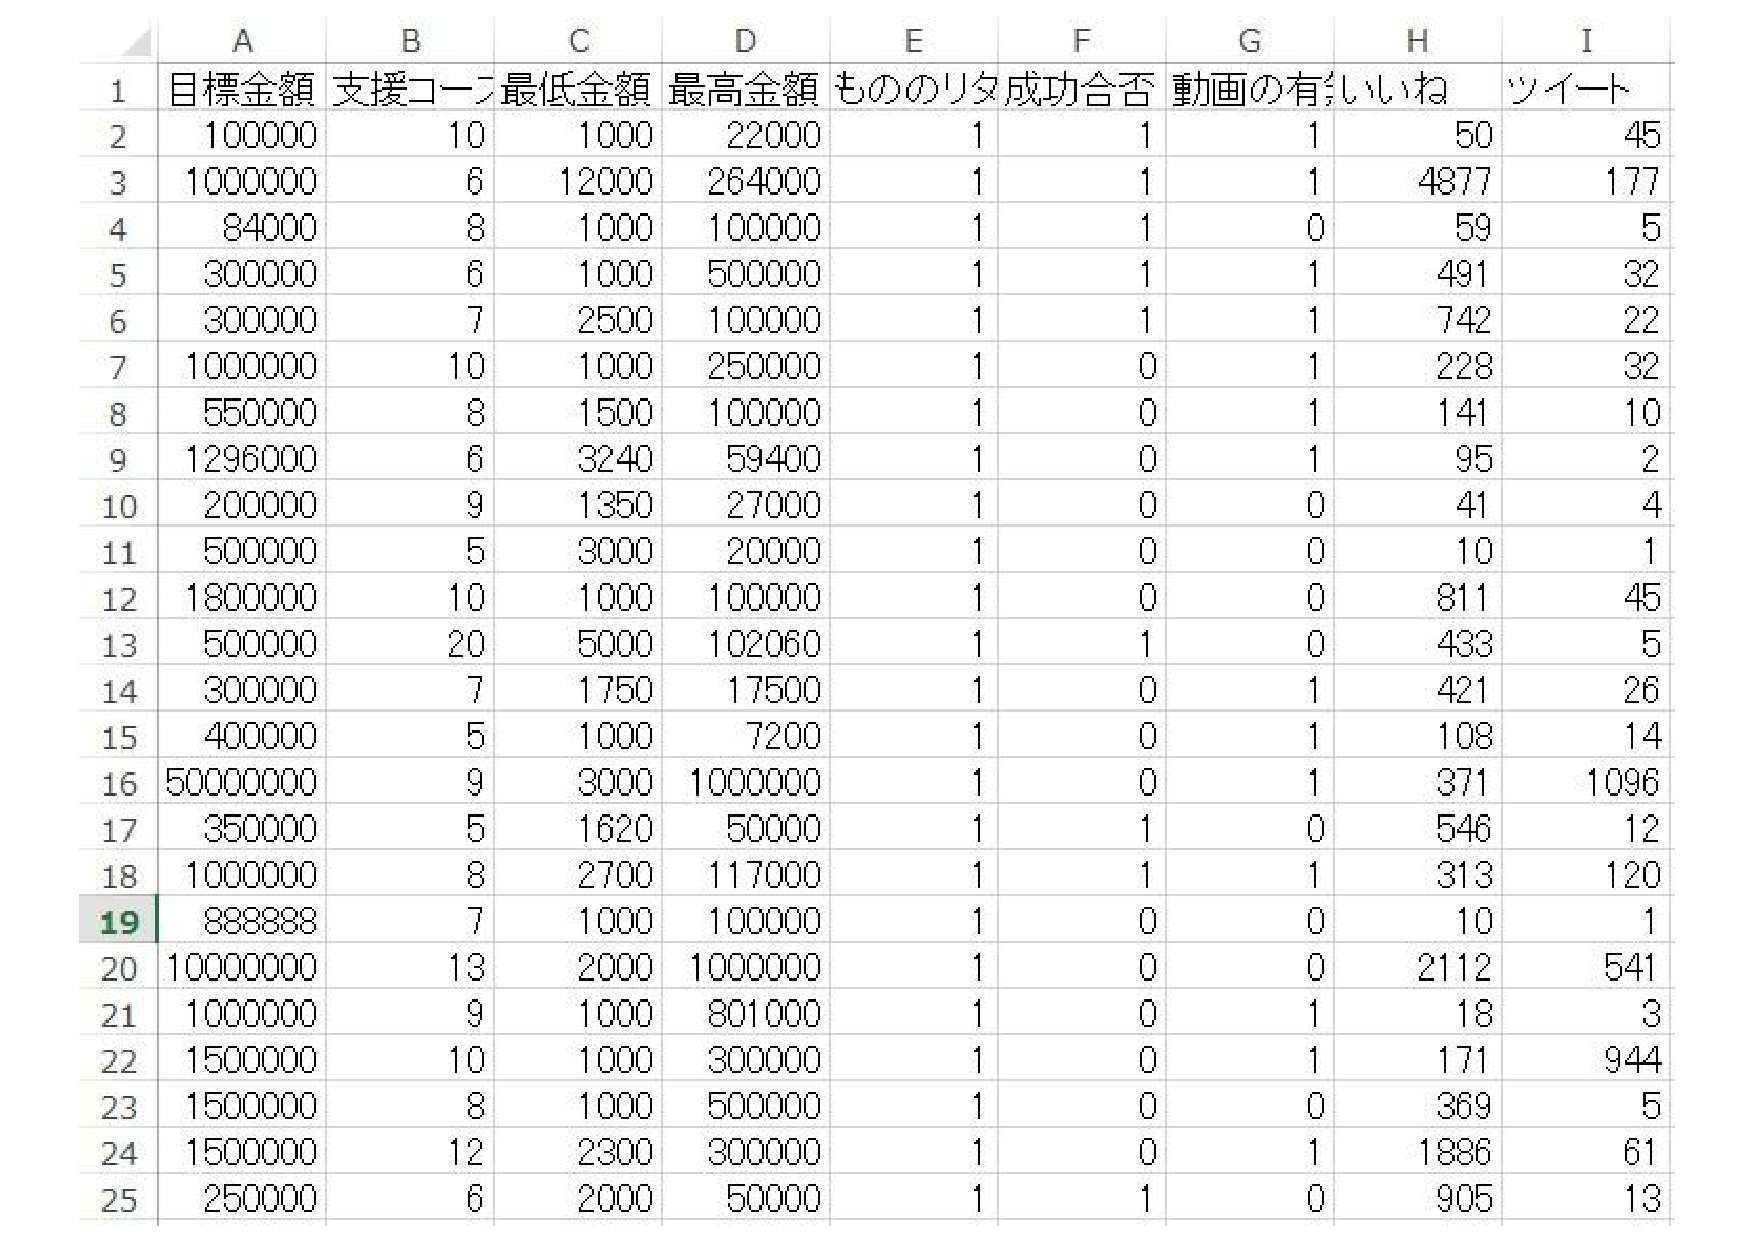
\includegraphics[width=13cm]{figure18.pdf}
\caption{使用したデータ}\label{sannp}
\end{figure}


\begin{figure}[H]
\centering
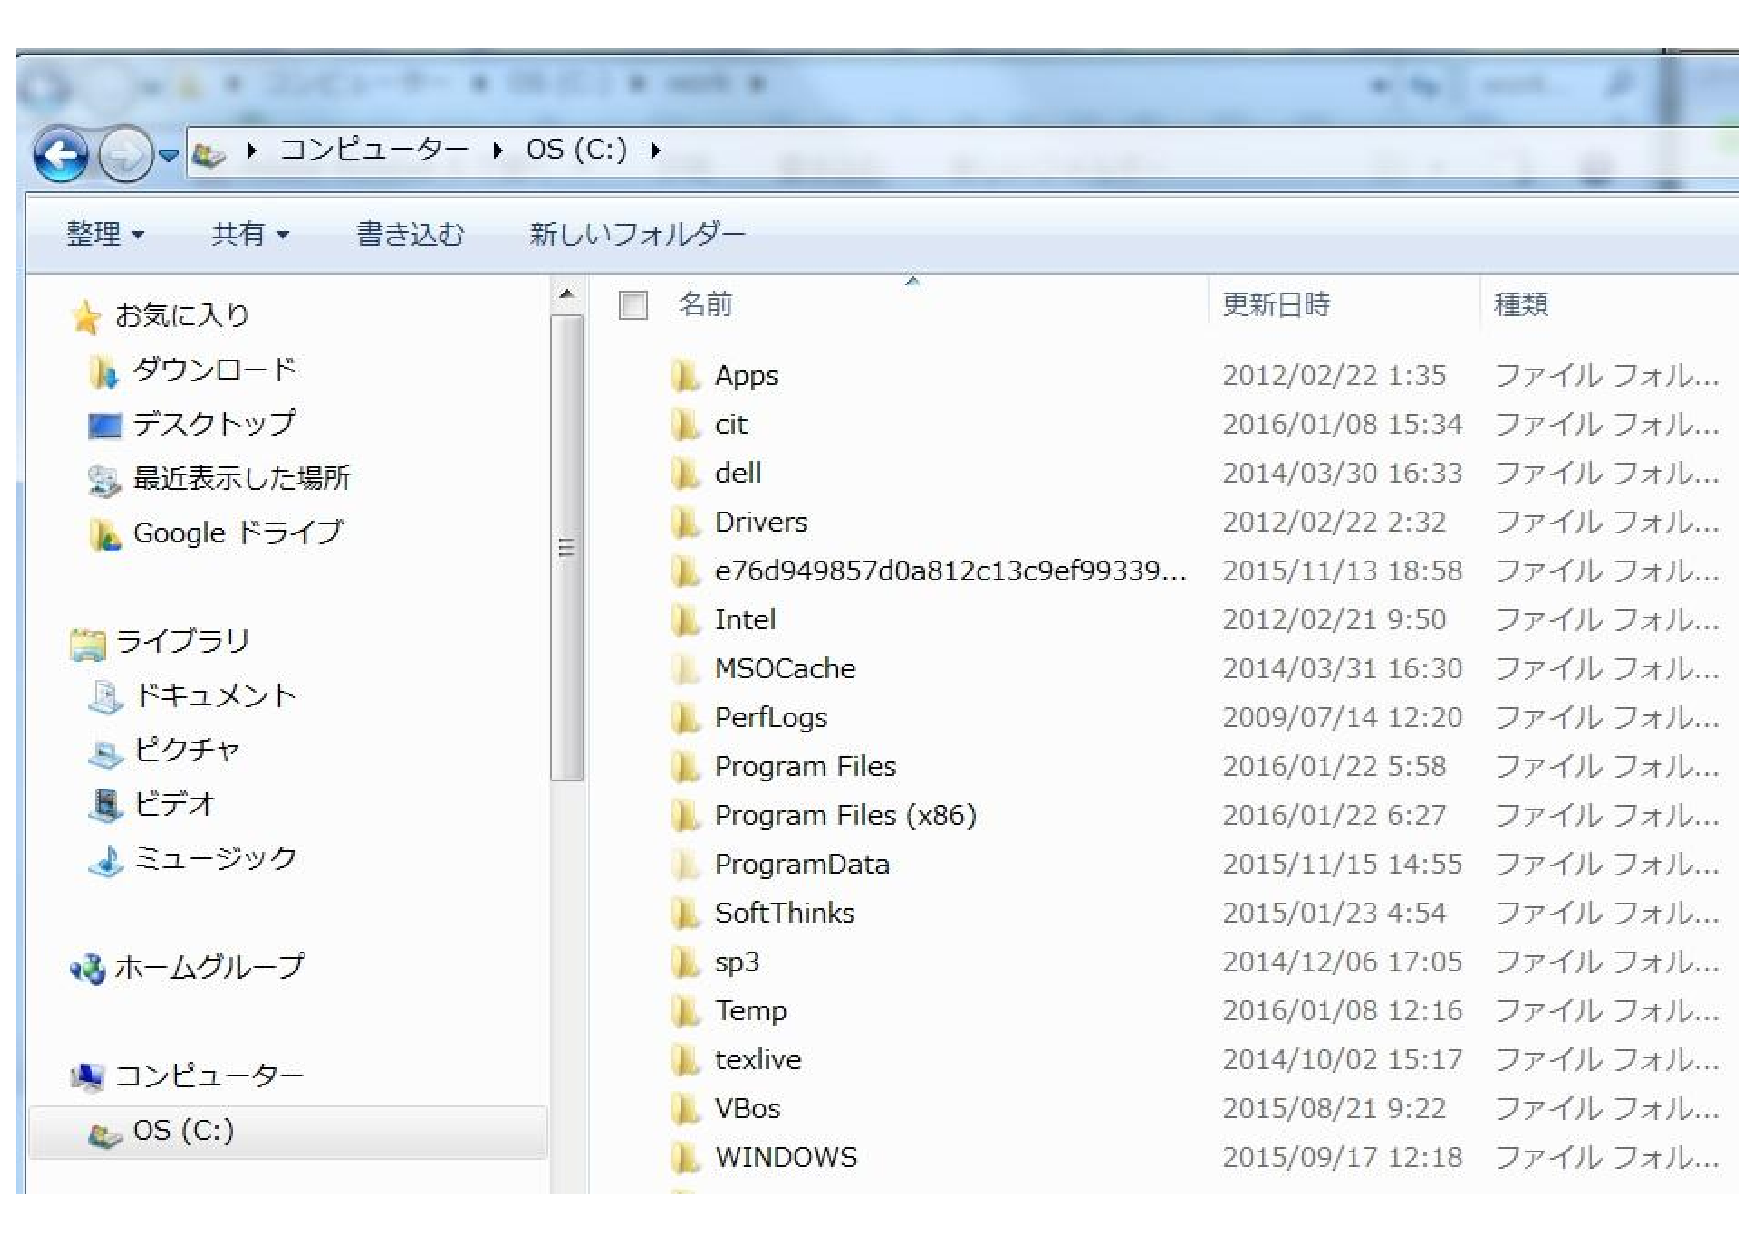
\includegraphics[width=10cm]{figure20.pdf}
\caption{フォルダを作成する}\label{sannp}
\end{figure}

また今回使用するデータの名前を仮にデータ.csvとする.
Rを起動し,以下のコマンドを命令する.


\begin{figure}[H]
\centering
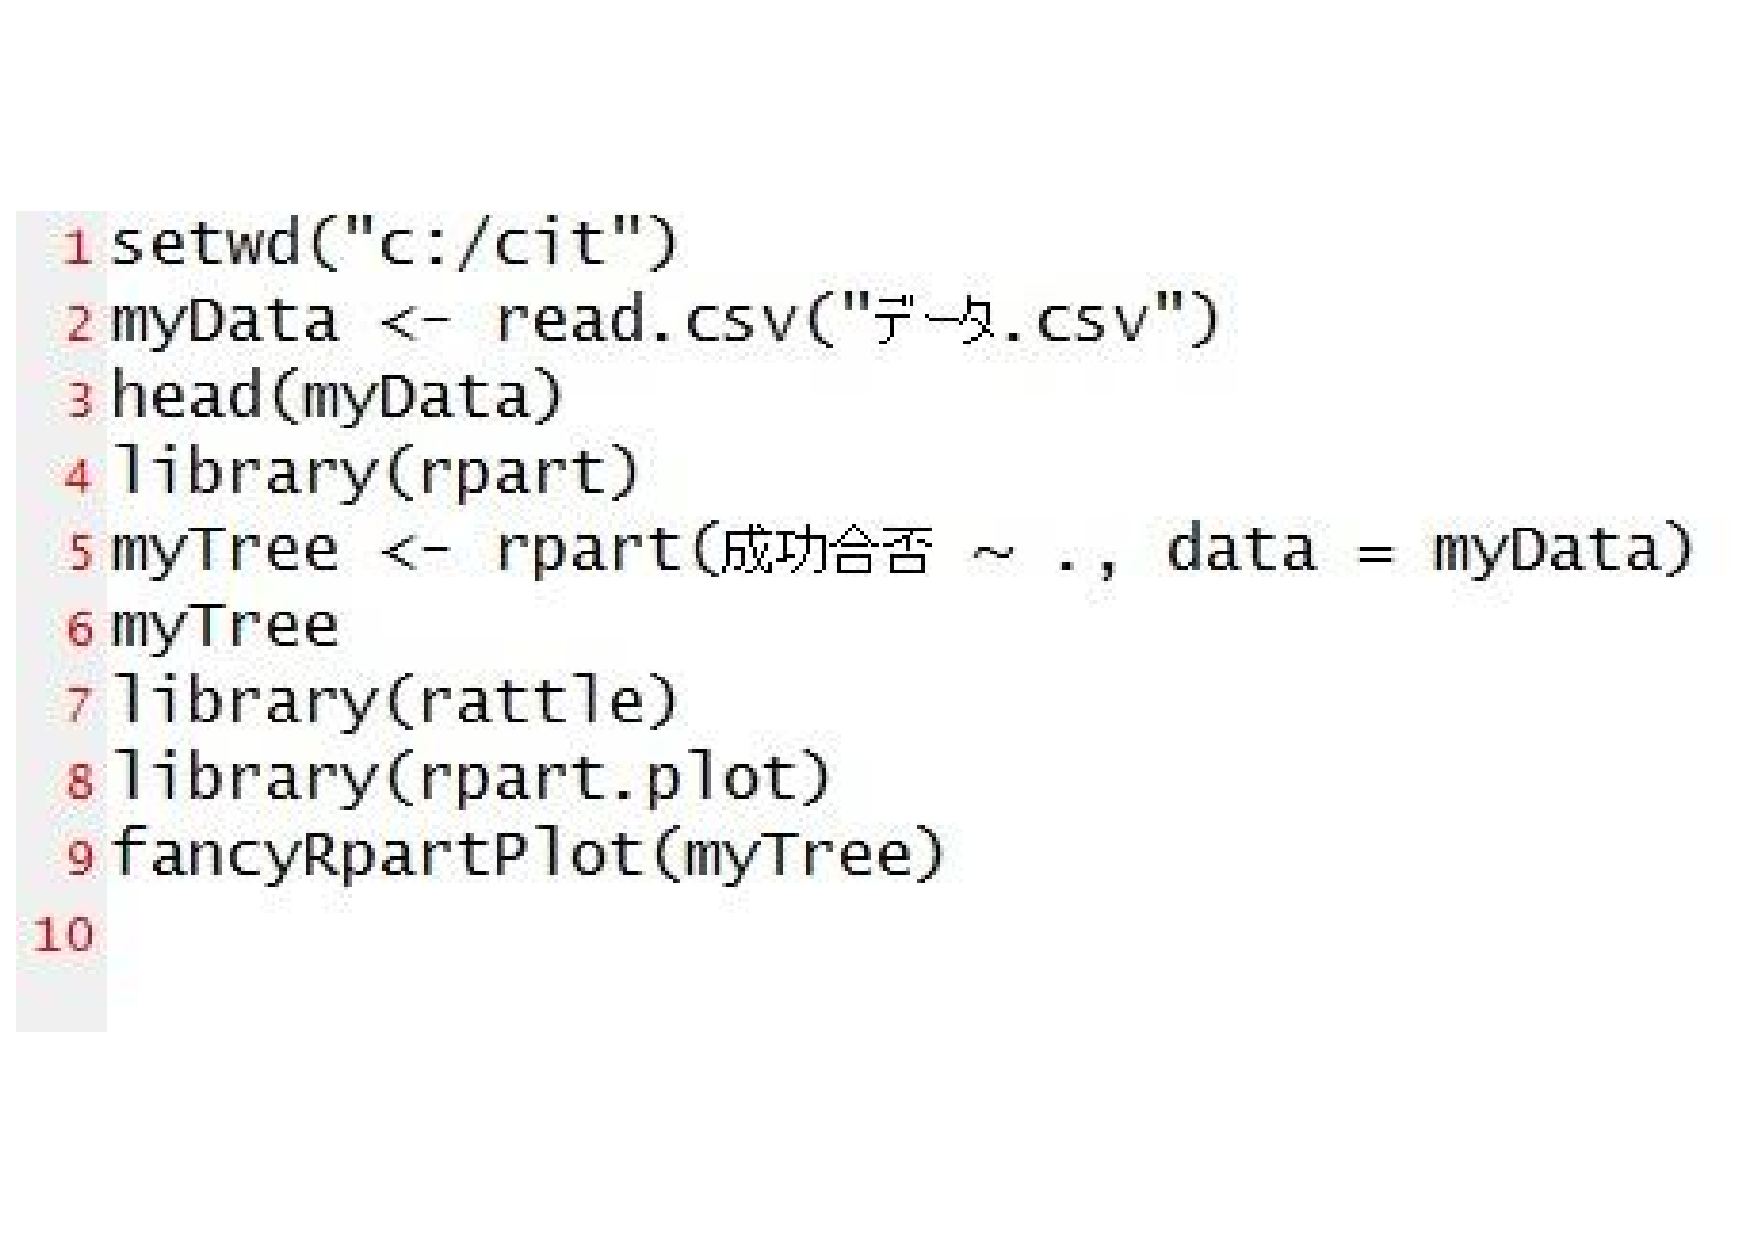
\includegraphics[width=13cm]{figure21.pdf}
\caption{決定木を書くコマンド}\label{sannp}
\end{figure}

コマンドを実行すると以下のように決定木を得ることができる.
\begin{figure}[H]
\centering
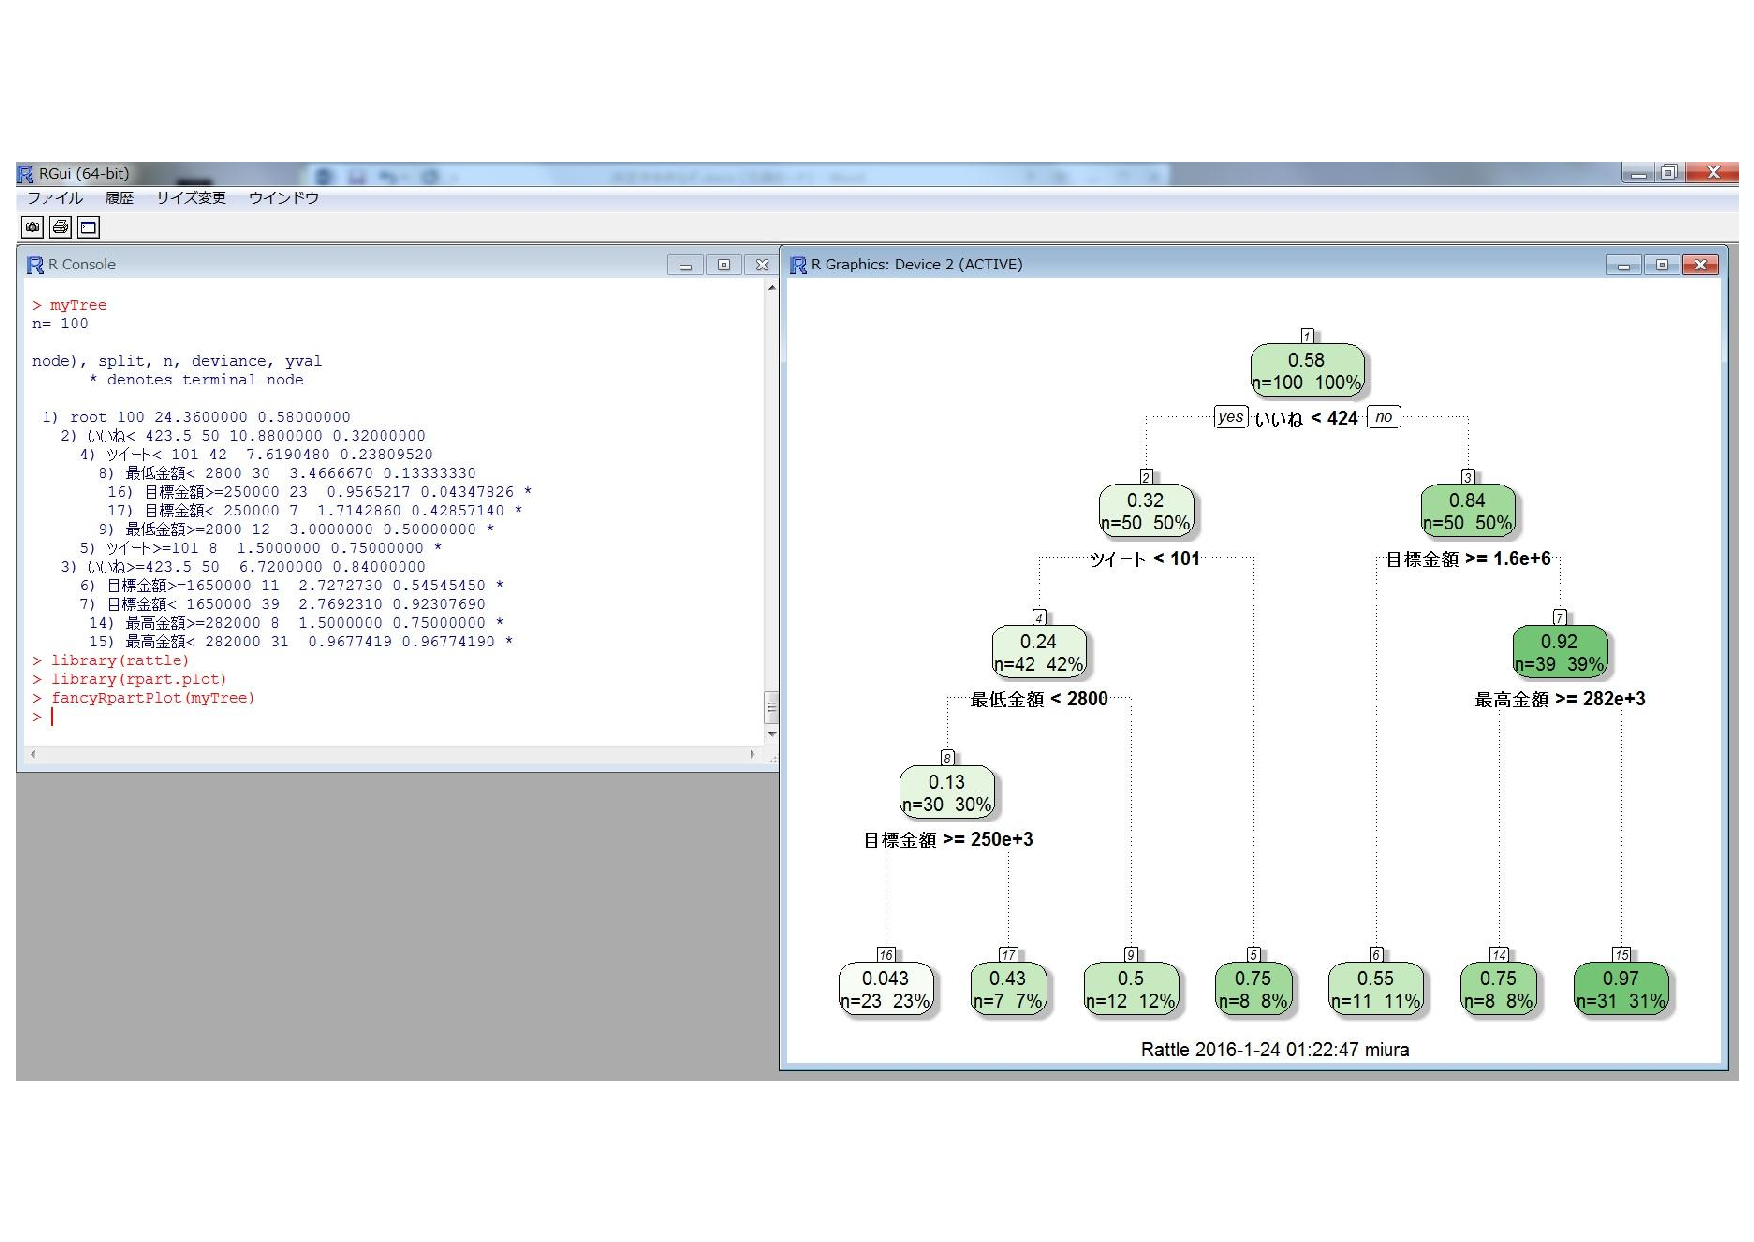
\includegraphics[width=13cm]{figure22.pdf}
\caption{コマンドの結果}\label{sannp}
\end{figure}

\section{ブートストラップ法について}
決定木分析はデータによって得られる決定木が大きく変わってしまうため,信用度が低い言われることがある.
そのため今回は,決定木分析を行う際に組み合わせを変えた場合の成否の一致率から決定木の精度を出すこととする.
その際にブートストラップ法を用いて数パターンの決定木を書くこととする.

ブートストラップ法とは使用するデータの組み合わせから擬似的にサンプルの数を増やす手法であり,信頼区間や結果の修整などを推測する場合に使われる.また集めることが困難なデータを使用する場合などにも使用されている.実際にブートストラップを行ったものを下記に記載する.
\begin{figure}[H]
\centering
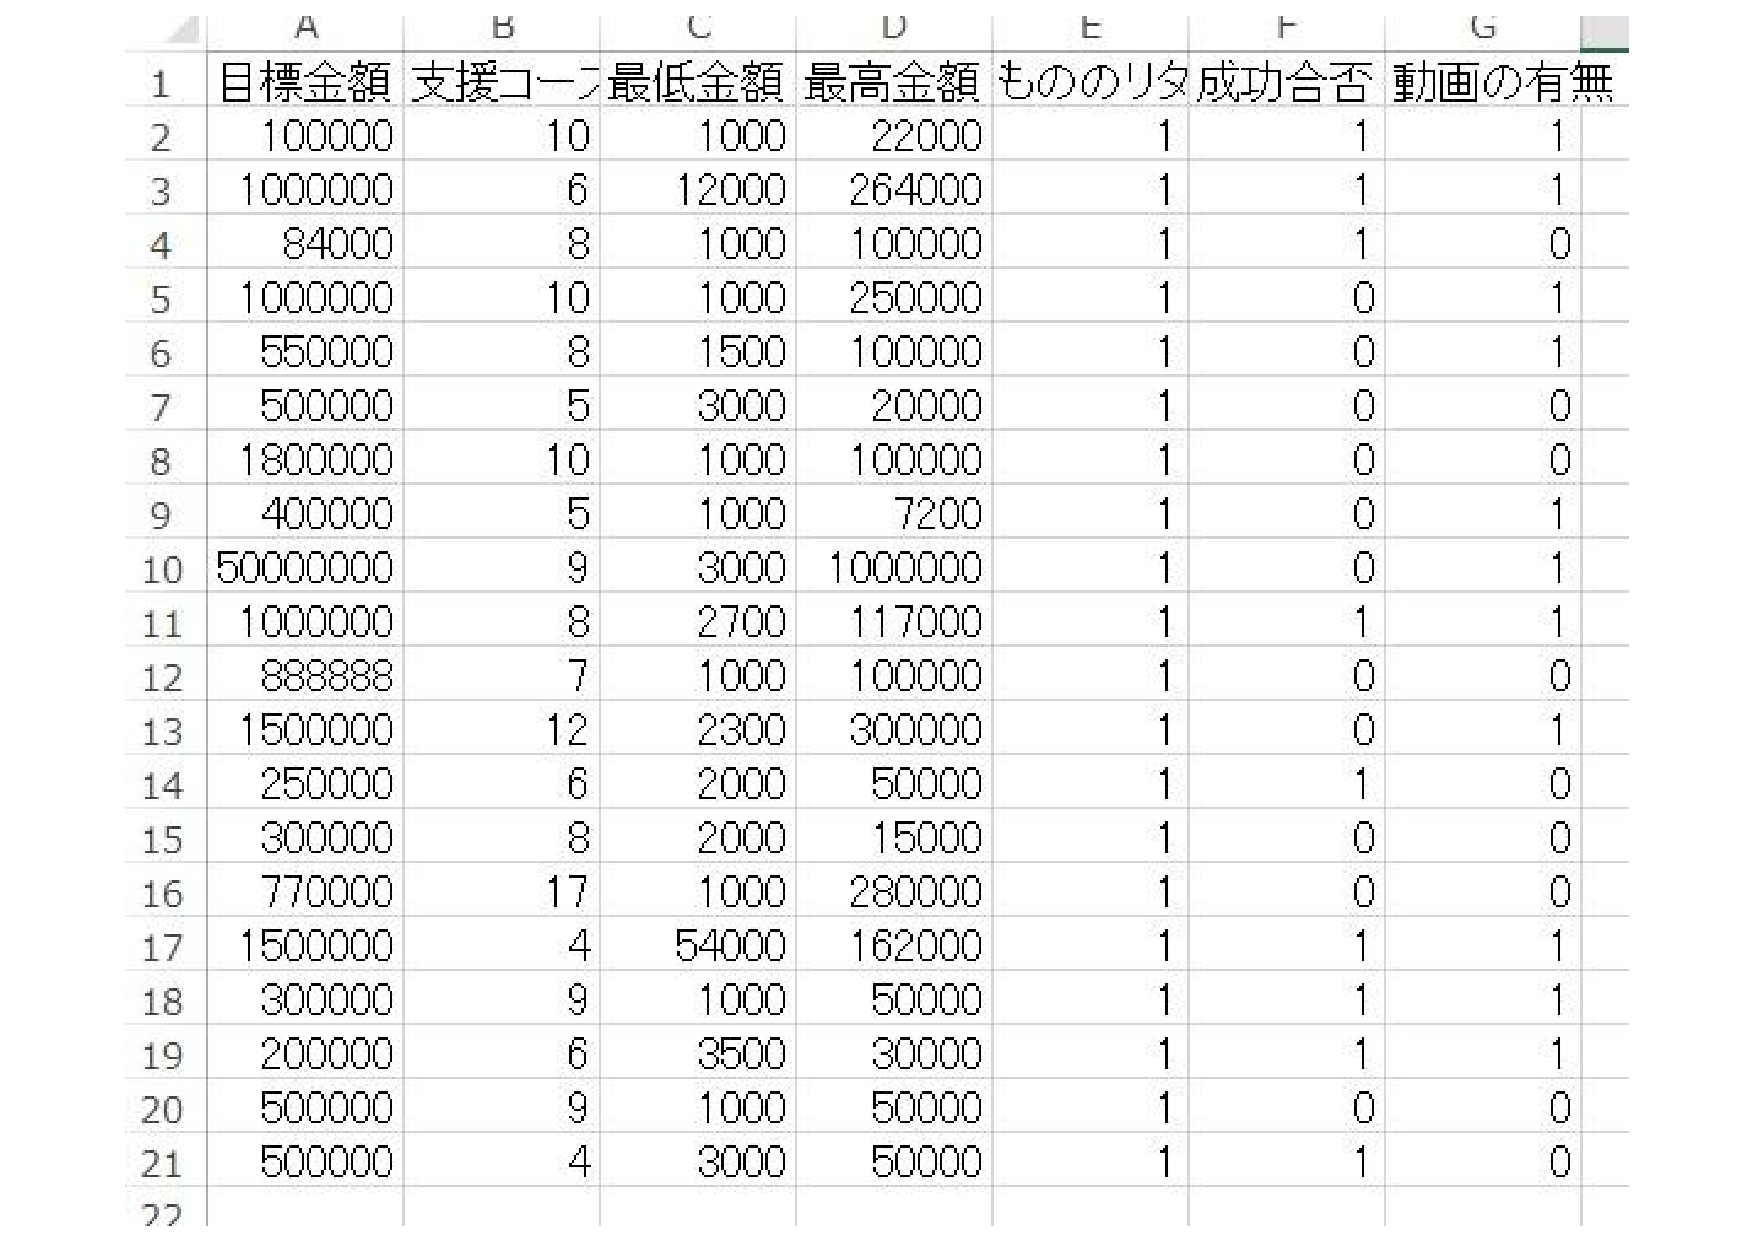
\includegraphics[width=13cm]{figure41.pdf}
\caption{ブートストラップ1のデータ}\label{sannp}
\end{figure}

\begin{figure}[H]
\centering
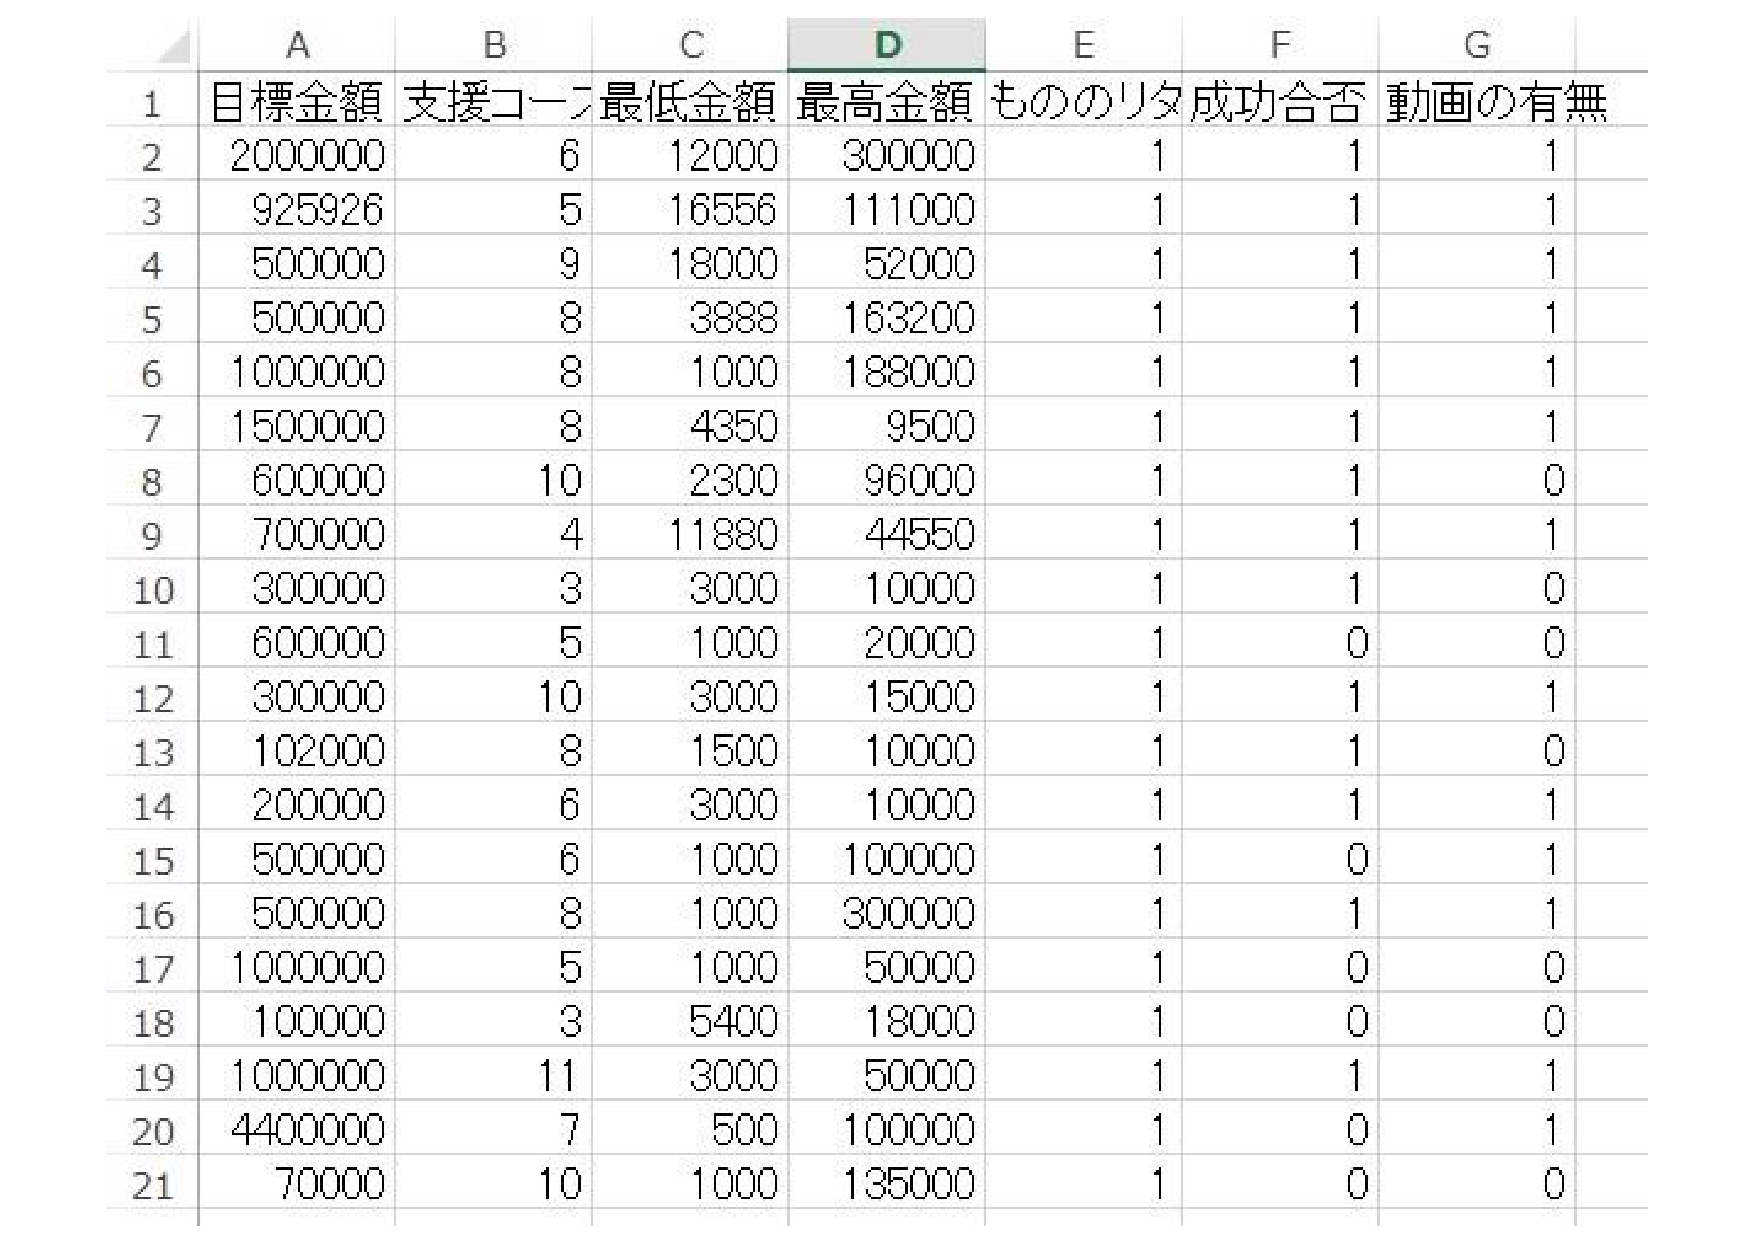
\includegraphics[width=13cm]{figure42.pdf}
\caption{ブートストラップ2のデータ}\label{sannp}
\end{figure}

\begin{figure}[H]
\centering
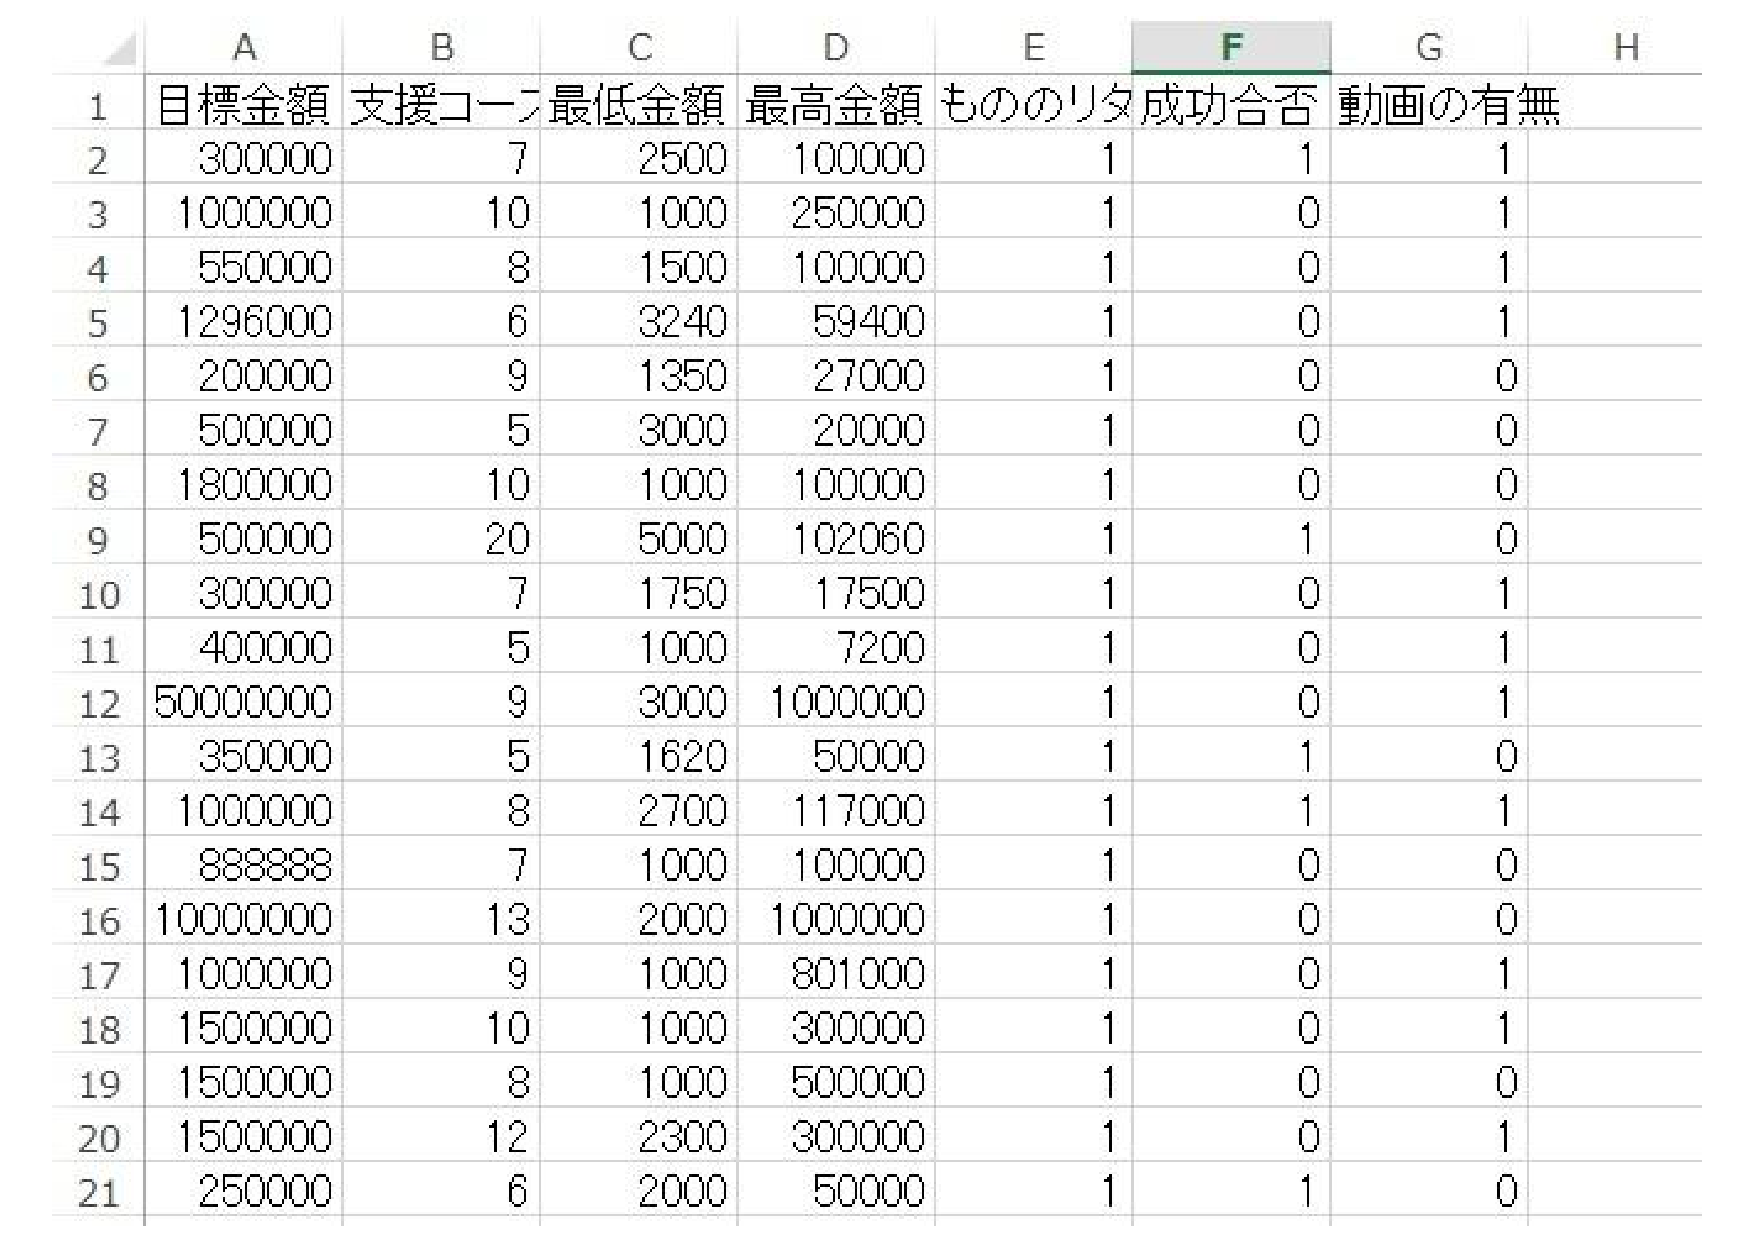
\includegraphics[width=13cm]{figure43.pdf}
\caption{ブートストラップ3のデータ}\label{sannp}
\end{figure}

\begin{figure}[H]
\centering
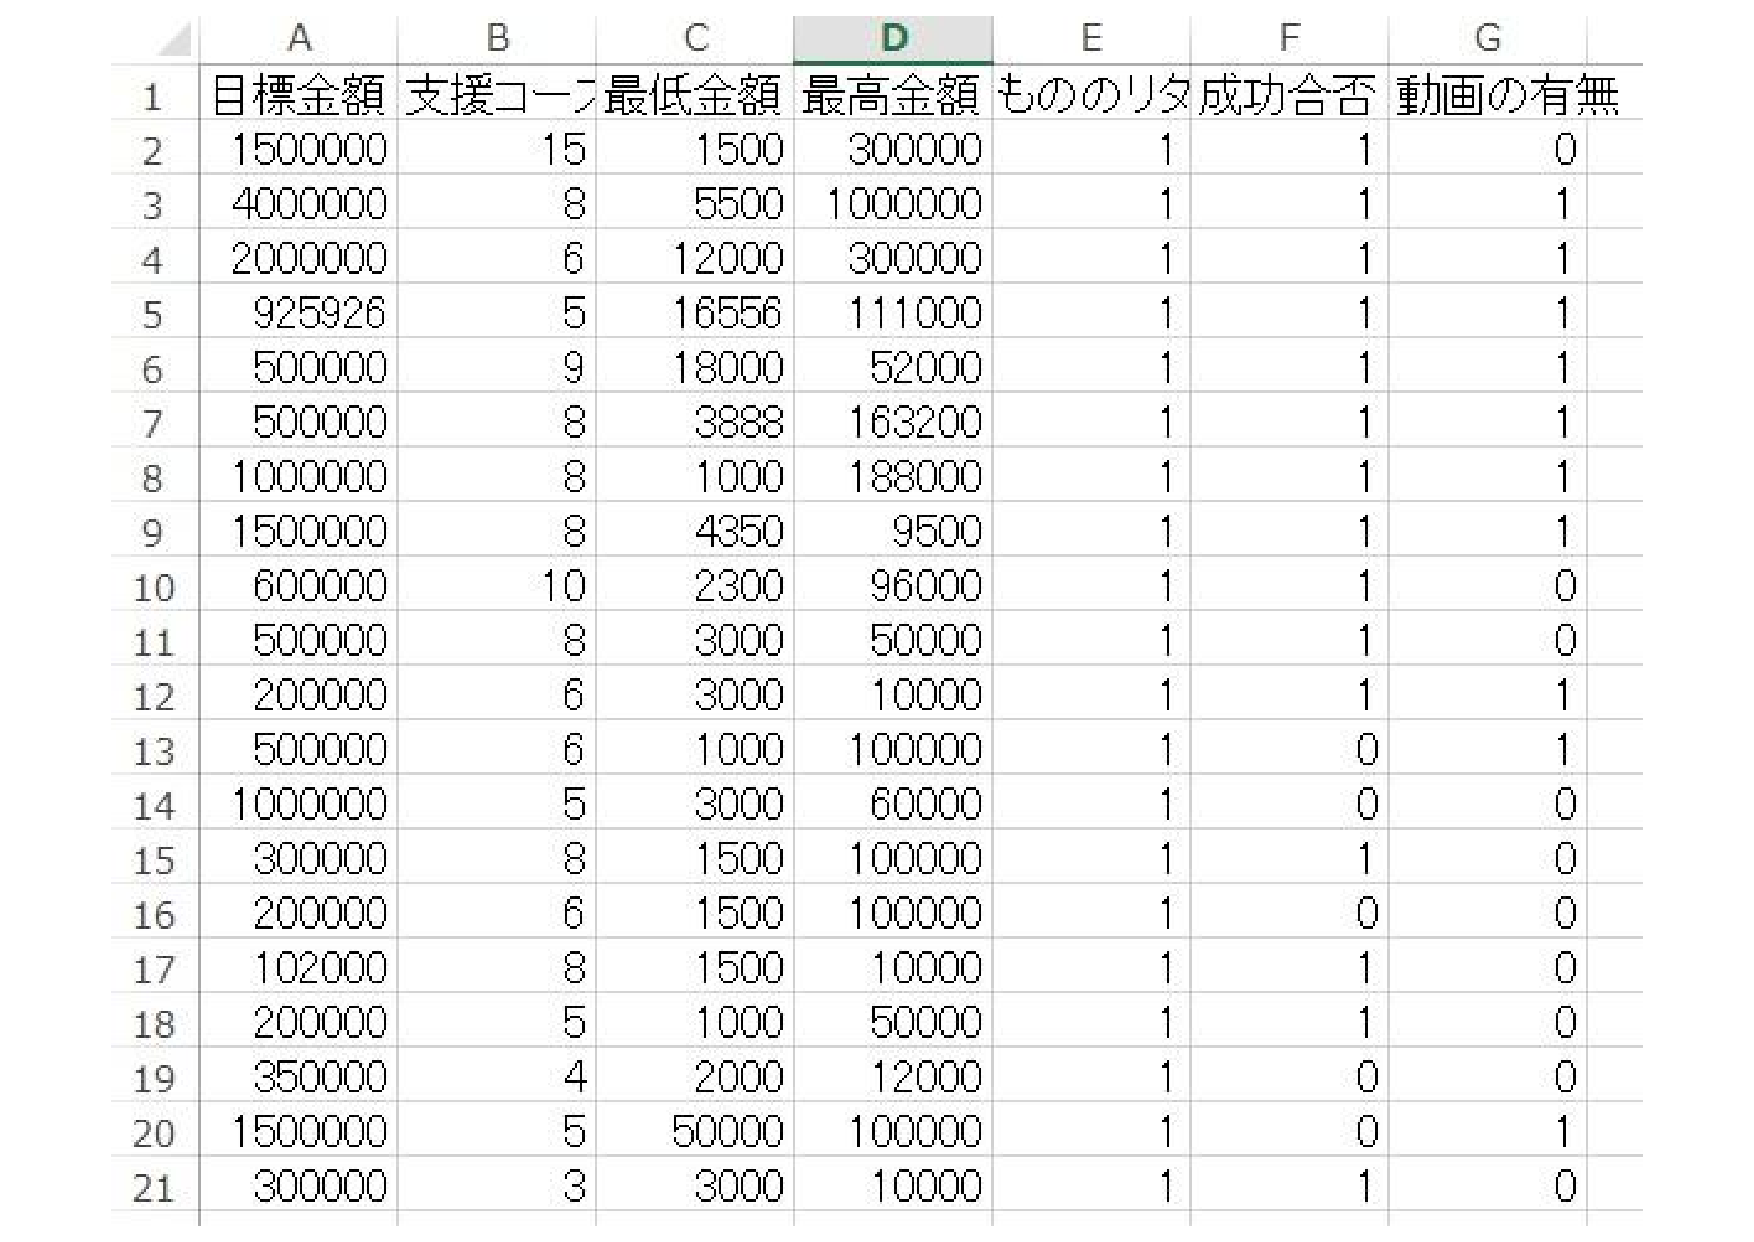
\includegraphics[width=13cm]{figure50.pdf}
\caption{ブートストラップ4のデータ}\label{sannp}
\end{figure}

\begin{figure}[H]
\centering
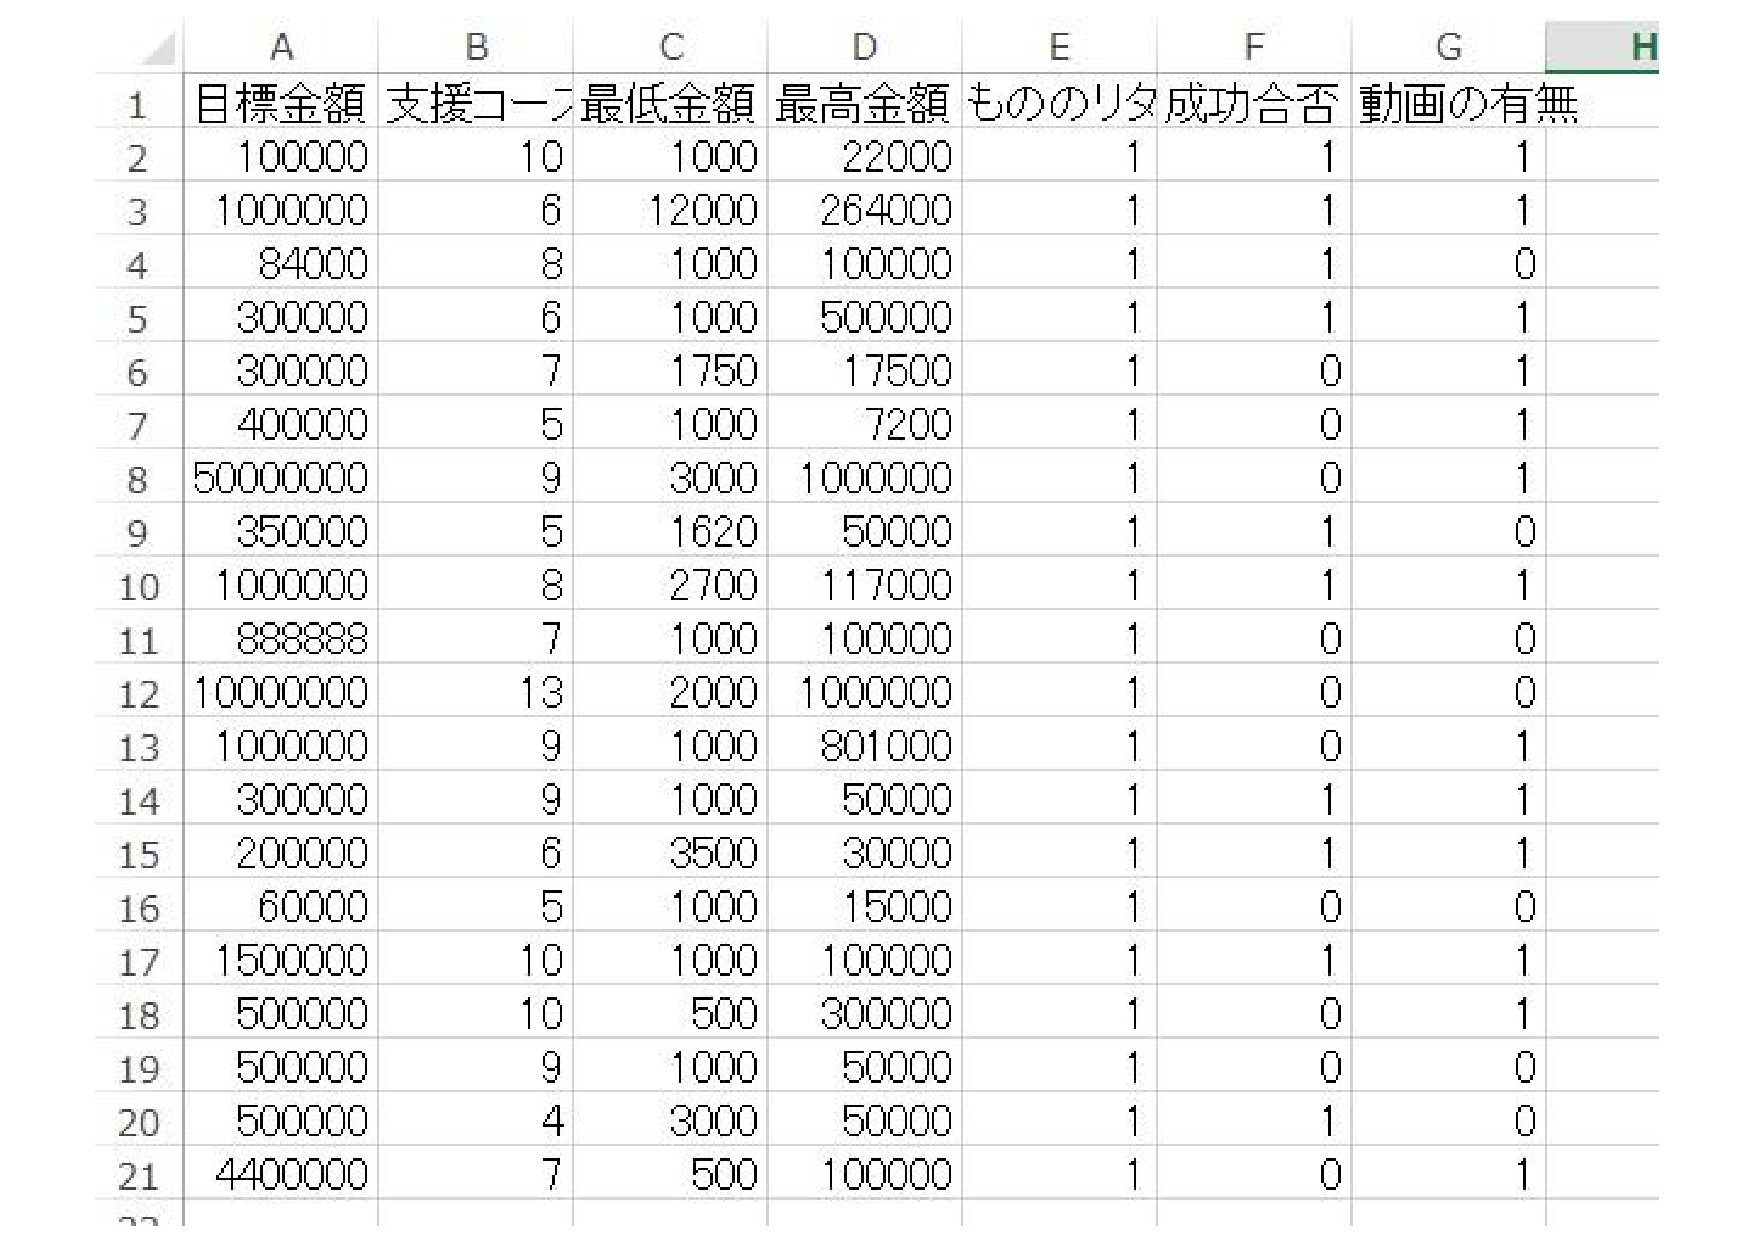
\includegraphics[width=13cm]{figure51.pdf}
\caption{ブートストラップ5のデータ}\label{sannp}
\end{figure}

\begin{figure}[H]
\centering
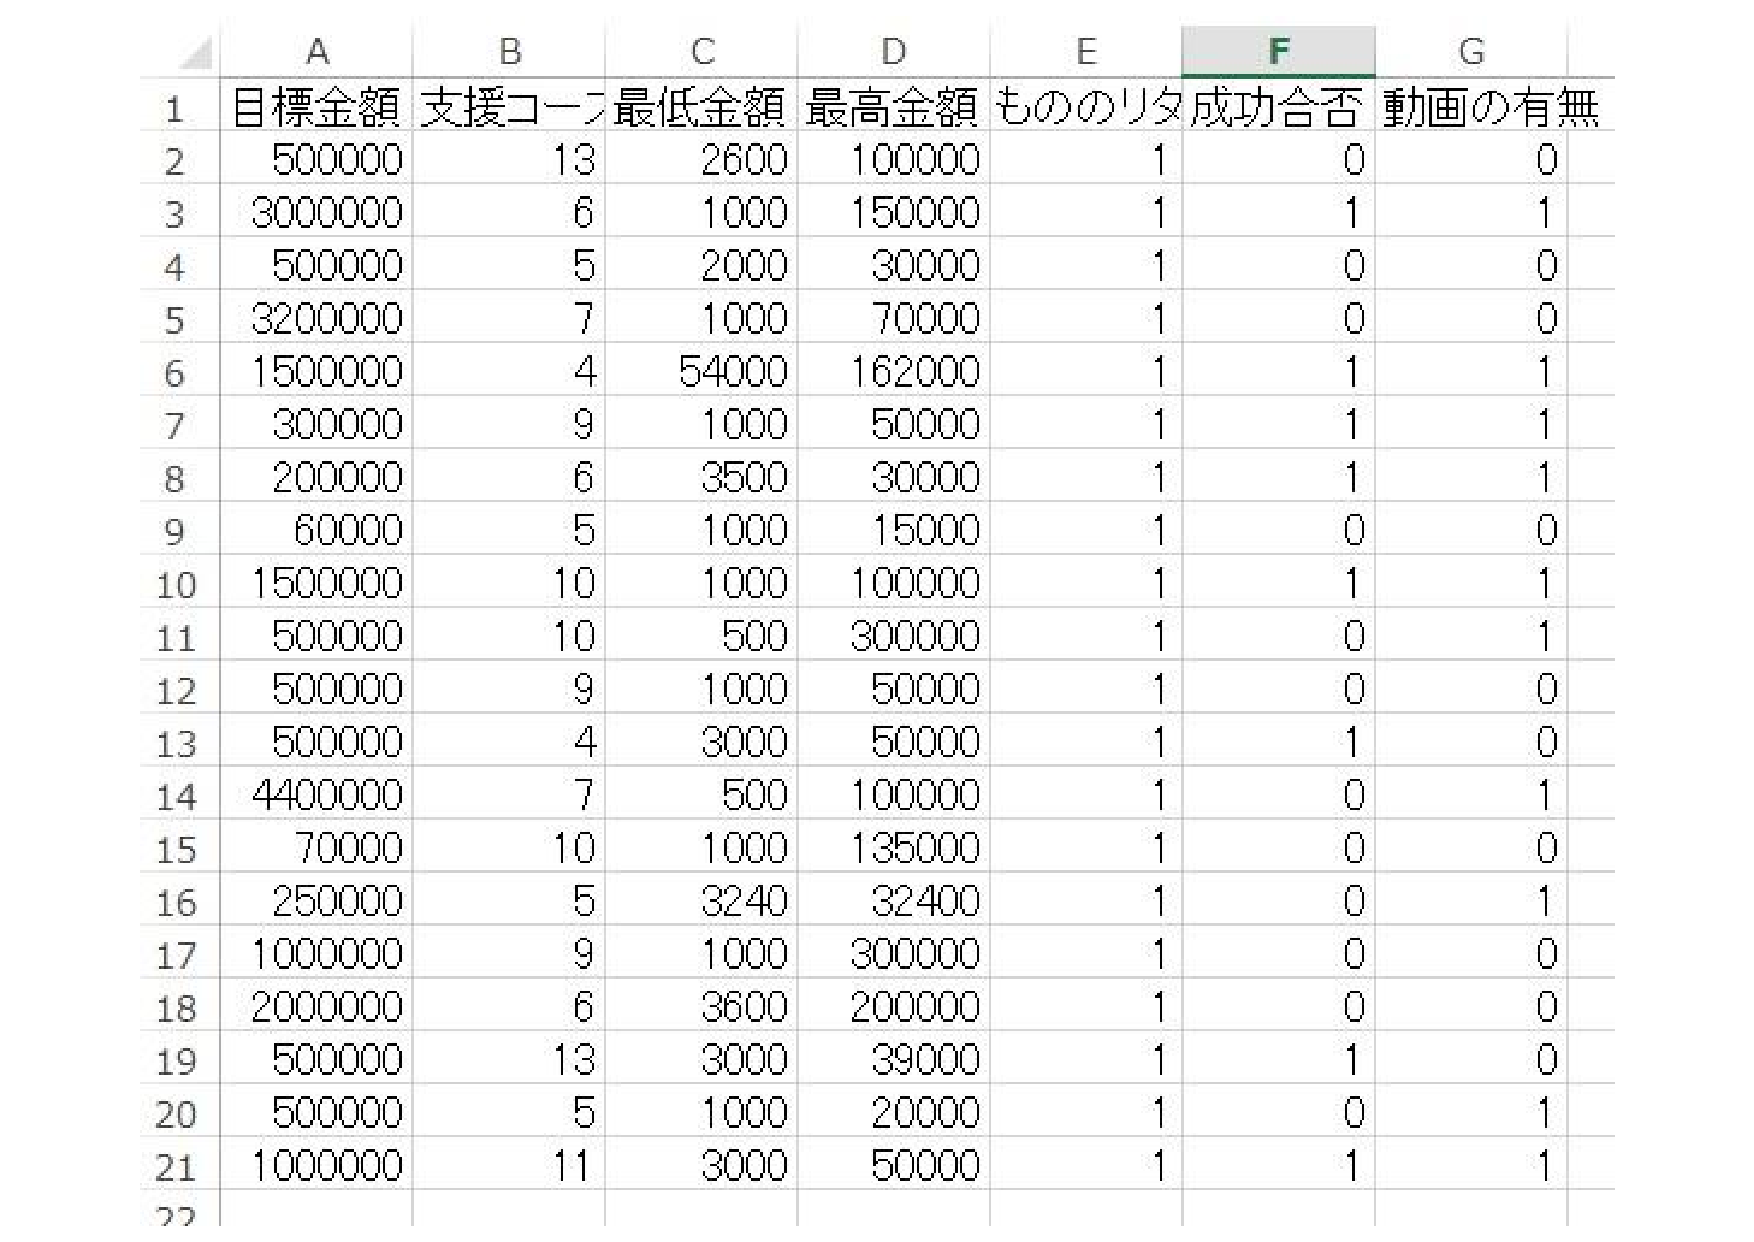
\includegraphics[width=13cm]{figure53.pdf}
\caption{ブートストラップ6のデータ}\label{sannp}
\end{figure}

\begin{figure}[H]
\centering
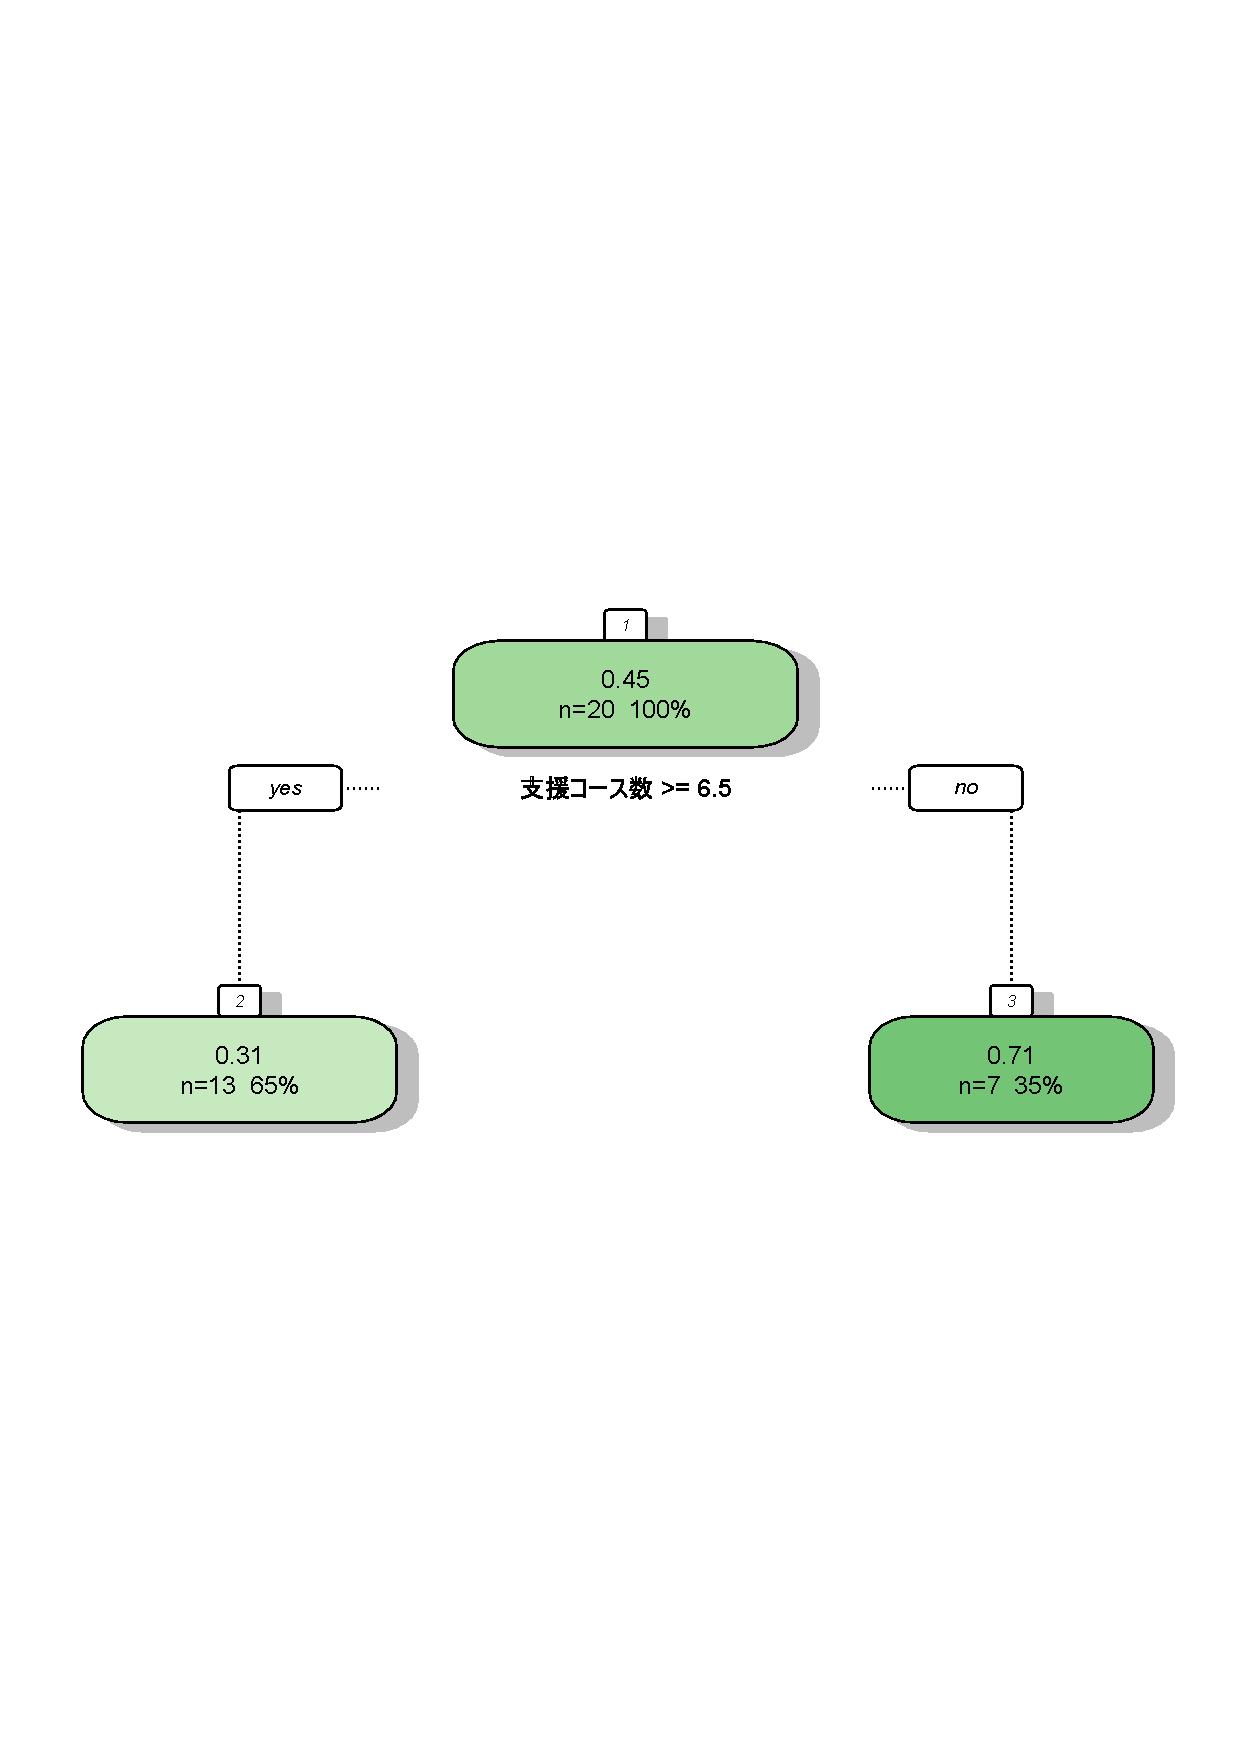
\includegraphics[width=13cm]{figure38.pdf}
\caption{ブートストラップ1}\label{sannp}
\end{figure}

\begin{figure}[H]
\centering
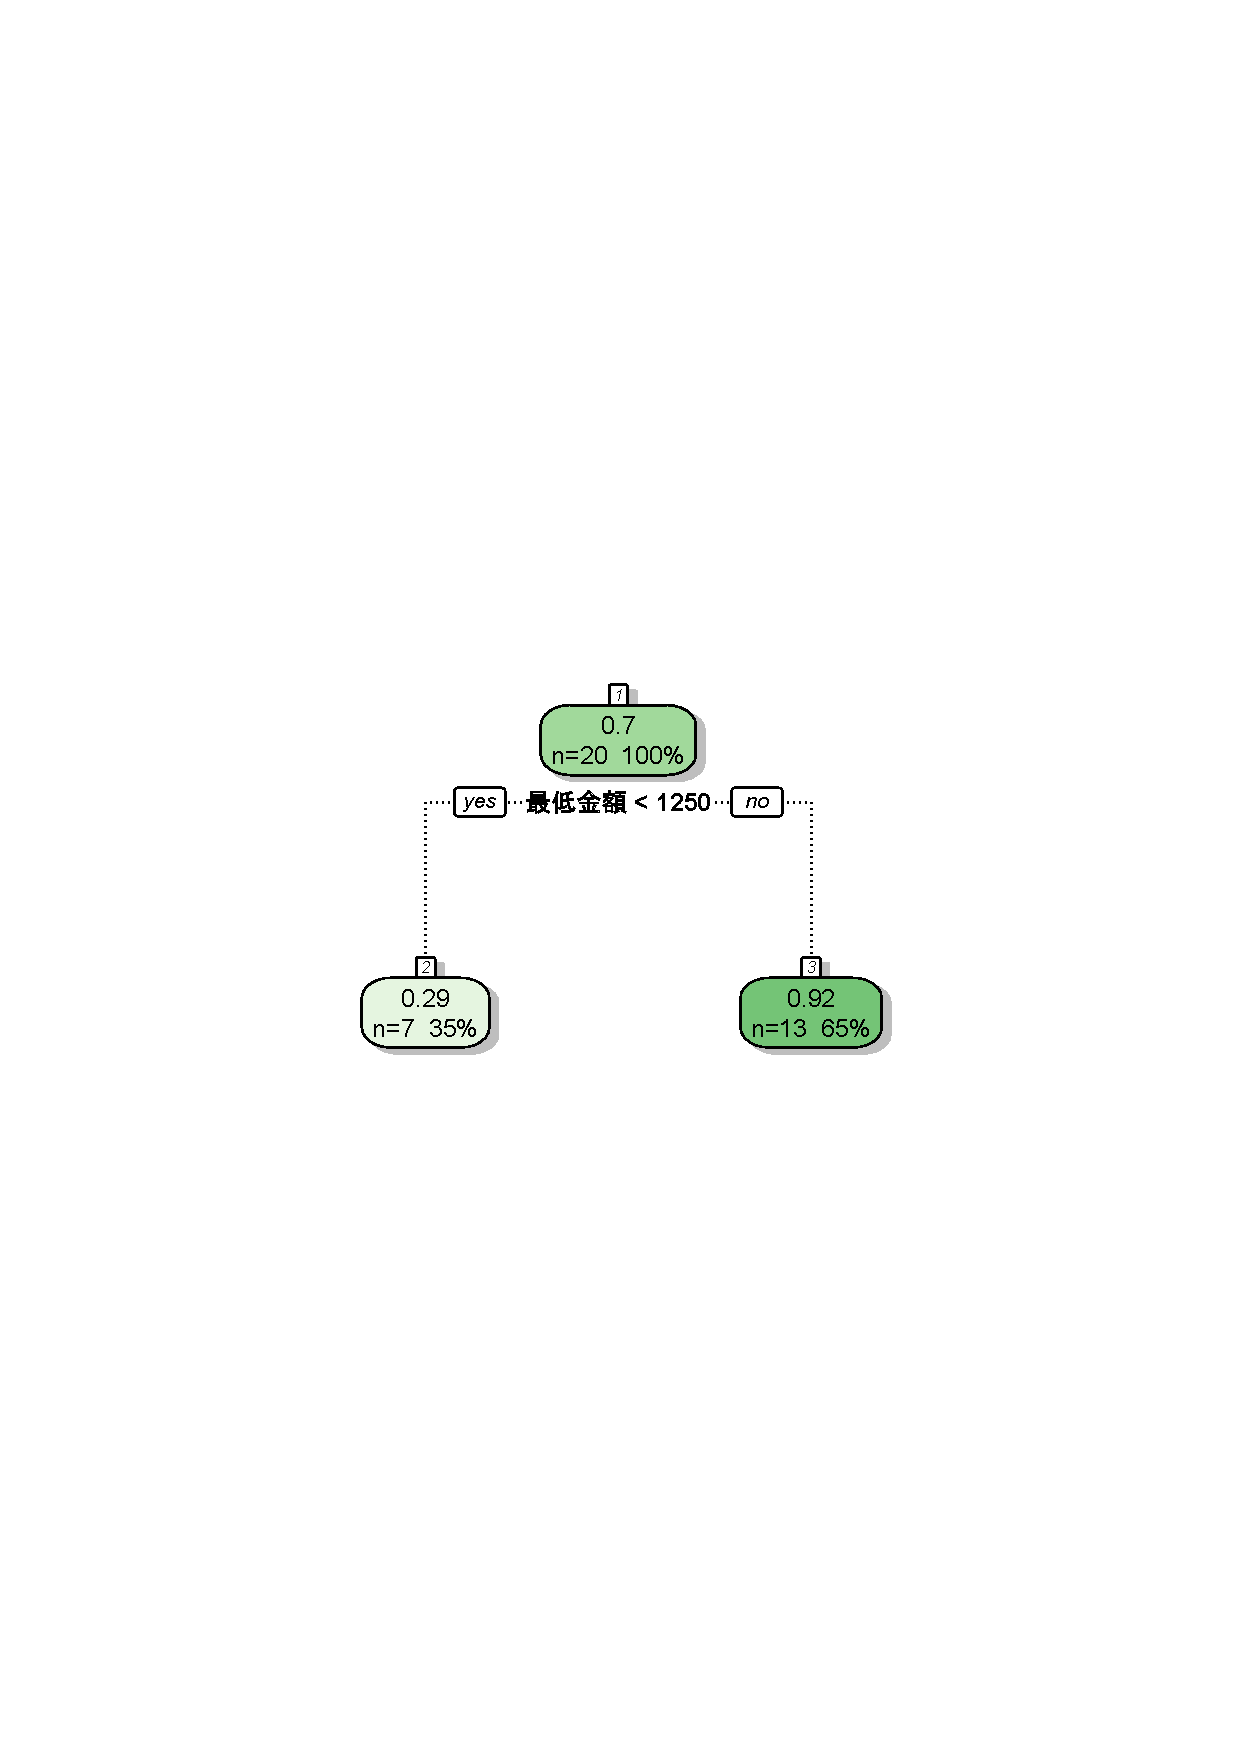
\includegraphics[width=13cm]{figure39.pdf}
\caption{ブートストラップ2}\label{sannp}
\end{figure}

\begin{figure}[H]
\centering
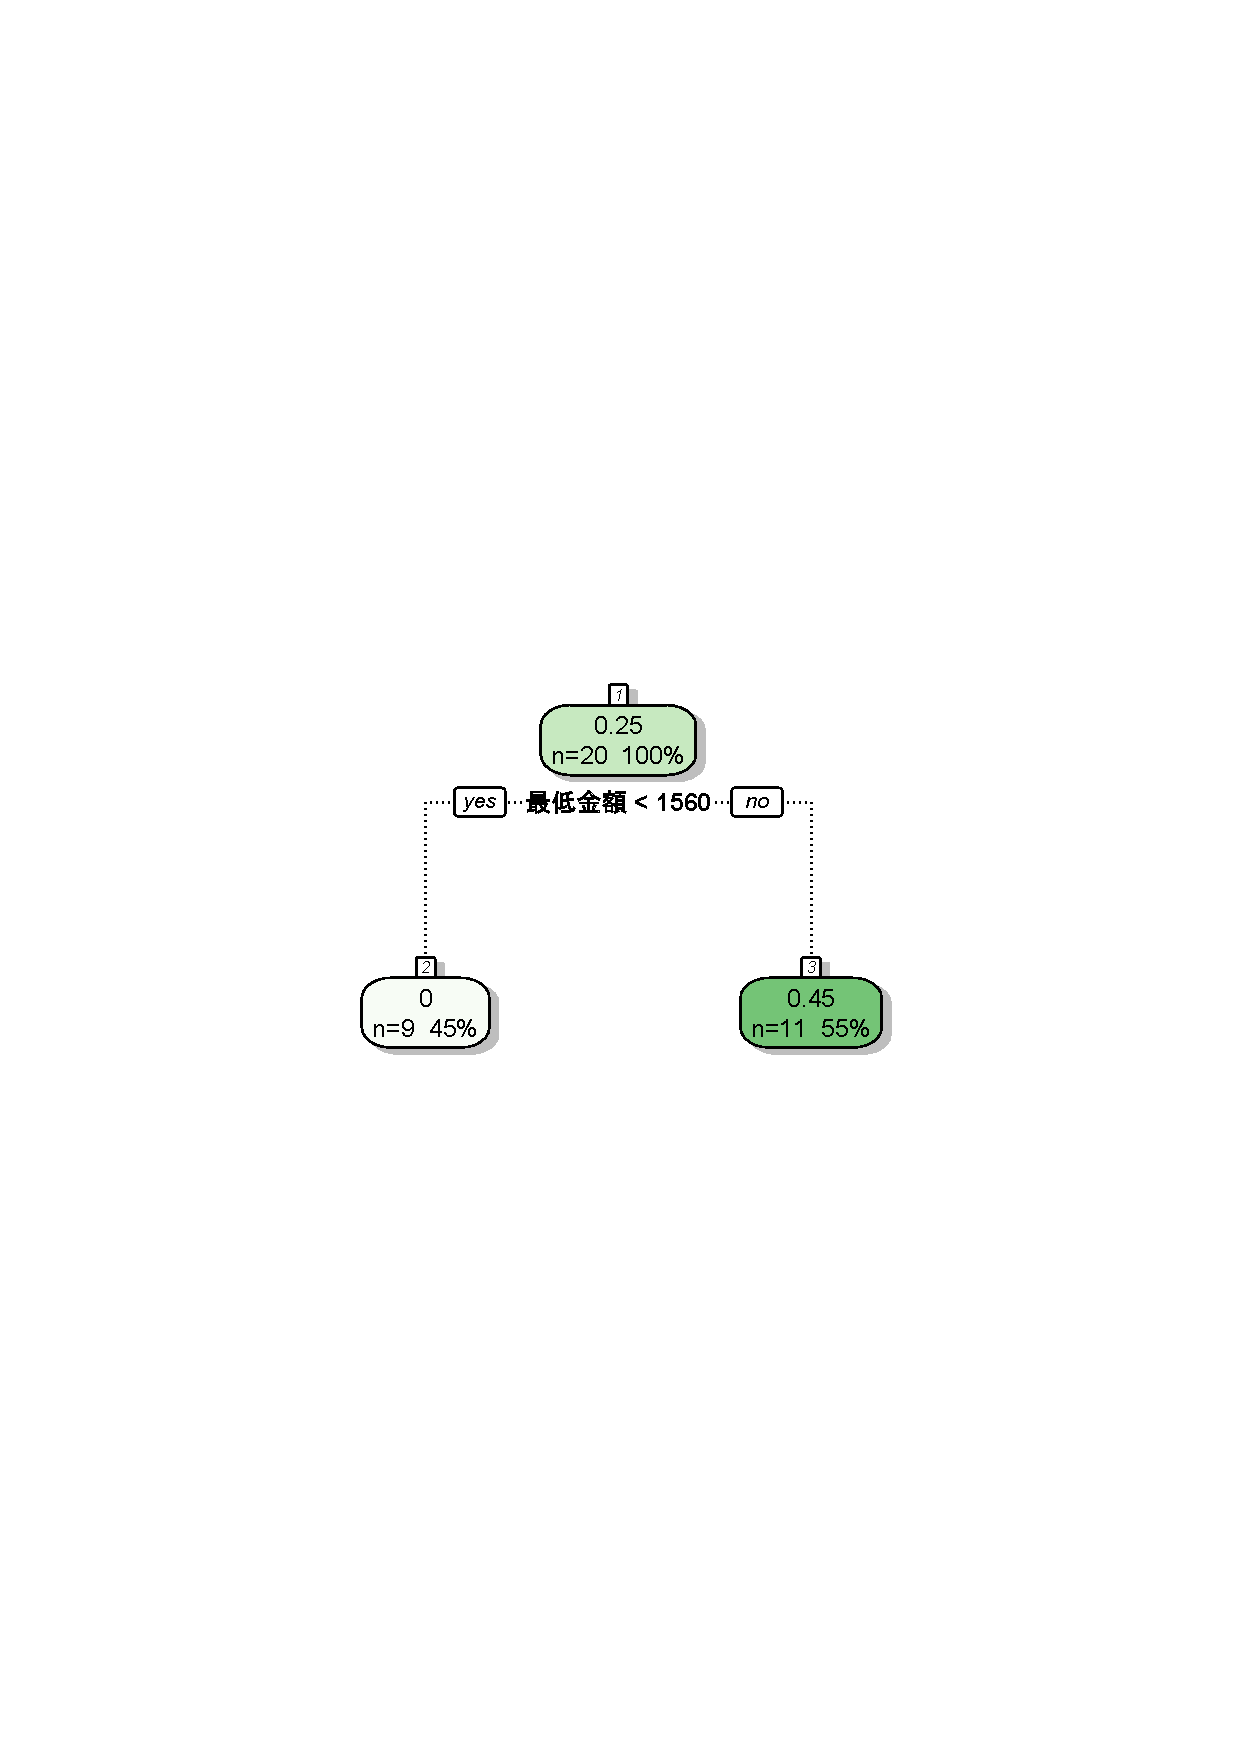
\includegraphics[width=13cm]{figure40.pdf}
\caption{ブートストラップ3}\label{sannp}
\end{figure}

\begin{figure}[H]
\centering
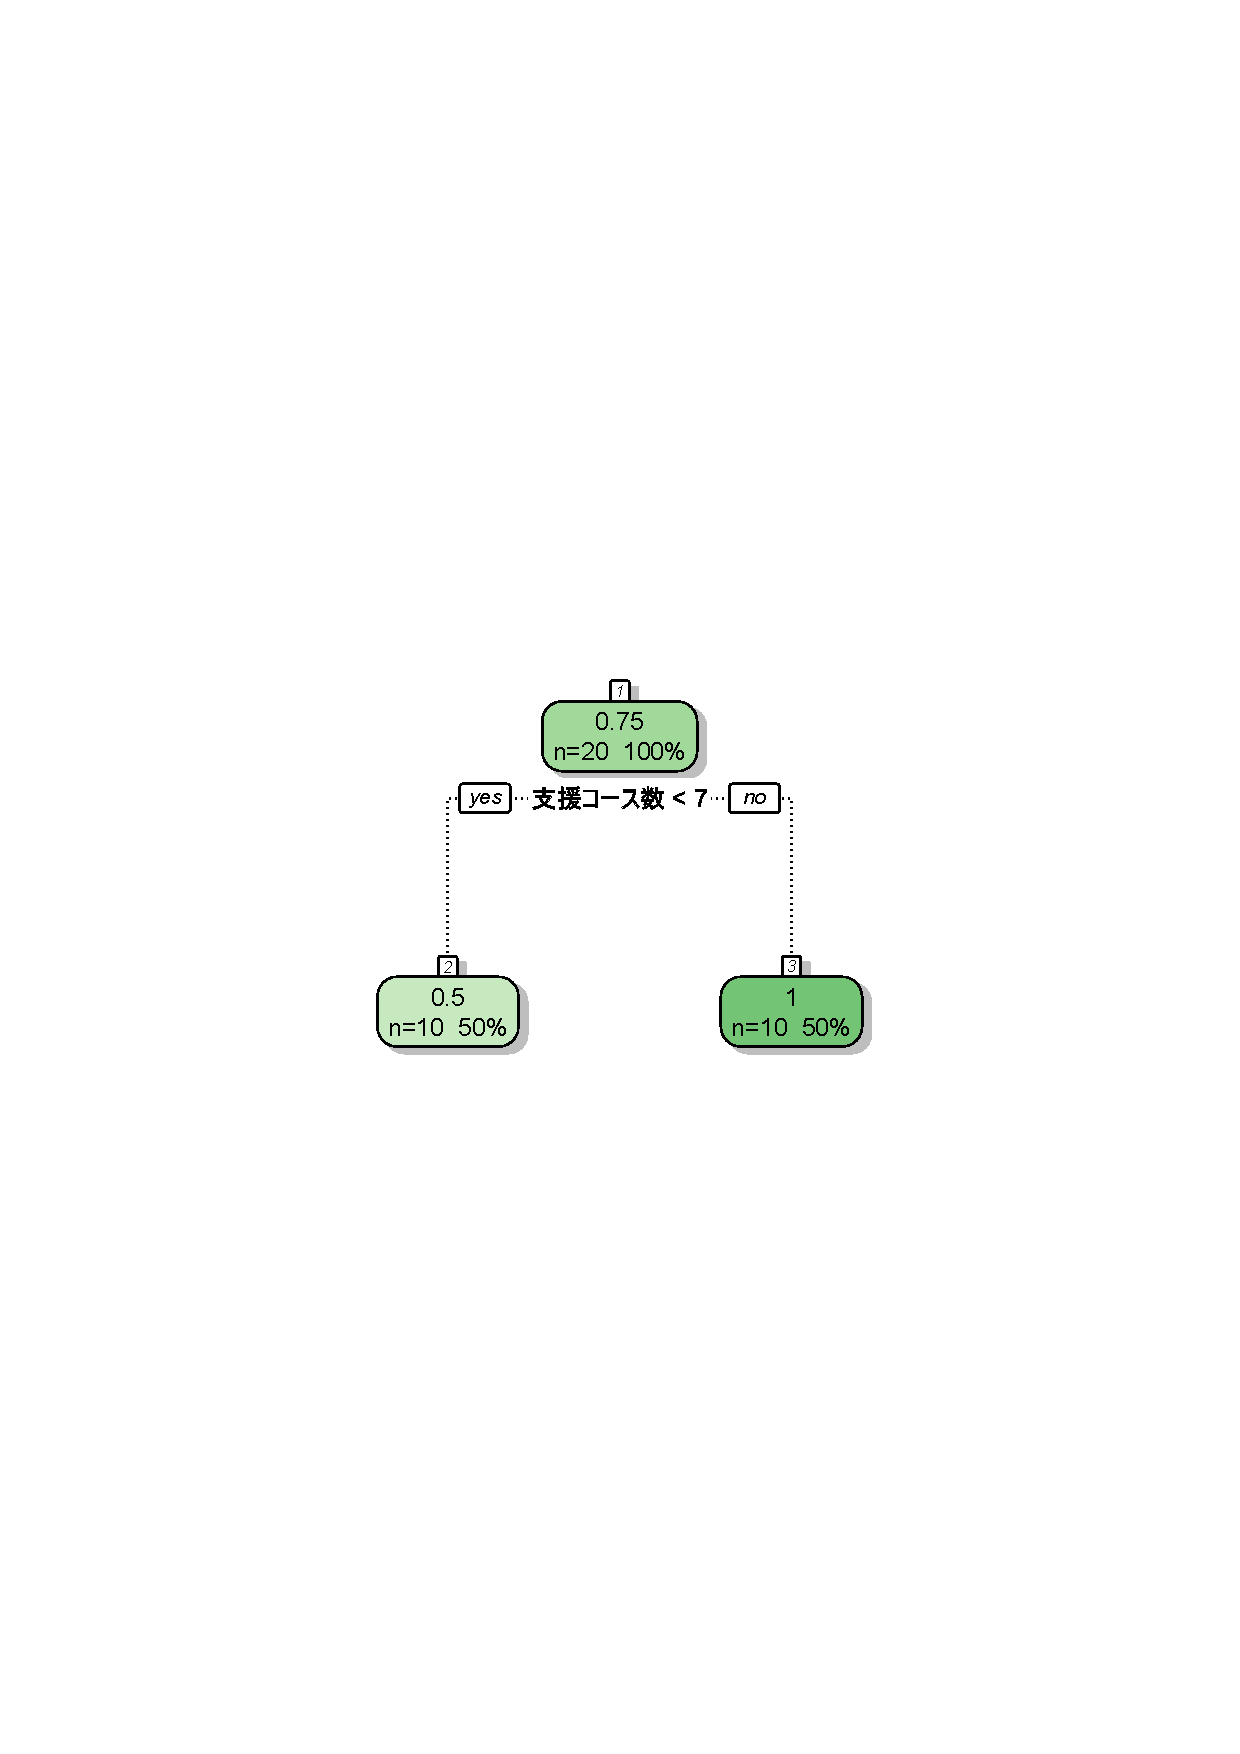
\includegraphics[width=13cm]{figure48.pdf}
\caption{ブートストラップ4}\label{sannp}
\end{figure}

\begin{figure}[H]
\centering
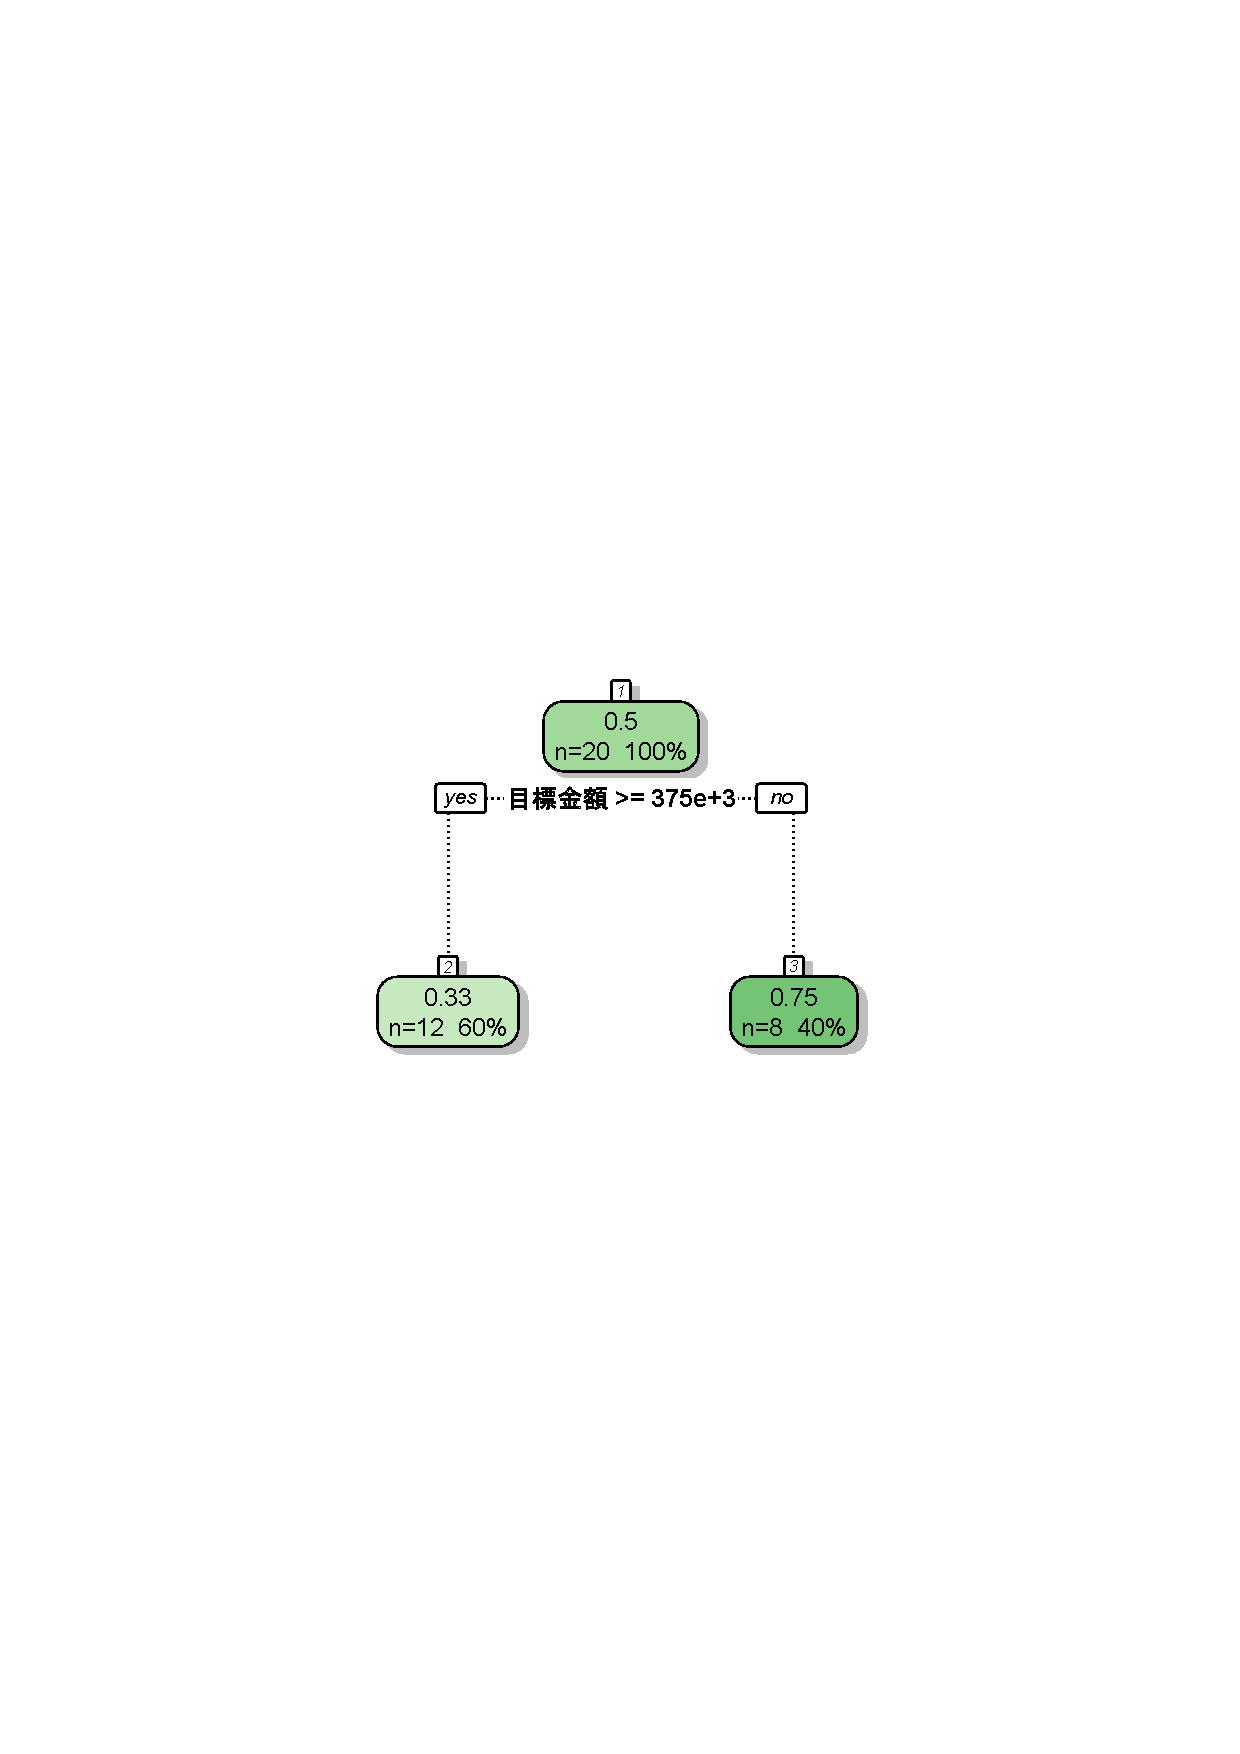
\includegraphics[width=13cm]{figure49.pdf}
\caption{ブートストラップ5}\label{sannp}
\end{figure}

\begin{figure}[H]
\centering
\includegraphics[width=13cm]{figure52.pdf}
\caption{ブートストラップ6}\label{sannp}
\end{figure}

このようにサンプルの種類を変えることで別の結果を得ることができる.使用した要因は全件で行う決定木分析と同じ,目標金額・支援コース数・支援最低金額・支援最高金額・リターンの有無・動画の有無を使用した.

6回のブートストラップとも分岐は1つであり,分岐の要因は支援コース数が2回,支援最低金額が3回,目標金額が1回となった.回数が少ないため信憑性にかけるものの支援最低金額が3回出現していることから成功に強く関わる要因であることが考えられる.


\chapter{結果・考察}
決定木分析で得られた決定木が以下である.実際との一致率は83\%であった.


\begin{figure}[H]
\centering
\includegraphics[width=13cm]{figure19.pdf}
\caption{得られた決定木1}\label{sannp}
\end{figure}

得られた決定木から,支援最低金額が3,744 円から35,990 円で目標金額が375,000 円以上のプロジェクトの成功率が最も高くなることがわかる.これは支援最低金額でリターンがもらえるプロジェクトが成功しやすいためだと思われる.

支援最低金額が500 円や1,000 円のコースは,お礼のメールや手紙が届くものが多いが,支援最低金額が3,000 円や5,000 円程度の額であるとCDや出版物がもらえるようになり,それを目当てにした支援者が多いということもあるだろう.目標金額が375,000 円以上の場合の成功率が高くなることは,この目標金額が今回調査したプロジェクトの平均目標金額(160,6724 円)よりかなり低く,そのことが資金調達のしやすさに影響しているためだと思われる.

また最低金額と目標金額が決定木に頻出することからも,この2つの設定額が重要であることがわかる.

次に,100件のプロジェクトの70件で組み合わせを変えて5回決定木を書き,残りの30件で実際の成否との一致率を調べた.


\begin{figure}[H]
\centering
\includegraphics[width=13cm]{figure24.pdf}
\caption{得られた決定木2}\label{sannp}
\end{figure}


決定木2は28件が一致していた.一致率は92.4\%である.この決定木の一致率が著しく高く,テストデータと学習データがかみ合っていた可能性が考えられる.

\begin{figure}[H]
\centering
\includegraphics[width=13cm]{figure25.pdf}
\caption{得られた決定木3}\label{sannp}
\end{figure}


決定木3は15件が一致していた.一致率は49.5\%である.一致率は5回中一番低いものの一番短く綺麗なな決定木を書くことができた.
テストデータのほうに大多数のプロジェクトとは別の動きをしたものが多くあった可能性が考えられる.

\begin{figure}[H]
\centering
\includegraphics[width=13cm]{figure26.pdf}
\caption{得られた決定木4}\label{sannp}
\end{figure}

決定木4は20件が一致していた.一致率は66\%である

\begin{figure}[H]
\centering
\includegraphics[width=13cm]{figure27.pdf}
\caption{得られた決定木5}\label{sannp}
\end{figure}

決定木5は22件が一致していた.一致率は72.6\%である

\begin{figure}[H]
\centering
\includegraphics[width=13cm]{figure28.pdf}
\caption{得られた決定木6}\label{sannp}
\end{figure}

決定6は19件が一致していた.一致率は62.7\%である


5つの決定木の実際の成否との一致率の平均が68.64\%であり,テストデータと学習データを分けて決定木を書いても十分な一致率を求めることができた.

決定木毎に一致率のばらつきが大きく,決定木の特性である安定性にかける部分を補うには何本も決定木を描くことで平均を取ることがよいと考えられる.

また支援最低金額がどの決定木においても上位に来ることから,特に重要なことが伺え,全件で決定木を書いたときと同じ結果が得られた.

全件で重要だと考えられていた,目標金額の位置は頻度的に多いが支援コース数と同じ程度であり,支援コース数と目標金額の重要度は同じくらいだと考えられる.

分析に用いる要因に,そのプロジェクトに対して付けられたFacebook の「いいね」の数と,そのプロジェクトのURL がTwitter でつぶやかれた回数を加えた場合の決定木が下記である.

\begin{figure}[H]
\centering
\includegraphics[width=13cm]{figure23.pdf}
\caption{得られた決定木7}\label{sannp}
\end{figure}

Facebook の「いいね」ボタンやTwitter の「ツイート」ボタンを利用された数が大きいプロジェクトは成功している傾向にあり,SNS で広報を積極的に行うことが成功に繋がると考えられる.決定木の上に位置する要因ほど重要度が高くなることからもこれが言えるであろう.

この2つの要因は自分で意図的に操作することは難しいがSNS を通してプロジェクトの進捗状況を報告したり,SNS での反応に対して対応をすることで数を増やすことは多少可能であり,操作までとは言えないものの伸ばす努力は十分に可能であると考えられる.


\section{結論}
クラウドファンディングにおいて,プロジェクトの内容以外の成功要因を,決定木分析によって調査した.

決定木の予測が実際の結果とよく合っていることから,そのような要因が存在することが示唆される.

今回結果から以下のことが言えると考える.
\begin{itemize}
\item 支援最低金が今回使った要因の中でもっとも重要である.
 \item SNSを利用した広報活動が非常に有効である.
 \item 今回作成した決定木は実用に耐えるものである.
\end{itemize}

決定木の数を増やすことやプロジェクト数を増やすことで信憑性をあげるとともに,数値の推移で成否を判別してみるような別のアプローチを取るとさらに結果が出ると考える.

また成功要因と考えられるものを増やし,ロジスティック分析を使い,関わりが少ない要因をそぎ落とし精度の高い分析を行うことなど,研究を行ったことで課題が出てきた.


\bibliographystyle{junsrt}
\bibliography{biblio}%「biblio.bib」というファイルが必要.



\end{document}
